
% ---------- Titelblad Masterproef Faculteit Wetenschappen -----------
% Dit document is opgesteld voor compilatie met pdflatex.  Indien je
% wilt compileren met latex naar dvi/ps, dien je de figuren naar
% (e)ps-formaat om te zetten.
%                           -- december 2012
% -------------------------------------------------------------------
\RequirePackage{fix-cm}
\documentclass[12pt,a4paper,oneside]{book}

% --------------------- In te laden pakketten -----------------------
% Deze kan je eventueel toevoegen aan de pakketten die je al inlaadt
% als je dit titelblad integreert met de rest van thesis.
% -------------------------------------------------------------------
\usepackage{graphicx,textpos}
\usepackage{helvet}
\usepackage{titlesec}
\usepackage{fancyhdr}
\usepackage[numbers]{natbib}
\usepackage{xargs}                      
\usepackage[pdftex,dvipsnames]{xcolor} 
\usepackage{hyperref}
\usepackage[colorinlistoftodos,prependcaption,textsize=tiny]{todonotes}
\usepackage{algorithm}
\usepackage{algpseudocode}
\usepackage{amsmath}
\usepackage{amsfonts}


% -------------------- Pagina-instellingen --------------------------
% Indien je deze wijzigt, zal het titelblad ook wijzigen.  Dit dien je
% dan manueel aan te passen.
% --------------------------------------------------------------------

\topmargin -10mm
\textwidth 160truemm
\textheight 240truemm
\oddsidemargin 0mm
\evensidemargin 0mm

% ------------------- textpos-instellingen ---------------------------
% Enkele andere instellingen voor het voorblad.
% --------------------------------------------------------------------

\definecolor{green}{RGB}{172,196,0}
\definecolor{bluetitle}{RGB}{29,141,176}
\definecolor{blueaff}{RGB}{0,0,128}
\definecolor{blueline}{RGB}{82,189,236}
\setlength{\TPHorizModule}{1mm}
\setlength{\TPVertModule}{1mm}
\setlength {\marginparwidth }{2cm}

% Font settings
% Set font for figure labels
\renewcommand{\familydefault}{\sfdefault}

\setcitestyle{square}
\pagestyle{plain}
% Clear the header and footer
\fancyhead{}
\fancyfoot{}
% Set the right side of the footer to be the page number
\fancyfoot[R]{\thepage}

% Redefine the plain style (used for chapters)
\fancypagestyle{plain}{%
  \fancyhf{} % Clear header/footer
  \renewcommand{\headrulewidth}{0pt} % Remove header line
  \fancyfoot[R]{\thepage} % Place page number at the bottom right
}

\newcommand{\algorithmautorefname}{Algorithm}


% for the list of abbreviations (comment out if you do not use the glossaries package
\usepackage{glossaries} % For list of abbreviations\renewcommand{\glossname}{List of Abbreviations}
\newcommand{\glossname}{List of Abbreviations}
\newcommand{\myprintglossary}{%
  \renewcommand{\glossaryname}{\glossname}
  \cleardoublepage%
  \printglossary[title=\glossname]
  \fancyhead[R]{\thepage}
  \chaptermark{\glossname}
   \addcontentsline{toc}{chapter}{\glossname} %% comment to exclude from TOC
}


\renewcommand{\glsgroupskip}{\vspace{-0.3cm}} % Adjust the space between groups
\newacronym{oci}{OCI}{Open Container Initiative}
\newacronym{k8s}{K8s}{Kubernetes}
\newacronym{os}{OS}{Operatin System}
\newacronym{vm}{VM}{Virtual Machine}
\newacronym{aws}{AWS}{Amazon Web Services}
\newacronym{gcp}{GCP}{Google Cloud Platform}
\newacronym{cni}{CNI}{Container Network Interface}
\newacronym{abac}{ABAC}{Attribute-Based Access Control}
\newacronym{np}{NP}{Network Policy}
\newacronym{nat}{NAT}{Network Address Translation}
\newacronym{sg}{SG}{Security Group}
\newacronym{kic}{KIC}{Kubernetes Information Cluster}
\newacronym{sgic}{SGIC}{Security Group Information Cluster}
\newacronym{fol}{FOL}{First Order Logic}
\newacronym{bnp}{BNP}{Bidirectional Node Policy}

\makeglossaries%


% For the list of tables
\newcommand{\listtablenames}{List of Tables}
\newcommand{\myprintlistoftables}{%
  \listoftables%
  \chaptermark{\listtablename}
  \addcontentsline{toc}{chapter}{\listtablename} %% comment to exclude from TOC
}


% For the list of figures
\newcommand{\listfigurenames}{List of Figures}
\newcommand{\myprintlistoffigures}{%
  \cleardoublepage%
  \listoffigures%
  \chaptermark{\listfigurenames}
  \addcontentsline{toc}{chapter}{\listfigurenames} %% comment to exclude from TOC
}

% for the contents table
\renewcommand{\contentsname}{Table of Contents}

% Fonts
\usepackage{textcomp} % nice greek alphabet
\usepackage{pifont}   % Dingbats
\usepackage{booktabs}
\usepackage{amssymb,amsthm}
\usepackage{amsmath}
\makeindex

\begin{document}

\setlength{\parindent}{0pt}

% Setup for main thesis

%!TeX root=../main.tex
% ---------------------- Voorblad ------------------------------------
% Vergeet niet de tekst aan te passen:
% - Titel en, indien van toepassing, ondertitel
%          voor eventuele formules in de titel of ondertitel
%          gebruik je  \form{$...$}
% - Je naam
% - Je (co)promotor, begeleider (indien van toepassing)
% - Je opleiding
% - Het academiejaar
% --------------------------------------------------------------------
\thispagestyle{empty}
\newcommand{\form}[1]{\scalebox{1.087}{\boldmath{#1}}}
\sffamily
%
\begin{textblock}{191}(-24,-11)
\colorbox{green}{\hspace{123mm}\ \parbox[c][18truemm]{68mm}{\textcolor{white}{FACULTY OF SCIENCE}}}
\end{textblock}
%
\begin{textblock}{70}(-18,-19)
\textblockcolour{}
\includegraphics*[height=19.8truemm]{frontpage/LogoKULeuven.png}
\end{textblock}
%
\begin{textblock}{160}(-6,63)
\textblockcolour{}
\vspace{-\parskip}
\flushleft
\fontsize{36}{38}\selectfont \textcolor{bluetitle}{Conflict detection of network security policies across the Kubernetes stack with incremental approach}\\[1.5mm]
% \fontsize{20}{22}\selectfont Ondertitel \form{$S=\pi r^2$\textsl{(facultatief)}}
\end{textblock}
%
\begin{textblock}{79}(50,103)
\textblockcolour{}
\vspace{-\parskip}
\flushleft
% \fbox{\parbox{79mm}{De achtergrond kan wit blijven of je kan een afbeelding invoegen (maximum hoogte 10 cm, breedte variabel, denk aan auteursrechten\ldots). GEEN logo's (je kan binnenin de masterproef logo's gebruiken, maar niet op de voor- of achterpagina). \textit{Verwijder deze tekstkader.}}}
\end{textblock}
%
\begin{textblock}{160}(8,153)
\textblockcolour{}
\vspace{-\parskip}
\flushright
\fontsize{14}{16}\selectfont \textbf{Jasper GORIS}
\end{textblock}
%
\begin{textblock}{70}(-6,191)
\textblockcolour{}
\vspace{-\parskip}
\flushleft
Promotor: Prof. dr. ir. W. Joosen\\[-2pt]
\textcolor{blueaff}{DistriNet}\\[5pt]
Co-promotor: \textsl{Dr. E. Truyen}\\[-2pt]
\textcolor{blueaff}{DistriNet}\\[5pt]
Co-promotor: \textsl{Prof. dr. T. Mühlberg}\\[-2pt]
\textcolor{blueaff}{DistriNet}\\[5pt]
Mentor: \textsl{G. Budigiri}\\[-2pt]
\textcolor{blueaff}{DistriNet}\\
\end{textblock}
%
\begin{textblock}{160}(8,191)
\textblockcolour{}
\vspace{-\parskip}
\flushright

Thesis submitted to the\\[4.5pt]
obtaining the degree of\\[4.5pt]
Master of Science in \\[4.5pt]
Applied Computer Science\\
\end{textblock}
%
\begin{textblock}{160}(8,232)
\textblockcolour{}
\vspace{-\parskip}
\flushright
Academic Year 2023-2024
\end{textblock}
%
\begin{textblock}{191}(-24,248)
{\color{blueline}\rule{550pt}{5.5pt}}
\end{textblock}
%
\vfill
\newpage




% Als je het titelblad wil integreren met de rest van je thesis,
% kan je hieronder verder.
% ----------------------- Eerste pagina's -------------------------
% Hier kan je inhoudsopgave, voorwoord en dergelijke kwijt.
% -----------------------------------------------------------------

\rmfamily
\setcounter{page}{0}
\pagenumbering{roman}

\begin{textblock}{160}(0,180)
\vspace{-\parskip}
\fontsize{10}{10}
\noindent
© Copyright by KU Leuven \\ \\
Without written permission of the promoters and the authors it is forbidden to reproduce or adapt in any form or by any means any part of this publication. Requests for obtaining the right to reproduce or utilize parts of this publication should be addressed to KU Leuven, Faculteit Wetenschappen, Celestijnenlaan 200H - bus 2100, 3001 Leuven (Heverlee), telephone +32 16 32 14 01. \\ \\
A written permission of the promoter is also required to use the methods, products, schematics and programs described in this work for industrial or commercial use, and for submitting this publication in scientific contests.
\end{textblock}
\titleformat{\chapter}[hang]
    {\Huge\bfseries}{\thechapter .\ }{0pt}{}
\titlespacing*{\chapter}{0pt}{-20pt}{0pt}

\frontmatter % to get \pagenumbering{roman}

%!TeX root=../../main.tex
\chapter{Preface}                                 \label{ch:preface}
%thank contributions, refer topsuedo code and watcher from gerald
\cleardoublepage

%!TeX root=../../main.tex
\chapter{Abstract} \label{ch:abstract}
Cloud-native development is an approach to building and deploying applications within containers in cloud environments, and has become an industry standard thanks to its many advantages such as cost efficiency, scalability, and automation. The cloud-native technology stack can be divided into many different layers with their own responsabilities, such as the code, container and cloud layer. For example, the container layer handles the deployment and management of containerized applications, while the cloud layer manages everything regarding the virtual machines upon which the containerized applications run. 
\\[10pt]

These seperate layers are usually managed by specialized tools that provide their own security features. An often recurring security feature is the network communication rules, which restrict communication between components in order to prevent the spread of malicious attacks throughout the layer. However, conflicts may still arise when the communication rules of different layers are not aligned with each other, resulting in unreachable components or an unexpected attack vector for malicious attackers. Additionally, the alignment of these rules is hindered by the dynamic nature of cloud deployments, since components can be added or removed for the purpose of automatic scaling. 
\\[10pt]

This thesis presents a conflict detection algorithm to verify network security rules between the cloud and cluster layer, specifically Kubernetes network policies and OpenStack security group rules. To do this, it leverages the reachability matrix introduced in the research paper of Kano, while trying to increase time performance by including an incremental update approach for this reachability matrix. The conflict detection is triggered by any event that can influence the connections between containers in the cluster, found by continuously monitoring the cluster. When such an event is captured our incremental approach is used to find any connectivity changes which are then verified against a mocked cloud layer of security group rules to find any newly introduced conflicts. We evaluate the proposed algorithm and compare our incremental approach to an existing generative approach of updating the reachability matrix. The results show that our incremental update approach proves to be faster when the cluster has increased enough in size with the drawback of extra memory consumption. Our entire conflict detection solution has proven to only add a little overhead in time on top of the incremental update approach. With a maximum average of 474ms in the biggest cluster size of our experiments, it has proven to be faster than a cold-start pod deployment.
\cleardoublepage

%!TeX root=../../main.tex
\chapter{Samenvatting}                                 \label{ch:abstractNL}

cloud-native ontwikkeling is een methode om container-applicaties te implementeren en uit te rollen in cloud-omgevingen in plaats van op on-site infrastructuur, en is een standaard geworden in de industrie dankzij de vele voordelen zoals kost-efficiëntie, schaalbaarheid en automatisering. De cloud-native technologiestapel kan opgedeeld worden in verschillende lagen met hun eigen verantwoordelijkheden, zoals de code, container en cloud laag. Bijvoorbeeld, de container laag behandelt het uitrollen en onderhouden van container applicaties, terwijl de cloud laag alles opvolgt in betrekking tot de virtuele machines waarop de container applicaties draaien.
\\[10pt]

Deze verschillende lagen zijn vaak beheerd door gespecialiseerde tools met hun eigen veiligheidsfunctionaliteiten. Een vaak wederkerende functionaliteit is de netwerkcommunicatieregels dat de communicatie tussen verschillende onderdelen beperkt om zodoende de verspreiding van malafide aanvallen te voorkomen. Desondanks kunnen conflicten nog altijd ontstaan wanneer de netwerkcommunicatieregels van de verschillende lagen niet op elkaar zijn afgestemd, wat resulteert in een onbereikbaar component of een onverwachte opening voor cyber-aanvallen. Bijkomend wordt het afstemmen van deze regels bemoeilijkt door de dynamische natuur van cloud deployments doordat componenten toegevoegd of verwijderd kunnen worden door de automatische schaalveranderingen.
\\[10pt]

In deze masterproef presenteren we een conflictdetectie-algoritme om netwerkbeveiligingsregels tussen de cloud- en clusterlaag, met name Kubernetes en Openstack, te verifiëren. Om dit te doen maken we gebruik van de reachabilitymatrix, geïntroduceerd in de publicatie van Kano. Tegelijkertijd proberen we de tijdprestaties van Kano te verbeteren door een incrementele update methode voor deze reachabilitymatrix te implementeren. Conflict detectie word getriggerd door de cluster continu te monitoren en de events te filteren die de verbindingen tussen containers in de cluster kunnen beïnvloeden. Wanneer zo een event wordt gevonden wordt de incrementele update methode gebruikt om eventuele connectiviteitswijzigingen te vinden, die vervolgens worden vergeleken met een nagebootste cloudlaag van security group rules om nieuw geïntroduceerde conflicten te vinden. We evalueren het voorgestelde algoritme en vergelijken onze incrementele update methode met de bestaande Kano methode. De resultaten laten zien dat onze implementatie sneller blijkt te zijn dan de kano's zodra de cluster een bepaalde grootte heeft behaald, met als nadeel extra geheugenverbruik. Met een maximum gemiddelde van 474ms in de grootste cluster setup van ons experiment bewijst onze conflict detectie methode sneller te zijn dan de gemiddelde cold-start container opstart tijd, terwijl hetslechts een kleine extra tijdskost bovenop de incrementele update methode introduceert.


\cleardoublepage
\myprintglossary
\myprintlistoffigures
\myprintlistoftables


\tableofcontents
\newpage

% ----------------------- Eigenlijke thesis -----------------------
% Vanaf de inleiding/het eerste hoofdstuk.
% -----------------------------------------------------------------
\mainmatter
\setcounter{page}{0}
\pagenumbering{arabic}
\setcounter{chapter}{0}
% Format chapter titles
\titleformat{\chapter}[hang]
    {\Huge\bfseries}{\thechapter .\ }{0pt}{}
\titlespacing*{\chapter}{0pt}{-20pt}{20pt}

\renewcommand{\thechapter}{\arabic{chapter}}
\renewcommand{\thesection}{\arabic{chapter}.\arabic{section}}

\newpage
%!TeX root=../../main.tex
\chapter{Introduction}                                 \label{ch:introduction}

% \unsure = red
% \change = blue
% \info = grey
% \improvement = grey

% \todo = orange

% use [inline] to show more prominent

\section{Context}  \label{sec:context}
Application software is everywhere: ranging from social media apps to online web shops, login systems, healthcare systems and even Photoshop. The usage of these applications is irreversibly integrated with our way of living, powered by wireless internet connections, personal computers, mobile devices and many more technologies to access them whenever and wherever we want. It comes as no surprise that the demands of these systems have therefore increased over time which in turn introduced entire new ranges of problems. One of these problems is how to cost-effectively scale the computational resources to handle a fluctuating amount of end-users. For example, a web shop might have 20 times more clients during December due to the holiday season than any other month of the year, and as a result, the servers are not being used to their capacity for 11 months a year.
\\[10pt]

 One of the solutions to handle this increased and fluctuating demand is the trend towards cloud native computing: the practice of building and running dynamically scaling applications in cloud environments \cite{CNCF}. This is not unexpected, since cloud native computing offers advantages such as scalability, resource efficiency and security \cite{cnci4}. Although cloud native computing is not a new phenomenon it seems to only grow in popularity \cite{CNCFSurvey} and is rapidly replacing old legacy systems and in-house servers. One of the key components to enable this growth are container formats built upon the specifications of the Open Container Initiative \acrshort{oci} \cite{OCI}, such as Containerd. These containers are a source of application portability by including the application code and all the dependencies required to run the code. This means they can easily be run in any environment by container engines like rkt \cite{rkt}, CRI-O \cite{crio}, LXC \cite{LXC} and Docker \cite{Bernstein2014}. Benefits of these containers include. but are not limited to, the possibility of easily changing geographic location to ensure faster user connections and having multiple deployments of the same container to serve more users by spreading the workload. 
\\[10pt]

 However, new problems arise when demand increases and clusters of sometimes even thousands of containerised applications need to be created to meet those demands. This is where orchestration solutions such as Kubernetes (\acrshort{k8s}) \cite{Bernstein2014} and Mesos \cite{Mesos} come into play. They allow automatic handling of deployment, load balancing of users, scaling of resources and containers, defining security practices and monitoring of the applications, all based on settings defined by the cluster manager.
\\[10pt]

\acrshort{k8s} is currently the de facto standard container orchestration tool in the cloud community according to the 2022 Cloud Native Computing Foundation annual survey, as seen in the data excerpt shown in \autoref{tab:k8susage} \cite{CNCFSurvey}. A Kubernetes cluster consists of many different components such as nodes, which are the highest-level component that run on physical or virtual machines and are responsible for either managing the cluster, running one or more pods, or both. Pods are the lowest-level component in Kubernetes and specify how one or more containerised applications should be run. Pods give their containerised applications access to networking resources and shared storage and allow for duplication of these containerised applications to increase workload. To ensure the security of clusters Kubernetes has different solutions for different attack surfaces. One of these solutions is the network policies that define rules for traffic flow between pods. These network policies work based on key-value labels to select the pods they are applied to and are intended to restrict communication between pods to counter network congestion and the spread of malicious attacks from compromised pods \cite{nps}.
\\[10pt]
\begin{table}[h]
    \centering
    \begin{tabular}{|c|c|c|}
        \hline
        \textbf{User Type} & \textbf{Using \acrshort{k8s} in Production (\%)} & \textbf{Using \acrshort{k8s} in Piloting/Evaluating (\%)} \\
        \hline
        End Users & 64 & 25 \\
        Non-End Users & 49 & 20 \\
        \hline
    \end{tabular}
    \caption{Kubernetes Usage Data \cite{CNCFSurvey}}
    \label{tab:k8susage}
\end{table}
\begin{quote}
\textit{"CNCF End Users are member companies that utilize cloud native technologies internally, refrain from selling any cloud-native services externally, and do not fall under the categories of vendors, consultancies, training partners, or telecommunications companies. Individuals within these end user companies are passionate about solving problems using cloud native architectures and providing teams with self-service solutions which create a more inclusive, iterative process." \cite{CNCFSurvey}}
\end{quote}

In order to work, the Kubernetes nodes need to be deployed on servers or virtual machines that offer correct networking interfaces and computational resources. OpenStack allows us to easily orchestrate these \acrshort{vm}s while offering automation of these aforementioned functionalities along with the possibility to add functionalities according to the needs of the cluster. One of these functionalities is the security groups and security group rules, which select \acrshort{vm} instances based on assigned security groups or IP addresses to restrict communication between instances \cite{sg} \cite{sgrule}. the goal of the security group rules is comparable to that of the Kubernetes network policies, although they work on a lower level in the technology stack to achieve it. Balancing between restricting communication while still allowing the minimum required connections for correct execution of the virtual machines is a daunting task, and is not necessarily made easier by the dynamic natures of instances and the Kubernetes nodes.


% ===============================================================
\section{Problem} \label{sec:problem}
\acrlong{k8s} talks about the 4 C’s of cloud-native security on their website as seen in \autoref{fig:4cs}: The code, container, cluster and cloud layer \cite{4cs}. The code and container layer can be secured with defensive programming guidelines \cite{defensiveprogramming} and specifications such as those of \acrshort{oci} \cite{OCI}. However, they cannot safeguard against misconfiguration of the cluster and cloud layer. Imagine a container on the cluster being compromised by a malicious attacker. In the worst case, this scenario can lead to an entire cluster of infected pods and containers due to unrestricted communication. Luckily there are security principles available such as network policies in \acrshort{k8s} and security groups in Openstack that can try to mitigate these risks. These two examples are present in the cluster and cloud layer respectively \cite{nps} \cite{secgroups}.
\\[10pt]

\begin{figure}[htbp]
  \centering
  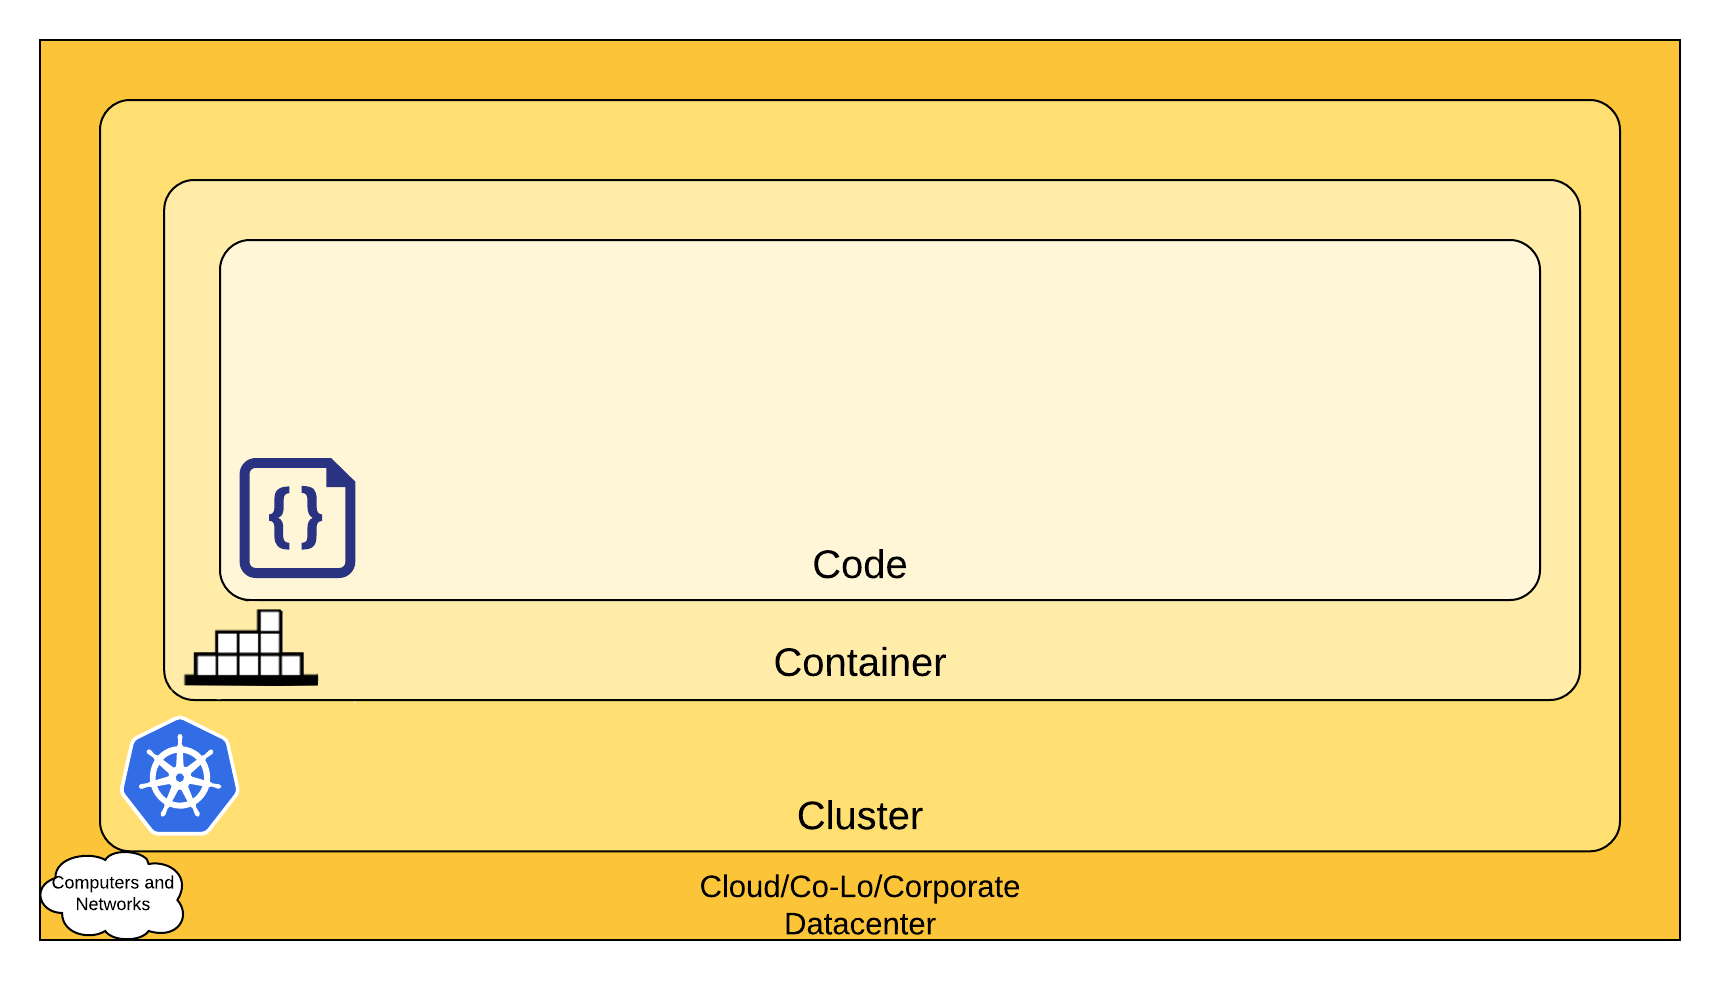
\includegraphics[width=0.8\textwidth]{images/4c.png}
  \caption{The 4C's of Cloud Native security (taken from source \cite{4cs})}
  \label{fig:4cs}
\end{figure}

Although the configuration of the Kubernetes network policies and their intended effect might remain consistent, their result might deviate from the expectations due to changes in the cluster state. Kubernetes pods might be added, updated or removed and depending on the matches between its applied labels and existing \acrshort{np} label selectors this can result in unwanted or missing connections. Even when such unwanted network behaviour gets caught it might be hard to resolve due to the size of the cluster. The scale of this problem increases when we take into account that this same issue can happen when adding, updating or removing Kubernetes network policies or OpenStack security groups and security group rules. Additionally, these different configurations in the separate layers of the 4C's security model can negatively impact each other. We will illustrate this impact with an example.
\\[10pt]

Imagine a cluster with two deployed containers: a web application and a database upon which the web application depends for the data that will need to be displayed. The application manager responsible for the web application knows of this dependency on the database and defines the correct network policies in the cluster layer so that the containers can communicate. What the application manager does not know however is that the person responsible for the \acrshort{vm}s in the cloud layer, who we will call the cloud manager, works according to the principle of least-privilege \cite{leastprivilige}. As a result, the \acrshort{vm}s on which the containers are deployed are prevented from communicating by their networking rules, since they had no reason to communicate before the deployments. We now have a conflict between the cluster and cloud layer which results in an unreachable database container and a non-functioning web application.
\\[10pt]

These types of conflict can easily be overlooked and need to be verified often due to the constantly changing state of a cluster. Additionally, keeping the principle of least privilege enforced while allowing necessary communication gets more complicated as the size of the cluster grows as well. At the moment of writing and to the best of our knowledge there is currently no solution available that detects conflicts in configuration between network rules in the cloud and cluster layer.
\\[10pt]

% ===============================================================
\section{State-of-the-art} \label{sec:stateoftheart}
When looking for solutions for conflict detection of network security rules that include both the cloud and cluster layers we found that existing research solutions often came close, but were always missing at least one essential part. We will briefly describe some of these existing solutions that came closest to the desired properties of conflict detection
\\[10pt]

\textbf{Grashopper} \cite{grashopper}  aims to solve the same problem of misconfigurations between the cloud and cluster layer, but does not use conflict detection. Instead, it will generate the security groups of the cloud layer based on the network policies in the cluster layer. conflicts are thus prevented instead of detected. However, it starts with the assumption that network policies are always correct, called the base truth. We differ from this approach by not having a base truth since the two different layers are managed by separate people and/or instances and their priorities might not align. Since we do not assume a base truth we can not offer a resolution step in this thesis: we can not decide whether the the cloud or the cluster layer is incorrect, only whether or not they are misaligned.
\\[10pt]

\textbf{Kano} \cite{kano} detects inconsistencies in network policies to ensure no redundancy or conflicts exist between them. 
To achieve this Kano generates a square matrix of size \(kxk\) where \(k\ =\ amount\  of\  containers\  in\  the\  cluster\) where a 1 in the position [i][j] means that the pod with index [i] can communicate towards the pod with index [j] respectively. With this matrix as a baseline, it detects various possible misconfigurations due to network policies. However, it does not look at the cluster layer for conflicts and is therefore not extensive enough in its approach. Still, the methods and practices described in the Kano paper, such as the generation of this matrix are a solid base upon which we will build our thesis. We did however find a drawback to the generation method of the matrix: the kanomatrix needs to be fully regenerated after every change in cluster status that might affect it, such as adding or removing a pod or a network policy. With the changing nature of a cluster an incremental approach of updating the kanomatrix instead of fully regenerating it might be more beneficial and could mean an increase in efficiency. For a more in-depth description of Kano, we refer to \autoref{sec:kano}.
\\[10pt]

\textbf{NFVGuard} \cite{nfvguard} is the first solution we found that does multilevel security verification but applies this to the NFV stack. NFV stands for Network functions virtualization and is a way to replace proprietary hardware for network services with virtualized components. In the 4C's of Kubernetes security the NFV stack would be placed within the cloud layer, and thus does not provide conflict detection between cluster and cloud layer. However, some principles can be taken from the NFVGuard approach, such as the collection of relevant security data across the different layers of a stack before verifying their properties. Less interesting for us is how NFVGuard turns the collected data into \acrfull{fol} properties after which they use existing Constraint Satisfaction Problem (CSP) solvers. This approach makes sense in the very differing layers and data sources of the NFV stack but would introduce too much overhead in our solution. The different network security rules between the cluster and cloud layer are more straightforward in their correlation and promise to allow a more direct comparison without translation to \acrshort{fol}.
\\[10pt]

\textbf{TenantGuard} \cite{tenantguard} verifies network isolation between different tenants in the same cloud environment. Their solution promises to be scalable by using an incremental approach to keep the computation time low. However, it does not provide isolation between the cluster and cloud layer, but only within the latter of the two. Fortunately, Tenantguard does use some techniques that will be useful in our implementation such as the use of tree-based data structures for quick data retrieval, and most of all an incremental approach. Tenantguard identifies all events on the cloud that influence isolation and will trigger an update of its conflict evaluation based on these events. It will only look at the parts of the isolation that are influenced by this specific event instead of recalculating the conflicts for the entire cluster, decreasing the computation time. In this thesis, we will use a similar event-driven incremental approach.
\\[10pt]

\textbf{Microsegmentation tools} leverage the principle of least privilege \cite{leastprivilige} and zero trust \cite{trust} to prevent conflicts from existing, effectively making conflict detection redundant. Some notable examples of microsegmentation tools are Paloalto's PrismaCloud \cite{prismacloud}, Illumio core \cite{illumio}, cisco ACI \cite{ciscoaci} and VMWare NSX \cite{vmwarensx}. The goal of these tools is to limit the possibility of a malicious attack spreading through a cloud stack by hindering lateral movement. To do this it leverages network rules that limit connections to the minimum required for normal operation. Although this does prevent conflicts within these network rules an essential part is missing in all these microsegmentation solutions: they do not orchestrate these network rules across different layers in the cloud stack. Therefore conflicts can  still exist between the cloud and cluster layer, even when these tools are correctly applied 

% ===============================================================
\section{Goals} \label{sec:goals}
As mentioned in the previous section there is a gap in current state-of-the-art technologies for detection of conflicts in network rules through the cloud and cluster layer. Our goal is to fill this gap with an algorithm that monitors a cluster for changes in network policy and pod configurations upon which it will start conflict detection between communication states of Kubernetes pods and OpenStack instances. Our algorithm is incremental in the sense that it constantly monitors the cluster layer for events that might change communication between components after which it will update the stored cluster state with that specific event. This new cluster state will then be used to detect new conflicts. Events in the cloud layer might affect conflicts as well but are out of scope for this thesis. Additionally, the algorithm offers a startup detection that will find any existing conflicts upon execution of the algorithm to ascertain whether or not the starting cluster state is conflict-free.
\\[10pt]

With this algorithm, we want to guarantee that all misconfigurations between the cloud and cluster layer are detected and reported in a timely fashion. We hope to provide conflict detection that is faster than the time it takes for the changes of the triggering event to become effective in the cluster. Additionally, we want to check any affected components for redundancy upon events that decrease the number of connections in the cluster, such as network policies that have become redundant because their only matching pod got removed. This ensures that no redundant components are left to be forgotten, which could otherwise open up new attack vectors.
\\[10pt]

The main application strategy for our algorithm is two-fold: It could be integrated into a scheduler to guarantee that proposed pod placements do not introduce conflicts, or it could be used as a verification tool that constantly monitors for conflicts or is periodically executed so that operators know at which components to look to find and resolve conflicts.


% ===============================================================
\section{Approach } \label{sec:approach}
The approach of this thesis is split up into the following steps:
\begin{itemize}
    \renewcommand{\labelitemi}{\scriptsize$\blacksquare$}
     \item A literature study of the current technologies around container orchestration, cluster security and conflict detection.
    \item Defining a problem statement and scope for the thesis
    \item researching possible solution approaches to the problem statement and creating a first pseudo-code algorithm. Afterwards, we research capable data structures and coding practices to enable the creation of the algorithm.
    \item Implementation of the algorithm using an iterative approach.
    \item evaluating the final algorithm with the following research questions:

    \begin{enumerate}
        \item[--] What is the difference in time cost between an incremental update of the Kano matrix compared to newly generating the Kano matrix for every event and how does this difference scale with pod/policy numbers
        \item[--] What is the difference in space cost between an incremental update of the Kano matrix compared to newly generating the Kano matrix for every event and how does this difference scale with pod/policy numbers
        \item[--] What is the relationship between pod/policy numbers and the time cost of conflict detection?
        \item[--] What is the relationship between pod/policy numbers and the space cost of conflict detection?
    \end{enumerate}
\end{itemize}


% ===============================================================
\section{Text overview} \label{sec:textoverview}
We will now describe how the remainder of the chapters is divided. In chapter 2 we will give background information about technologies that will be used within this thesis. We continue with chapter 3 which will describe our solution for conflict detection with the help of pseudo-code descriptions of our implementation. chapter 4 is where we will evaluate our algorithm based on the four earlier-mentioned research questions by executing two main experiments. Lastly, chapter 5 will provide a conclusion to this thesis as well as some self-reflection.
\cleardoublepage


\newpage
\chapter{Background}                                 \label{ch:background}
This chapter aims to give some background information about concepts and technologies related to the thesis.
We will start talking about Containers and their advantages, after which we talk about how to run these containers using a container engine, specifically Docker Engine. The third section will talk about the container orchestration software Kubernetes and it's network policies. After this the focus shifts to Kano: a system to cover container network policy verification. Lastly we will talk about the cloud operating system Openstack and its network security solutions.


% =========================================
\section{Containers}
Deploying an application on a cloud computing infrastructure or platform is not an easy task: Even though the application might work perfectly when locally developed and tested it is not guaranteed to work in a cloud environment due to possible differences in Operating System (\acrshort{os}) or hardware settings. Luckily this problem can easily be solved by creating a virtual machine (\acrshort{vm}) with the same \acrshort{os} and hardware settings as the local developing environment, which is called a hypervisor deployment \cite{Bernstein2014}. However, such a hypervisor deployment also has its drawbacks: A \acrshort{vm} often has more functionality than the application strictly requires, such as access control and user management. This in turn decreases scalability since the \acrshort{vm} files increase the size of deployments, causing slower deployment, deletion and rebooting times.
\\[10pt]

A solution for these limitations is using containers instead. with containers, applications share an operating system with each other when deployed on the same host server, meaning a decrease in size compared to a fully fledged \acrshort{vm} environment for each application. Additionally, containers allow quicker deployment, deletion and rebooting then the hypervisor alternative since they offer a limited number of services. Containers are therefore more flexible in scalability according to the elasticity of demands.  these differences between hypervisor and container deployments are shown in \autoref{fig:compdeployment}. 
\\[10pt]

But this is not the end of the story, since without an industry standard around containers they would not be deployable on any hosts, nor be portable and scalable. To support this effort of creating industry standards  the \acrfull{oci} \cite{OCI} was introduced by the Linux Foundation \cite{linuxfoundation}. \acrshort{oci} dictates in 3 specifications how to standardize your application so that it can be deployed in a container \cite{opencontainers}. The first step in achieving containerized deployment is packaging the application into an image format. if this image is made according to the \acrshort{oci} image format specifications it will define all necessary information for the launch of the application on a specified platform, such as environment variables and application arguments. To facility the sharing of these images public and private registries can be utilised, which follow the \acrshort{oci} distribution specifications.
\\[10pt]

Almost all mainstream players in the industry support and follow these \acrshort{oci} guidelines, effectively creating a strong standard in the industry with many benefits as result. For example, outsourcing cloud management to public providers enables lower cost due to economy of scale, where the location cost of the servers is divided between all the user that run their applications on these servers. If you want to use these public providers you often only need to create and share your image. Changing providers for your deployment is also fairly easy thanks to this industry standardization, making for a competitive market. Furthermore the portability of container images allow for quick deployments, compared to hypervisor deployments which require more manual configuration. 
\\[10pt]


\begin{figure}[htbp]
  \centering
  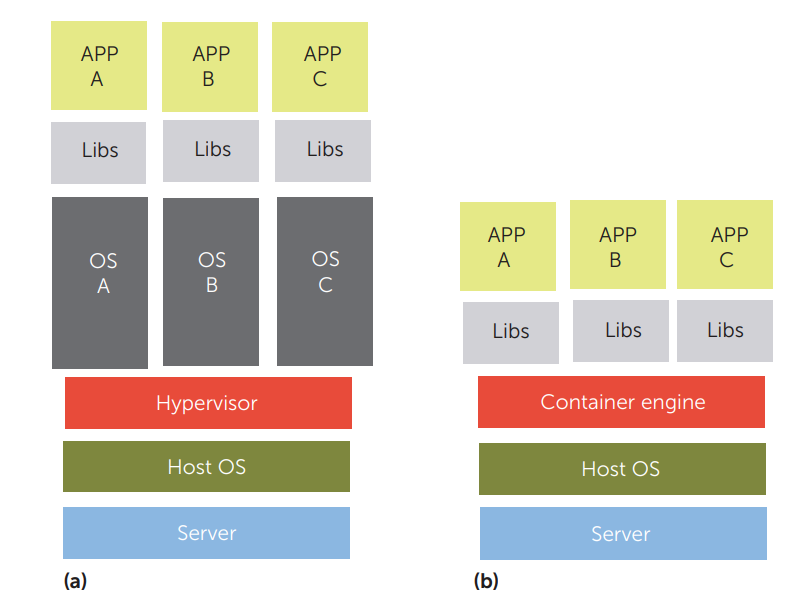
\includegraphics[width=0.8\textwidth]{images/bernstein-hypervisor-vs-container-deployment.png} 
  \caption{Comparison of (a) hypervisor and (b) container-based deployments (taken from source \cite{Bernstein2014})}
  \label{fig:compdeployment}
\end{figure}


% ===========================================
\section{Docker Engine} \label{sec:containerruntime}
Once an \acrshort{oci} standard image is created for an application and is stored in a registry it still needs to be deployed as a container. We previously talked about cloud providers, but even they need a way to turn the image into a running container. This is where container engines such as Docker Engine come into play \cite{dockerengine}. Container engines are the bridge between the end-user and the deployment of a container based of an image: they accept user requests and pull the images from the registry to finally run the container based on the metadata in the image. It also offers an API so the engine can be called by a higher abstraction layer such as Kubernetes (see \autoref{sec:kubernetes}). 
\\[10pt]

Container engines such as Docker engine not only run containers, but also manage dependencies and allow multiple containers to run on the same \acrshort{os} by using virtualization while keeping different applications separated for security reasons \cite{cnwiki}. \autoref{fig:deployment} shows an example of the usage of Docker Engine for a deployment of 4 containers that together provide 2 different services (S1 and S2). The engine itself only installs the required binaries and libraries for the containers as described in the image, and shares these between all the containers requiring them. This saves on resources and improves booting speed since binaries and libraries only need to be loaded once.
\\[10pt]

\begin{figure}[htbp]
  \centering
  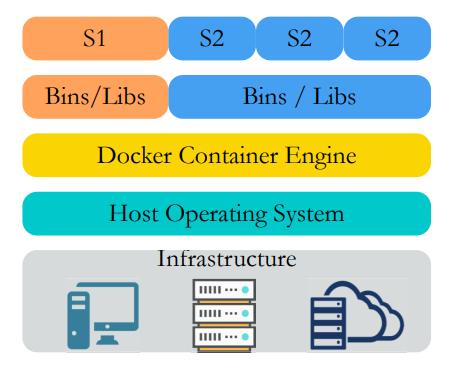
\includegraphics[width=0.4\textwidth]{images/docker-containers.png} 
  \caption{a container deployment using Docker Engine (taken from source \cite{resman})}
  \label{fig:deployment}
\end{figure}

Docker Engine is owned by Docker \cite{docker} and is a pure container engine without any further bells and whistles. If more functionality is required such as a load balancer, integration with Docker Compose or image vulnerability scanning then Docker Desktop should be considered \cite{comparisonenginevsdesktop}. In this thesis we will not be using Docker Desktop, but an alternative container orchestration tool called Kubernetes (see \autoref{sec:kubernetes}). Kubernetes also builds directly on Docker Engine, therefore we will now look at Docker Engine's inner working.
\\[10pt]

If we delve a bit deeper into the development of Docker Engine we find that it is an open source project supported by the Moby community \cite{moby}. Moby is a framework that consists of multiple plug-and play components that enable you to manage images, configuration and secrets, while providing networking  and provisioning to your container, as seen in \autoref{fig:moby}. Docker engine thus offers some extra functionality for managing a container thanks to the Moby framework, but underneath the shell it in turn relies on a container runtime to actually run its containers.
\\[10pt]

\begin{figure}[htbp]
  \centering
  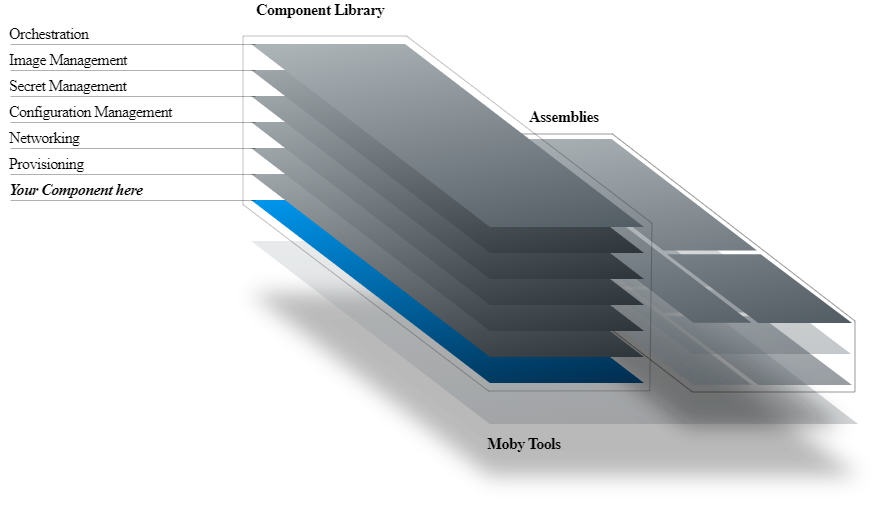
\includegraphics[width=0.8\textwidth]{images/moby.png} 
  \caption{Moby framework (taken from source \cite{moby})}
  \label{fig:moby}
\end{figure}

 Container runtimes manage the life-cycle of containers and serve as the bridge between the host system and the container \cite{containerterminology},\cite{contruntime}. when a container runtime is requested to run a container it will first pull the correct image from its image repository and will then ready the host system based on the metadata included in that image. This includes  giving the container network attachments and storage if required. Afterwards it will communicate with the kernel to start the container. container runtimes adhere to \acrshort{oci}'s runtime specifications which means they are interchangeable with many alternatives such as containerD \cite{containerd}, CRI-O \cite{crio} and Mirantis \cite{mirantis} on the market. Our container engine, Docker Engine, is designed specifically with containerd in mind which makes it our obvious choice as container runtime.
\\[10pt]



% =========================================
\section{Kubernetes}\label{sec:kubernetes}

Even though Docker Engine can easily deploy multiple containers, managing all of them can become challenging very quickly, especially as the size of your container cluster scales up to possibly hundreds or thousands of containers. Issues such as container crashes, loss of network connectivity, running out of resources and many more can arise and need to be dealt with correctly. To help solve these challenges container orchestration tools were introduced such as Docker Swarm \cite{dockerswarm}, Apache Mesos \cite{apachemesos}, and the current industry standard Kubernetes \cite{resman} \cite{CNCFSurvey}. This thesis will research and utilise Kubernetes.
\\[10pt]

\acrfull{k8s} is an open-source platform that automates container orchestration whether it is for one, hundreds, or even thousands of containers, and is supported by most major public cloud providers such as \acrfull{aws} \cite{aws}, Microsoft Azure \cite{azure} and \acrfull{gcp} \cite{gcp}. Kubernetes automates functionalities such as scaling, deployment, storage, rollbacks, load balancing, secret management and many more, all of which can be configured using specifications created by a cluster manager in YAML or JSON format. To have a better understanding Kubernetes \autoref{fig:kubernetes} shows an overview of K8s components, where they are typically deployed and how they communicate with each other in a cluster. In the rest of this section we will describe the Kubernetes components and concepts in the figure that are important for this thesis. 
\\[10pt]
\begin{figure}[htbp]
  \centering
  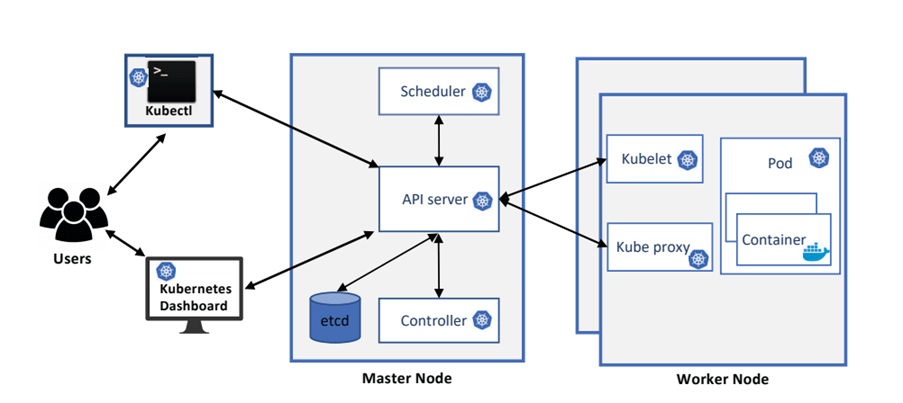
\includegraphics[width=0.8\textwidth]{images/kubernetes-structure.png} 
  \caption{a brief overview of Kubernetes (taken from source \cite{IslamShamim2020a})}
  \label{fig:kubernetes}
\end{figure}

\textbf{Node:} \label{comp:node} Nodes are the biggest component in a \acrshort{k8s} cluster and have two variations which are not mutually exclusive: worker and master nodes. They are machines, either virtual or physical, on which containerized applications run. Worker nodes host \hyperref[comp:pod]{pod(s)}, a \hyperref[comp:kubelet]{kubelet service} and a kube-proxy service. Master nodes on the other hand are part of the control plane, and are responsible for managing the worker nodes. They host components such as the controller,scheduler, \hyperref[comp:apiserver]{API server} and etcd storage. These control plane components can be spread across multiple master nodes to provide fault-tolerance. Each cluster needs at least one node to operate correctly but can easily scale up to thousands.  \cite{node}
\\[10pt]

\textbf{Pod:} \label{comp:pod} Pods are the smallest deployable computational components in a \acrshort{k8s} cluster, run on a specific \hyperref[comp:node]{node}, and house one or more containers that are tightly coupled. A pod remembers trough its specification file how to run the container(s) it is responsible for and shares storage and network resources between them. If containers are tightly coupled they can run on a single pod to have unrestricted communication and shared resources, but this introduces some security concerns such as the possibility of malware spreading between those containers. Duplicates of containers can be deployed on separate pods  in order to increase an application's workload (horizontal scaling). To redirect requests to an application without any noteable differente for the end-user the load-balancer is introduced. It will automatically redirect requests to the application with the least current tasks to assure optimal spreading of end-users. Alternatively to horizontal scaling the available resources for a pod can be increased (vertical scaling) to scale workload capabilities. \autoref{fig:pod} shows an example of a pod specification in the form of a YAML file. \cite{pod}
\\[10pt]

\begin{figure}[htbp]
  \centering
  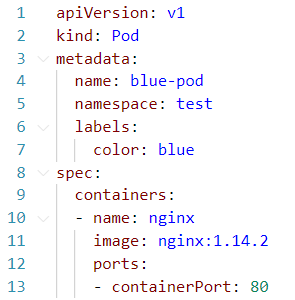
\includegraphics[width=0.5\textwidth]{images/pod.png} 
  \caption{an example pod specification}
  \label{fig:pod}
\end{figure}

\textbf{Kubelet:} \label{comp:kubelet} Each node in a cluster runs its own kubelet service component. The kubelet manages all the \hyperref[comp:pod]{pods} on the \hyperref[comp:node]{node} it is deployed on by deploying, monitoring and deleting \hyperref[comp:pod]{pods}. It knows how to deploy these pods thanks to the PodSpec YAML or JSON file it receives from the \hyperref[comp:apiserver]{API server} in the control plane. By using the kubelet Kubernetes can ensure \hyperref[comp:pod]{pod} crashes get noticed and handled according to specifications. \cite{kubelet}
\\[10pt]

\textbf{API server:} \label{comp:apiserver} The Kubernetes API Server offers REST operations trough which users can interact with the cluster. It takes user inputs from the command line interface Kubectl or from a Kubernetes dashboard and communicates the necessary changes to the other components. It also validates request and configures the data that passes trough it. Libraries have been built on top of the REST operations to facilitate new ways to interact with the api server, and for this thesis we shall be using the python Kubernetes library as the main method of communication with the cluster \cite{pythonk8s} \cite{kubeapiserver}.
\\[10pt]


\textbf{Namespace:} \label{comp:namespace} A namespace is a mechanism to separate groups of resources in a Kubernetes cluster. Within a namespace each resource must have a unique name, but equal names can exist in different namespaces. objects that are used cluster-wide, like a \hyperref[comp:node]{node} for example, do not allow the specification of a namespace. An example usage for a namespace would be the separation of different tenants according to their subscription plan on the cluster's resources \cite{namespace} \cite{feasability}.
\\[10pt]


\textbf{Labels:} \label{comp:label} Labels are key/value pairs which allow us to identify objects such as pods and network policies. Multiple labels can be applied to a single object, much like a \acrfull{rbac} system where roles are linked to users \cite{rbac}. Important to note is that for each object there can be no duplicate keys. e.g. applying \textit{role: database} and \textit{role: application} to a single object is not allowed and will result in errors. In the previously mentioned \autoref{fig:pod} we can see an example of a Kubernetes \hyperref[comp:pod]{pod} that has the label \textit{color: blue} attached to it. 
\\[5pt]

In order to retrieve all objects based on labels the use of label selectors are required.  If multiple labekl requirements are specified in a label selector then the found objects will have to match with not one but all of these requirements. Furthermore there is a difference between equality-based requirements and set-based requirements. When using the first matching objects must satisfy the (non)-equality with a specific label, e.g. it must (not) have the label \textit{role: db}. The set-based requirement on the other hand offers three choices to be used with a set of values: \textit{in}, \textit{notin} and \textit{exists}. An example of a set-based requirement would be \textit{role in (database, application)} where either \textit{role: database} or \textit{role: application} would fulfil the requirement. \autoref{fig:np} shows an example of equality based-requirements in a network policy. \cite{labels}
\\[10pt]

\begin{figure}[htbp]
  \centering
  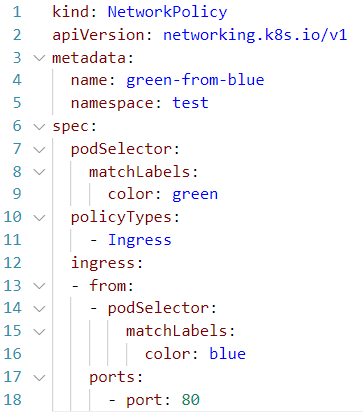
\includegraphics[width=0.5\textwidth]{images/np.png} 
  \caption{an example network policy specification}
  \label{fig:np}
\end{figure}


\textbf{Network policy:} \label{comp:networkpolicy} A \acrfull{np} is used to control network traffic on the IP address or port level. Network policies are applied only to pods, but can use different type of selectors: a namespace selector will just target all pods in the defined namespace, an ipBlock selector targets pods based on a match in IP, and lastly pod selectors target based on labels. This last option will only look at pods with matching labels in the same namespace in which the \acrshort{np} is deployed. In this thesis we only focus on pod selectors with labels and work in a single namespace.
\\[10pt]
To describe the general build of a network policy we will look back at \autoref{fig:np}. We can see that the \acrshort{np} is in the namespace \textit{test} and that it selects pods that have the label \textit{color: green}. This \acrshort{np} will thus only apply to pods in the namespace test with the same label. There are two types of policies: Ingress policies that define from which pods communication is allowed and egress policies that define to which pods communication is allowed. Thus the example \acrshort{np} in \autoref{fig:np} specifies that all pods with the label \textit{color: green} in the namespace test are allowed to accept communication from all pods with the label \textit{color: green}.
\\[10pt]


Important to note is that this does not mean pods with the label \textit{color: blue} are allowed to send messages to pods with the label \textit{color: green} yet. For this we need a correctly defined egress rule as well. In practice at least two network policies are required for pods to communicate. \cite{k8snp}



% =========================================
\section{Kano}\label{sec:kano}
Although network policies offer extra security for a Kubernetes cluster it also has its drawbacks. They need to be closely managed to ensure no contradictions are specified and that containers can connect to other container they rely upon. To combat these difficulties Kano was introduced by researchers at the Tsinghua University in Bejing.
\\[10pt]
Kano is a container network policy verification tool presented in 2020 that, to quote the authors, solves the following problem: "In a container network, do the network
policies violates the network constraints?" \cite{kano}. It does so by creating a matrix representing the container connections based on the defined network policies. Once this matrix is created it is leveraged to find underlying issues such as redundant \acrshort{np}s or an isolated container and those issues are reported to the user. We will continue to explain Kano in more detail since the solution algorithm of this thesis builds directly on some of Kano's concepts.
\\[10pt]

\textbf{Kano Reachabilitymatrix:} \label{kano:matrix} Kano starts by modelling a container network as a bipartite graph where the vertices are containers with 2 sets of edges \textit{E1} and \textit{E2}: ingress and egress network policies respectively. \autoref{fig:kano-bipartite-graphs} depicts this, but in 2 bipartite graphs instead of one to easily separate between the ingress and egress sets. The intersection of these sets  ($\textit{E1} \cap \textit{E2}$) represents connections between connections allowed by both an ingress and an egress rule. In order to save storage space and to allow quicker computations Kano does not actually save the container network as a bipartite graph, but as a matrix with bit arrays as rows, which we will call the kanomatrix or reachability matrix from now on. The kanomatrix is a square matrix of size \(kxk\) where \(k\ =\ amount\  of\  containers\  in\  the\  cluster\). A 1 in position [i][j] means that the container with index [i] can communicate towards the pod with index [j] respectively. \autoref{fig:kano-reach-matrix} shows the ingress and egress matrix that correspond to the bipartite graphs in \autoref{fig:kano-bipartite-graphs}, as well as the final kanomatrix which is equal to the intersection of the two matrices, achieved by using the bitwise AND operation between the matrices' bit arrays.
\\[10pt]
\begin{figure}
\centering
    \begin{minipage}[b]{0.8\linewidth}
        \centering
        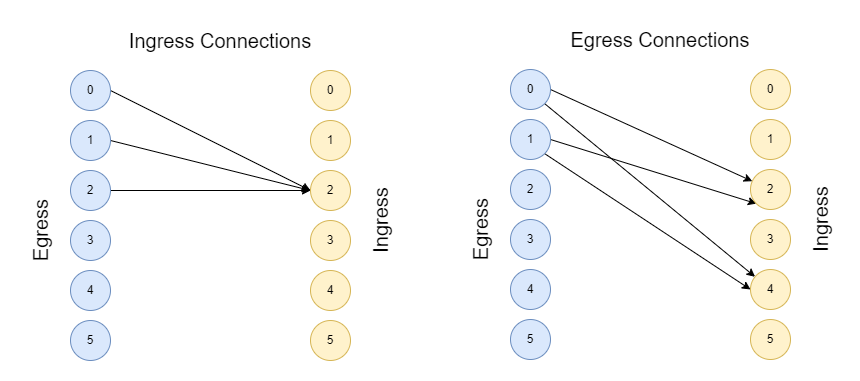
\includegraphics[width=0.8\textwidth]{images/kano-combined-connections-graph.png} 
        \caption{Bipartite graphs for Kano matrix generation} 
        \label{fig:kano-bipartite-graphs}
    \end{minipage}
    \begin{minipage}[b]{0.8\linewidth}
         \centering
          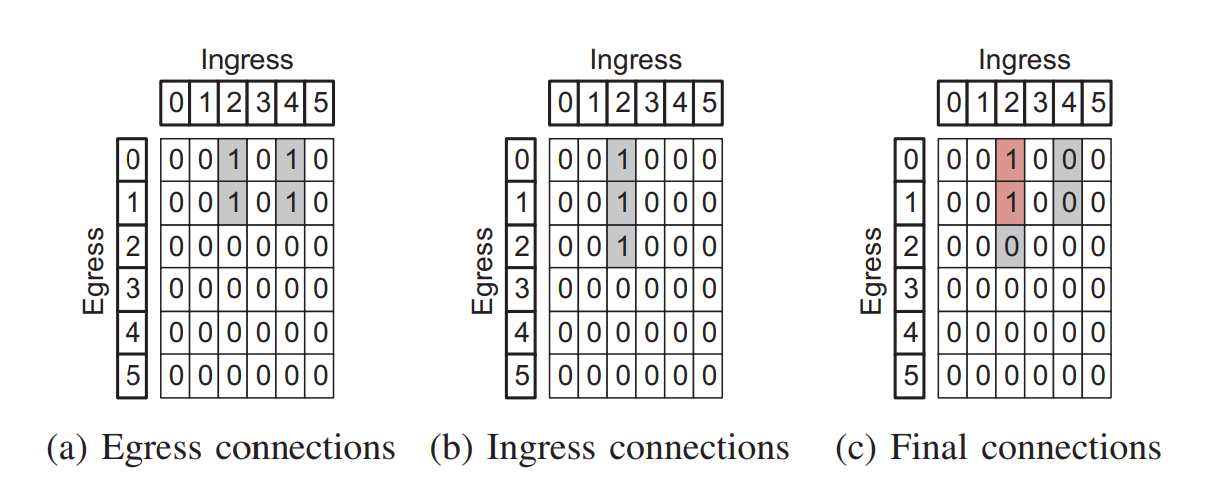
\includegraphics[width=0.8\textwidth]{images/kano-matrix-generation.png} 
          \caption{Container network reachability matrix model (taken from source \cite{kano})} 
          \label{fig:kano-reach-matrix}
    \end{minipage}
      
\end{figure}

\textbf{Prefiltration algorithm:} \label{kano:prefiltration} In a container cluster changes happen frequently and therefore the reachability matrix often needs updating. A naive solution to update the reachability matrix would be to iterate over all policies and match them with containers with corresponding labels. This solution is not scalable to execute for every change since the time complexity would be $O(mn)$ with $m\ =\ number\ of\ policies$ and $n\ =\ number\ of\ containers$. To counter this Kano introduced a prefiltration algorithm based on bit arrays. The algorithm start by creating a hashmap, where each key is a label that is applied to at least one container, and the values are bit arrays with a length equal to the amount of containers in the cluster. In such a bit array the position of a set bit represents that the container with its index equal to the position has the corresponding label key applied. This is seen in \autoref{fig:kano-cont-prefiltration}.
\\[10pt] 

When searching to which containers a network policy applies we simply find the bit arrays corresponding to the selector labels of a policy in the hashmap. By applying a bitwise AND to these bit arrays we get a bit array with bits set for each container that matches all labels from the policy. This is illustrated in \autoref{fig:kano-pol-prefiltration}. The time complexity of creating the hashmap based on the containers is $O(m)$, while the lookup for a policy is $O(1)$, which is a drastic improvement on the naive solution.
\\[10pt]

\textbf{Violation check:} \label{kano:violationcheck} Once the reachability is created with the prefiltration algorithm it can be used to verify some violations. The following descriptions are taken directly from the Kano paper \cite{kano}:
\begin{itemize}
    \renewcommand{\labelitemi}{\scriptsize$\blacksquare$}
    \item \textit{All reachable:} A container can be reached by all containers.
    \item \textit{All isolated:} A container cannot be reached by any container.
    \item \textit{User cross:} A container can reach other user’s container in the container network.
    \item \textit{Policy shadow:} The connections built by a policy are completely covered by another policy, then this policy may be redundant
    \item \textit{Policy conflict:} The connections built by a policy are totally contradict the connections built by another.
\end{itemize}
Additionally, you can define your own constraints with the use of a declarative language, for example to guarantee two containers are able to communicate. Since the violation checker will not be used in this thesis we will not go into detail about its implementation
\\[10pt]

\begin{figure}[htbp]
  \centering
  \begin{minipage}[b]{0.45\linewidth}
    \centering
    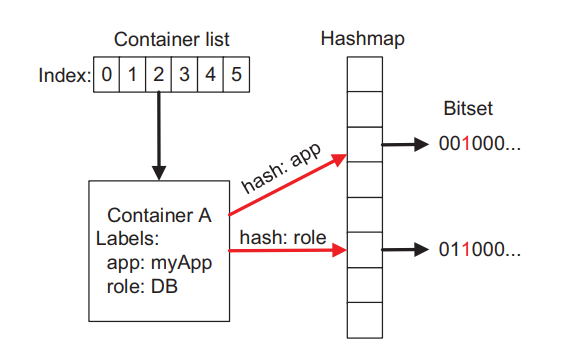
\includegraphics[width=\textwidth]{images/prefil_cont_labels.png}
    \caption{Prefiltration of container labels (taken from source \cite{kano})}
    \label{fig:kano-cont-prefiltration}
  \end{minipage}
  \quad % Add some horizontal space between the subfigures
  \begin{minipage}[b]{0.45\linewidth}
    \centering
    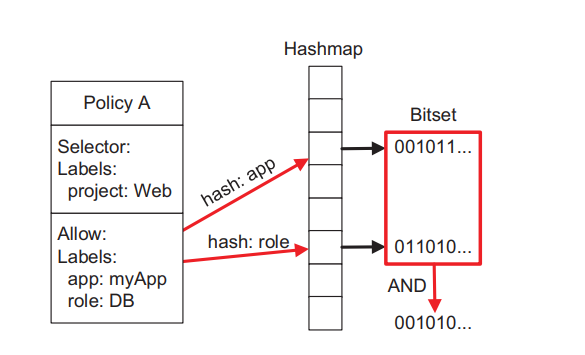
\includegraphics[width=\textwidth]{images/prefil_pols.png}
    \caption{Prefiltration of policies (taken from source \cite{kano})}
    \label{fig:kano-pol-prefiltration}
  \end{minipage}
\end{figure}


% =========================================
\section{Calico}\label{sec:calico}

Pods, and by extension containers, In a Kubernetes cluster are not able to communicate with each other by default. Instead you need to either explicitly create links between the pods or give each pod its own unique IP address within the cluster. The latter option of two is called the Kubernetes network model, and to achieve it a \acrfull{cni} plugin is required. \cite{k8scni} \cite{k8snetworkmodel}. The \acrshort{cni} is a specification for writing plugins that should only be concerned with network connectivity of containers and deleting these as the container gets removed \cite{cni}. Many plugins based on the \acrshort{cni} project exist, such as Weave \cite{weave}, Cilium \cite{cilium} and Project Calico \cite{calico}.
\\[10pt]

There are some rules that Kubernetes set to which \acrshort{cni} plugins must adhere before being allowed into the ecosystem. First and foremost pods must be able to communicate with each other, independently of the node on which they are deployed without the necessity of \acrfull{nat}. Secondly all Kubernetes components on a node such as the kubelet and kube-proxy must be able to communicate with all pods on that node. Together these 2 rules guarantee that \acrshort{cni} plugins do not hinder the working of the Kubernetes cluster, but still allow freedom for addition of functionalities.
\\[10pt]

Calico has been chosen for this thesis to ensure ready-to-go communication between the containers for testing purposes. Calico offers specific optimisations for Kubernetes by using eBPF, a Linux kernel feature that allows you to run a \acrshort{vm} inside the kernel itself \cite{ebpf}. This means that Calico does not have to rely on the default iptables based Linux standard for network routing and was able to improve latency and performance with its own solutions. Calico also enforces the Kubernetes network policies and, although not used in this thesis, offers its own kind of network policies on top of the default \acrshort{k8s} ones if required. The last reason we choose Calico instead of one of the alternatives is the default support for VM networking with Openstack, thanks to the Neutron ML2 plugin \cite{neutron}. 


% =========================================
\section{Openstack}\label{sec:openstack} In order to host our nodes in a Kubernetes cluster we have two options: Using physical devices or \acrlong{vm}s. The second option not only reduces overhead, but requires no extra physical hardware if your existing hardware has enough resources, and can thus be scaled easily according to the needs of the cluster. Just like physical machines \acrshort{vm}s need to be managed, and this is where virtual operating systems come into play, often synonymously called cloud operating systems due to cloud native computing becoming the standard \cite{CNCFSurvey}. Some examples of cloud operating systems are Google Chrome OS \cite{chromeos}, \acrshort{aws} \cite{aws} and Openstack, which is our choice for deploying our \acrshort{vm}s in this thesis \cite{Openstack}.
\\[10pt]

Openstack automates the managing of computing and network resources for clusters of physical and virtual machines, which can be easily directed trough the dashboard application or directly via the API's. Openstack has great modifiability by allowing cluster administrators to select the components of their choice with example categories such as hardware life-cycle, storage, orchestration and application life-cycle. This way Openstack can be expanded to the requirements of the cluster. A \acrshort{vm} deployed with OpenStack is called an instance, and in this thesis Openstack is used to deploy instances that serve as Kubernetes nodes. Openstack also has its own network security solutions to manage connection between instances, which we will more in depth in the following paragraphs.
\\[10pt]

\textbf{Security Groups}\label{sec:securitygroups} Security Groups (\acrshort{sg}) are a way to group network security rules together to be easily applied to instances within the Openstack cluster. They are identified by their name, which must be unique within the cluster, and can carry a description to describe its intended usage. Every instance has the $default$ security group applied if no custom \acrshort{sg} are linked. This default security group denies all incoming traffic and allows only outgoing traffic to your instance. A limit can be imposed on the maximum rules per security group and on the maximum defined security groups in the cluster by the security groups quota. \cite{sg} \cite{sgquotas}
\\[10pt]

\textbf{Security Group Rules}\label{sec:securitygrouprules} Security group rules are essentially IP filter rules to allow or block communication from certain IPs. These rules also specify a protocol for which they are applied, with the choices being TCP, UDP or ICMP. When wanting to target multiple protocols multiple security group rules are needed. The IP or IP range on which the rule applies must be specified in CIDR notation and a port range can be included as well. Alternatively to selecting IPs another security group can be targeted instead, with the advantage that instances can be added or removed from security groups without the need for revision of the security group rules. \autoref{fig:sgrule} shows a security group wit the name $open$ that holds two security group rules, one for UDP and one for TCP but both selecting all possible IPs and ports (65535 being the highest value of an unsigned 16-bit integer and thus the highest possible port value). \cite{sgrule}
\\[10pt]

\begin{figure}[htbp]
  \centering
  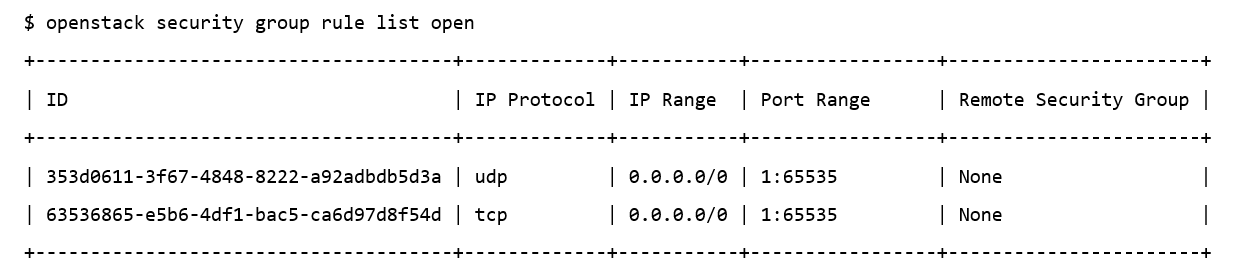
\includegraphics[width=\textwidth]{images/sgrule example.png} 
  \caption{Security group rule example (taken from source \cite{sg}}
  \label{fig:sgrule}
\end{figure}

\cleardoublepage


\newpage
\chapter{Proposed Solution}                                 \label{ch:solution}

In this thesis, we aim to create an algorithm that, once running on one of the control plane nodes of a Kubernetes cluster, continuously watches the state of that cluster and detects any conflicts between cloud and cluster layer. To achieve this We capture the six types of events in the cluster that can influence the connection between containers in the cluster layer as seen in \autoref{tab:events}. When one of these events is captured an automatic conflict detection should be triggered and the algorithm must report on all possible conflicts between the cloud and cluster layer. It should be noted that changes in the cloud layer can influence connections as well (e.g. security groups being created) but that this is outside the scope for this thesis.
\\[10pt]
\begin{table}[htbp]
  \centering
  \begin{tabular}{|c|c|}
    \hline
    pod & network policy \\
    \hline
    create & create \\
    delete & delete \\
    update & update \\
    \hline
  \end{tabular}
  \caption{watcher events}
  \label{tab:events}

\end{table}

In order to work incrementally we want to store all necessary information about the current state of the cluster. With this information we can look directly at the relevant containers and network policies for each event and reduce the computation time per event. For example, there is no need to check containers that are not affected by a newly created network policy. We call this the incremental approach, since it incrementally updates the stored cluster state with each event. As a bonus we added a simple startup detection method that can detect conflicts upon startup of the algorithm. periodically running this startup detection could serve as an alternative in case a continuously running algorithm would prove unviable in any way.  
\\[10pt]

We will only monitor a single namespace when executing the algorithm, which can be specified as an argument. The reasoning behind this decision is that the main purpose of namespaces is to isolate groups of resources within the cluster and conflicts between multiple namespaces should thus not exist when used correctly \cite{namespace}. If required multiple instances of the algorithm can be run for different namespaces. We would also like to note that we will deploy only one container per pod in our algorithm, and that therefore the term pod and container might frequently be used as synonyms in the case of variables.
\\[10pt]

In the rest of this chapter We will describe our solution, implemented in Python, that meets all the requirements and solves the problem of conflict detection between cloud and cluster layers. The implementation is based on a Kubernetes cluster with nodes deployed on an Openstack installation. \autoref{fig:algorithm} demonstrates how the algorithm is split up in separate parts, which correlates directly to different python files with the corresponding name and functionalities. We briefly summarize these functionalities for each component of the algorithm before describing them more in depth:
\begin{itemize}
    \renewcommand{\labelitemi}{\scriptsize$\blacksquare$}
    \item \textit{Watcher:} The watcher initializes the other components and leverages the Python Kubernetes library to continuously monitor for each of the six events described in \autoref{tab:events}, which it will forward to the analyzer.
    \item \textit{Analyzer:} The analyzer orchestrates the handling of events passed by the watcher. First these events must be forwarded to the parser to be turned into usable objects. Afterwards the analyzer calls the \acrshort{kic} to update the reachability matrix and cluster state and the \acrshort{sgic} to look at this updated reachability matrix for conflicts.
    \item \textit{Parser:} The parser turns the event data from the watcher into objects that can be used by the Analyzer. Since it's functionality is straight forward this component will not be described in depth in the rest of this chapter.
    \item \textit{\acrfull{kic}:} The \acrshort{kic} handles the incremental update of the reachability matrix and stores all information about the cluster state.
    \item \textit{\acrfull{sgic}:} The \acrshort{sgic} generates a randomised set of security groups and corresponding rules and binds them to nodes upon startup. Additionally it performs conflict detection between the cluster and cloud layer.
    \item  \textit{Model}: The model defines data structures to be used within the other components. These data structures are often created by the parser out of event data, such as Container, Policy and Reachabilitymatrix objects. Finally it leverages the Kano generation method to create a reachability matrix upon startup which offers the base matrix which we update incrementally with each captured event.
    \item  \textit{LabelTree}: A labelTree is a custom tree-like data structure used to store network policies by their selector labels, for quick retrieval by the \acrshort{kic} later on.
\end{itemize}
\begin{figure}[htbp]
  \centering
  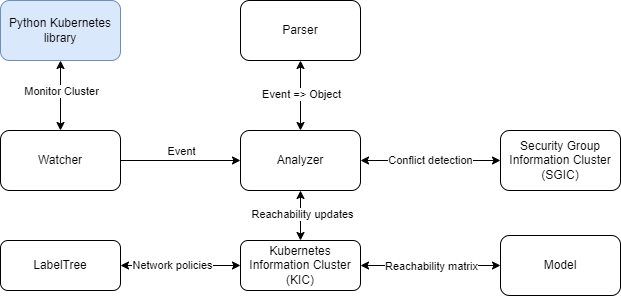
\includegraphics[width=0.8\textwidth]{images/algo-components.png}
  \caption{Algorithm structure}
  \label{fig:algorithm}
\end{figure}



% ==============================================
\section{Model} \label{impl:model} There are many data structures used in the algorithm, most of which are stored in the model file. To ensure a good understanding of these underlying structures in the other components we will first describe the ones that occur most often: the Policy, Container, Store and ReachabilityMatrix.
\\[10pt]

\textbf{Policy:} The Policy structure stores multiple variables which often are specific data structures on their own. We will not describe each of these sub-structures in depth, but instead briefly explain the most important variables in a short manner:
\begin{itemize}
    \renewcommand{\labelitemi}{\scriptsize$\blacksquare$}
    \item \textit{name:} Stores the name of the policy. Although they are not enforced to be unique in the algorithm they will be in practice, since all objects in the same namespace must have unique names. 
    \item \textit{selector:} This data structure stores the labels which selects the grouping of pods to which the policy applies.
    \item \textit{allow:} This data structures stores the labels that select the ingress sources or egress destinations.
    \item \textit{direction:} The direction is a boolean that indicates weather it is an ingress (True) or egress (False) policy.
    \item \textit{id:} The id is the identifier for the policy. The usage of the id field as the identifier is preferred above the usage of name since it can be chosen and changed within the algorithm. The name on the other hand is defined by Kubernetes and can only be changed if the policy is removed and added under the new name.
\end{itemize}
Furthermore the policy stores variables such as port and CIDR to provide further details that might be required for future work.
\\[10pt]

\textbf{Container:} The container has some overlap in variable names and usage with the Policy data structure, such as id and name. additionally it stores a list of labels applied to the container, a string variable called nodeName for the node on which the container is deployed, and a matrix\_id. This last integer variable indicates which position in the kanomatrix this container corresponds to. Since the kanomatrix will change in size when containers get removed or added, this variable will often change throughout the algorithm's handling of events.
\\[10pt]

\textbf{Store:} The store is a custom structure that is based on a dict (the Python equivalent of a hash table). It takes two integers, which we will call the key-duo, which get combined as a tuple to serve as a key in the dict. The value related to this custom tuple key is a list that can store objects depending on the need. The data structure offers functions to retrieve the list coupled to a key-duo, add an item to the list coupled to a key-duo, remove a specific value within a specific key-duo's list, and to remove the entire entry for a specific key-duo out of the dict. This data structure is used within the ReachabilityMatrix data structure to store the policies responsible for a connection between two containers. An example of a Store can be found in the next paragraphs.
\\[10pt]

\textbf{ReachabilityMatrix:} The reachabilityMatrix data structure stores multiple variables, which all get filled when calling its most important function: $build\_matrix$. This function takes a list of containers and policies and generates the corresponding reachability matrix according to Kano's algorithm \cite{kano}. the generated matrix will then be used as a base that we will incrementally update for further events. During the creation of this matrix many useful results get stored in variables for later usage which we will briefly describe:

\begin{itemize}
    \renewcommand{\labelitemi}{\scriptsize$\blacksquare$}
    \item \textit{dict\_pods:} This dict stores the containers (which all get deployed in their own pod, hence the name) as values, with an incrementing list of numbers as keys. This variable ensures us that the order of these containers is set for later handling. This variable ensure that the pods will be set in the same order when incrementally updating the matrix, thus keeping the unaffected rows and columns in the same position.
     \item \textit{dict\_pols:} Similar to dict\_pods but for network policies
     \item \textit{label\_map:} This is the hashmap of container labels as described in the Kano prefiltration algorithm in section \ref{kano:prefiltration}. 
     \item \textit{resp\_policies:} The resp\_policies is a Store object as described above and stores the responsible network policies for each container connection.
     \item \textit{matrix:} The end-result of the $build\_matrix$ function is stored in this variable: the reachability matrix created with the given containers and policies, stored as a list of bit arrays.
\end{itemize}

\autoref{fig:store} shows an example of a reachabilitymatrix and some corresponding variables. This could be the result of running the  $build\_matrix$ function given a list of 3 containers ($a$, $b$ and $c$) and a list of 6 policies ($u$, $v$, $w$, $x$, $ y$, $z$). We can see that three container connections are allowed by the given network policies, indicated as a 1 in the matrix. the resp\_pols Store object thus stores 3 key-duos in it's dict, one for each connection. The connection between container 1 and 3 is enabled by two sets of network policies: (1, 5) and (1,4) where the first policy in these duos is an ingress rule and the second an egress rule. When leveraging the dict\_pols and dict\_pods variables we can thus give the following statement:
\\[10pt] 
\textit{Container $a$ can send messages to container $c$, and this connection is allowed both by the combination of ingress rule $u$ and egress rule $y$ and the combination of ingress rule $u$ and egress rule $x$}.
\\[10pt]
Note that this also means there are redundant policies. We can remove policy $z$ since it is not used, and even policy $x$ or policy $y$ since one can replace the usage of the other.
\begin{figure}[H]
  \centering
  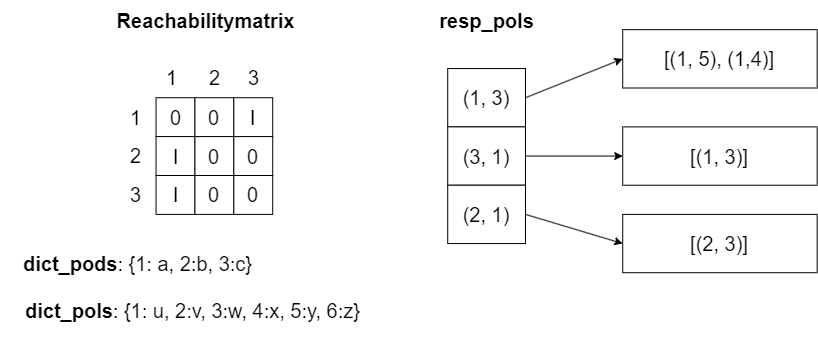
\includegraphics[width=0.8\textwidth]{images/store.png}
  \caption{Example of a reachabilitymatrix and some corresponding variables}
  \label{fig:store}
\end{figure}


% ==============================================
\section{Watcher} \label{impl:watcher} Execution of the algorithm starts by calling the main method of the watcher, which will then initialise all the other required components. The following flags and arguments are available when calling the watcher file:
\begin{itemize}
    \renewcommand{\labelitemi}{\scriptsize$\blacksquare$}
    \item \textbf{namespace:} The namespace in which the algorithm will look for conflicts (\textbf{required}).
    \item \textbf{verbose:} if the verbose flag is set, either by using -v or --verbose, the updated reachability matrix and corresponding container ids will be printed after each event (\textbf{optional}). 
    \item \textbf{debug:} If the debug flag is set, either by using -d or --debug, all data structures will be printed out to provide more information about changes in stored cluster state (\textbf{optional}).
    \item \textbf{startup:} If the debug flag is set, either by using -s or --startup, then a conflict detection will be executed when the algorithm is executed. This offers a quick conflict check of the current cluster state upon startup (\textbf{optional}).
\end{itemize}
When executed the watcher will start by collecting all the currently existing containers and network policies on the cluster in the namespace that is defined in the arguments. To do this it will leverage the Python Kubernetes library to retrieve lists of pods and policies, and pass them to the Parser to be turned into usable objects. These objects are passed to the analyzer which in turn calls upon the \acrlong{kic} to generate the base reachabilitymatrix using Kano's generative method. The analyzer also calls upon the \acrlong{sgic} to generate random security groups and security group rules and assign them to nodes. More information about the Analyzer, \acrshort{kic} and \acrshort{sgic} can be found in \autoref{impl:analyzer}, \autoref{impl:Kic} and \autoref{impl:sgic} respectively
\\[10pt]

After this initialisation stage the watcher is responsible for capturing all events on the cluster from Kubernetes by once again leveraging the Python Kubernetes library. It filters the resulting stream of data to find the six events defined in \autoref{tab:events} and adds them to an event queue to be handled. Container and policy events are outputted by different API endpoints of the Kubernetes cluster, so in order to watch these API's simultaneously multiple concurrent threads are required. To retrieve the events from the event queue and analyze them for changes in the cluster, all while maintaining the simultaneous monitoring of the API's, a third thread is introduced which we call the consumer. This thread will continuously take an event from the queue, send it to the analyzer for further handling, and await a response before going to the next event. This way the events are handled in the same order as their occurrence in the API's and only one event at a time. This prevents mistakes such as trying to analyze the deletion of a pod without it being present in the last saved cluster state, since the creation of that pod has not been handled yet. 
\\[10pt]
% ==============================================
\section{Analyzer} \label{impl:analyzer} The main task of the analyser is to handle all events received from the watcher. In order to do this it is closely coupled with the parser, \acrlong{kic} and \acrlong{sgic}, all of which are initialized during the analyzer's initialization. The $analyseEvent(event)$ function is the main reason of existence for the Analyzer and is shown in a simplified version in \autoref{algo:analyzer}. We will now briefly describe how it works.
\\[10pt]
the raw event data is first parsed into a policy or container object in the parser. It then immediately continues with calling the \acrshort{kic} to update the reachabilitymatrix with the new object. Although it is shown here as a single function call for any of the six events, it is actually different functions for each one which will be described in more detail in \autoref{impl:Kic}. The rest of the function's behaviour is dependant of the event type as well.
\\[10pt]
If the handled event is for a policy object then the size of the new reachability matrix has not changed: the amount of containers stays the same. We can thus create a deltamatrix by using the bitwise AND operation on the new reachabilitymatrix and the reachability matrix stored in the \acrshort{kic} that represents the previous cluster state. The result is a matrix of the same size as these reachability matrices but with a 1 on any position with a changed value and thus a changed container connection. By looking for these 1's in the deltamatrix we know where changes occur on which we can report and for which containers we must call upon the \acrshort{sgic} for conflict detection.
\\[10pt]
If a container event is being handled the size of the new reachability matrix will change due to the direct correlation between matrix size and the amount of containers in the cluster. The exception would be the container update event, which will use the deltamatrix in a similar fashion as the policy events in the previous paragraph. When handling a container delete or create event we start by looking at the matrix\_id of the object: If the container haS the matrix\_id $i$ then we look at position $[i][j]$ and $[j][i]$ in the matrix with $j\ in\ range(number\ of\ containers)$. We must be careful whether we use the new or previous-state reachability matrix for this position lookup: a delete event will mean the object is not present in the new reachabilitymatrix and vice-versa for the creation event. Afterwards we report on all these matrix positions where the value is 1: either a connection is made (create event) or a connection existed and is now removed (delete event). Lastly we call upon the \acrshort{sgic} conflict detection, which is described in \autoref{impl:sgic}.

\begin{algorithm}
    \caption{Event Analysis}
    \label{algo:analyzer}
    \begin{algorithmic}[1]
    \Function{analyseEvent}{event}
        \State obj $\gets$ parser.create\_object\_from\_event(event)
        \State new\_reach $\gets$ kic.update\_kano\_matrix(obj)
        \If{obj is a policy}
            \State deltamatrix $\gets$ kic.kano\_reach AND new\_reach
            \If{deltamatrix not all zeroes}
                \For{i, j where deltamatrix[i][j] == 1}
                    \State report changes
                    \State sgic.check\_sg\_connectivity(i.node, j.node, connection\_wanted)
                \EndFor
            \EndIf
            \\
        \ElsIf{obj is a container}
            \If{event['custom'] == "create"}
                \For{i in new\_reach.containers}
                    \If{new\_reach[obj][i] == 1}
                        \State report changes
                        \State sgic.check\_sg\_connectivity(obj.node, i.node, True)
                    \EndIf
                    \If{new\_reach[i][obj] == 1}
                        \State report changes
                        \State sgic.check\_sg\_connectivity(i.node, obj.node, True)
                    \EndIf
                \EndFor
            \ElsIf{event['custom'] == "delete"}
                \For{i in kic.containers}
                    \If{kic.kano\_reach[obj][i] == 1}
                        \State report changes
                        \State sgic.check\_sg\_connectivity(obj.node, i.node, False)
                    \EndIf
                    \If{kic.kano\_reach[i][obj] == 1}
                        \State report changes
                        \State sgic.check\_sg\_connectivity(i.node, obj.node, False)
                    \EndIf
                \EndFor
            \EndIf
        \EndIf
        \\
        \State update cluster state
    \EndFunction
  \end{algorithmic}
\end{algorithm}



% ==============================================
\section{Labeltree} \label{impl:labeltree}
Before continuing to the \acrlong{kic} we must briefly talk about the Labeltree. This custom data structure is used in the \acrshort{kic} to store all network policies of the current cluster state based on their selector labels (see section \ref{comp:label}). It is based directly on tree structures, with some changes in the update, delete and get methods to account for the key-value labels. \autoref{fig:labeltree} shows the structure of a labeltree: it always has a max depth of three, with depth one being the root node, depth two the keys of labels and depth three the values corresponding to the parent key. 
\\[10pt]

Because a network policy might have multiple selector labels the policy might be present in multiple leaf nodes. This is required so that, given a container with multiple labels, we can find all network policies that might apply to a single label. However, before assuming a policy applies to a container it must always be verified that all the selector labels of that policy are present in the container. The main reason to use this custom structure is it's constant date retrieval time due to the max tree depth of 3, and it's intuitive representation. 
\begin{figure}[htbp]
  \centering
  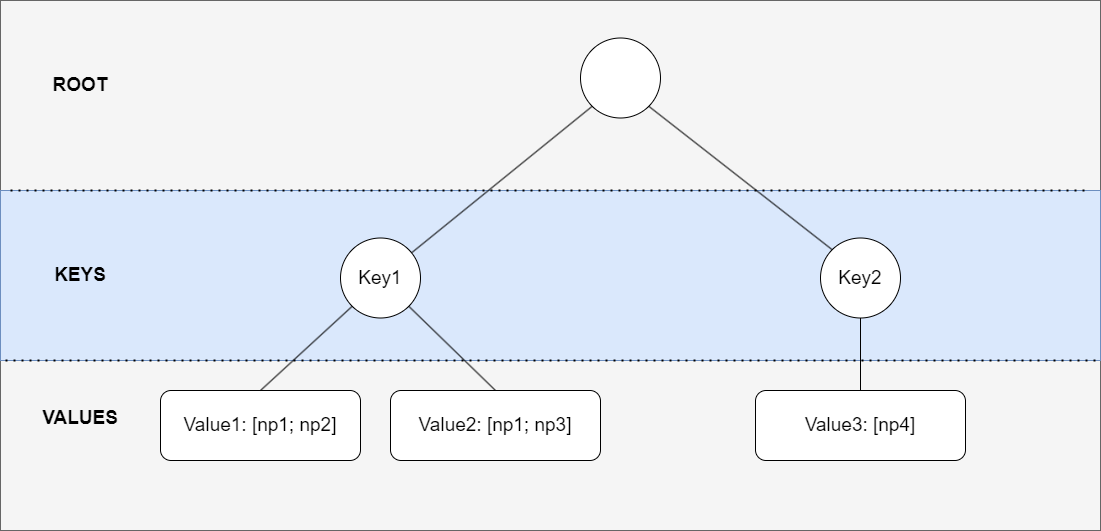
\includegraphics[width=0.8\textwidth]{images/labeltree.png}
  \caption{Structure of a Labeltree}
  \label{fig:labeltree}
\end{figure}

\newpage
% ==============================================
\section{Kubernetes Information Cluster} \label{impl:Kic}
The Kubernetes Information Cluster has two main functionalities: store all information about the current cluster state, and update the cluster state given an event. In order to achieve this first functionality the \acrshort{kic} stores the following variables:
\begin{itemize}
    \renewcommand{\labelitemi}{\scriptsize$\blacksquare$}
    \item \textit{egressTree:} The egress tree is a Labeltree used to store all the egress policies in the current cluster state.
    \item \textit{ingressTree:} The ingress tree is a Labeltree used to store all the ingress policies in the current cluster state.
    \item \textit{reachabilitymatrix:} This is a ReachabilityMatrix data structure that stores the current state in the format of a Kanomatrix and corresponding variables, as described in \autoref{impl:model}.
    \item \textit{pods:} A list of current containers
    \item \textit{pols:} A list of current network policies
\end{itemize}
Additionally the \acrshort{kic} also offers functions to update these variables. 
\\[10pt]
For the second functionality of updating the current cluster state and reachabilitymatrix when given an event different functions are required for different events. But before we can describe these functions we need to look at two smaller portions of the algorithm that reoccur often: getting all the containers that match all the label selectors in the allow set and similarly for the select set.
\\[10pt]

Both these algorithms use the same principle: for each label in a set of label selectors we retrieve the bitarray of containers that have this label applied according to the label\_map (see \autoref{kano:prefiltration}). We then do a bitwise AND operation to find the containers that have all these labels. When looking for the containers of the allow section of a network policy we must take into account that multiple label selector sets can exist. Therefore we retrieve the containers for each set separately and use a bitwise OR operation to find the final containers. This is described in \autoref{algo:select} and \autoref{algo:allow}. 
\\[10pt]
\begin{algorithm}
    \caption{Find containers matching the select labelselectors of a given policy}
    \label{algo:select}
    \begin{algorithmic}[1]
    \State \textbf{Input:} a network policy
    \State \textbf{Output:} bitarray of containers matching the select labelselector
    \State 
    \State  select\_containers\_final $\gets$ bitarray(0 * amount of containers)
    \State first $\gets$ True

    \For{select\_label in policy.selector}
        \State containers $\gets$ new\_reach.label\_map.get(select\_label)
        \If{containers is not empty}
            \If{first}
                \State first $\gets$ False
                \State select\_containers $\gets$ containers
            \Else
                \State select\_containers AND containers
            \EndIf
        \Else:
            \State select\_containers $\gets$ bitarray(0 * amount of containers)
            \State break
        \EndIf
    \EndFor

  \end{algorithmic}
\end{algorithm}
\begin{algorithm} 
    \caption{Find containers matching the allow labelselectors of a given policy} 
    \label{algo:allow}
    \begin{algorithmic}[1]  
    \State \textbf{Input:} a network policy
    \State \textbf{Output:} bitarray of containers matching the allow labelselector
    \State 
    \State  allow\_containers\_final $\gets$ bitarray(0 * amount of containers)
    \For{allow in policy.allow}
        \State allow\_containers $\gets$ bitarray(0 * amount of containers)
        \State first $\gets$ True
        
        \For{allow\_label in allow}
           \State containers $\gets$ new\_reach.label\_map.get(allow\_label)
           \If{containers is not empty}
                \If{first}
                    \State first $\gets$ False
                    \State allow\_containers $\gets$ containers
                \Else
                    \State allow\_containers AND containers
                \EndIf
            \Else:
                \State allow\_containers $\gets$ bitarray(0 * amount of containers)
                \State break
            \EndIf
        \EndFor
        \State allow\_containers\_final OR allow\_containers
    \EndFor
  \end{algorithmic}
\end{algorithm}

\newpage
For the final part of this subsection we will describe the functions in the \acrshort{kic} that are responsible for handling the events described in \autoref{tab:events} except the update events. Since each update has differences regarding the values that changed within the object the function handling these events would have to take into account many variables. Simply calling the delete and create method shortly after one another will get the same result instead. The functions that we created for the other four events all take an object as parameter which is either a container or policy object as seen in \autoref{impl:model}. We will now briefly describe each function and show their implementation in pseudo-code.  
\\[10pt]
\begin{itemize}
    \item \textbf{Delete Network Policy (\autoref{algo:deletepolicy}):} To delete a network policy we first copy the existing reachabilitymatrix to the new reachabilitymatrix. We then use \autoref{algo:select} and \autoref{algo:allow} to get bit arrays of all the containers that respectively match the select and allow label selectors. We use the labels of each container in the allow\_containers bitarray to find policies in the opposite direction with matching selector labels (i.e. if the deleted policy is ingress we look for an egress policy). In the following step we only need to check if these opposite policies match the select\_containers of the deleted policy with their allow label selectors. If this is the case we have a match and need to remove the responsible policies for these 2 containers, as well as update the matrix to include a 0 at the correct position if no other responsible policies between these containers exists.
    
    \item \textbf{add Network Policy (\autoref{algo:addpolicy}):} To add a network policy we follow the same steps as in the delete policy algorithm: we find the select container, the allow containers and the opposite policies, and if they all match up we got a match. However we now add a 1 to the correct position in the reachabilitymatrix and add to the resp\_policies instead of removing from it.
    
    \item \textbf{Delete Container (\autoref{algo:deletecontainer}):} To delete a container we first create a new reachabilitymatrix with one less row and column than the existing current state reachabilitymatrix. We then iterate over all the existing containers, get their corresponding row in the existing reachabilitymatrix, and remove the bit that corresponds to the deleted container before adding the edited row to the new reachabilitymatrix. We update the matrix\_ids by decrementing each one that is higher than the removed container's matrix\_id . Updating the label\_map of the containers is done similarly as to how the matrix has been updated: going over each bit array, removing the bit corresponding to the removed container and moving each bit behind the removed bit up by 1 position. Lastly the empty bit arrays get removed from the label\_map to remove unused labels.
    
    \item \textbf{Add Container (\autoref{algo:addcontainer}):} To add a container we first copy the existing reachabilitymatrix into the new\_reach variable and give a new matrix\_id to the container. By assigning a matrix\_id higher than that of all other containers we can guarantee that the new container is added at the end of the matrix for better visualization. Next we add a 0 on the end of each existing bit array and append a row of zeroes to the end of the reachabilitymatrix. following this we find all rules that are applied to this new container and store them in the rules set which will be traversed to find the containers that match the allow selectors of these rules using \autoref{algo:allow}. Now that we have a container that is selected by a policy that selects our new container, we must only find another network policy in the opposite direction. If such a \acrshort{np} exists a 1 is added  on the correct position of the reachabilitymatrix and all the related variables are updated.
    
\end{itemize}

\begin{algorithm}
    \caption{Delete policy from reachability matrix}
    \label{algo:deletepolicy}
    \begin{algorithmic}[1]
        \Function{reachabilitydeleteNP}{policy}
            \State new\_reachability $\gets$ kic.reachabilitymatrix
            \State select\_containers $\gets$ \autoref{algo:select}
            \State allow\_containers $\gets$ \autoref{algo:allow} 
            \State opposite\_policies $\gets$ \{\}
            \For{allow\_container in allow\_containers where bit == 1}
                \For{label in allow\_container.labels}
                    \If{policy is ingress}
                        \State treenode = egressTree.find(label)
                    \Else
                        \State treenode = ingressTree.find(label)
                    \EndIf
                    \For{policy2 in treenode}
                        \If{all labels in policy2.selector are in allow\_container.labels}
                            \State  opposite\_policies.add((policy2, allow\_container))
                        \EndIf
                    \EndFor
                \EndFor
            \EndFor
            
            \For{(policy2, allow\_container) in opposite\_policies}
                \For{select\_container in select\_containers where bit == 1}
                    \For{allow in policy2.allow}
                        \If{all labels from allow in select\_container.labels}
                            \State remove policy and policy2 from resp\_policies for the containers
                            \If{no responsible policies between the containers exist}
                                \State set bit in reachabilitymatrix to 0
                            \EndIf
                        \EndIf
                    \EndFor
                \EndFor
            \EndFor
            \State update variables
            \State \textbf{return} (new\_reachability)
        \EndFunction
  \end{algorithmic}
\end{algorithm}

\begin{algorithm}
    \caption{add policy to reachability matrix}
    \label{algo:addpolicy}
    \begin{algorithmic}[1]
        \Function{reachabilityaddNP}{policy}
            \State new\_reachability $\gets$ kic.reachabilitymatrix
            \State select\_containers $\gets$ \autoref{algo:select}
            \State allow\_containers $\gets$ \autoref{algo:allow} 
            \State opposite\_policies $\gets$ \{\}
            \For{allow\_container in allow\_containers where bit == 1}
                \For{label in allow\_container.labels}
                    \If{policy is ingress}
                        \State treenode = egressTree.find(label)
                    \Else
                        \State treenode = ingressTree.find(label)
                    \EndIf
                    \For{policy2 in treenode}
                        \If{all labels in policy2.selector are in allow\_container.labels}
                            \State  opposite\_policies.add((policy2, allow\_container))
                        \EndIf
                    \EndFor
                \EndFor
            \EndFor
            
            \For{(policy2, allow\_container) in opposite\_policies}
                \For{select\_container in select\_containers where bit == 1}
                    \For{allow in policy2.allow}
                        \If{all labels from allow in select\_container.labels}
                            \State add policy and policy2 to resp\_policies for the containers
                            \State set bit in reachabilitymatrix to 1
                        \EndIf
                    \EndFor
                \EndFor
            \EndFor
            \State update variables
            \State \textbf{return} (new\_reachability)
        \EndFunction
  \end{algorithmic}
\end{algorithm}

\begin{algorithm}
    \caption{Delete container from reachability matrix}
    \label{algo:deletecontainer}
    \begin{algorithmic}[1]
        \Function{reachabilityDeleteContainer}{container}
            \State new\_reachability $\gets$ $nXn$ matrix of bitarrays of 0's, with  n = \# of containers
            \State \Comment{Updating the reachability matrix}
            \For{i, cont in enumerate(containers)}
                \State row $\gets$ reachabilitymatrix[cont.matrix\_id]
                \State row.pop(cont.matrix\_id) \Comment{bit for the removed container}
                
                \If{container.matrix\_id \texttt{>} container.id}
                    \State container.matrix\_id -= 1
                \EndIf
                \State store row in new\_reachability
            \EndFor
            
            \State \Comment{Updating the label\_map matrix}
            \State new\_label\_map $\gets$ \{\}
            \For{label, old\_arr in reachabilitymatrix.label\_map.items()}
                \For{k in range(len(old\_arr))}
                    \If{k \texttt{>} container.matrix\_id}
                       \State new\_label\_map[label][k - 1] $\gets$ old\_arr[k] 
                    \ElsIf{k \texttt{<} container.matrix\_id}
                        \State new\_label\_map[label][k] $\gets$ old\_arr[k] 
                    \EndIf
                \EndFor
            \EndFor

            \State \Comment{Removing empty bitarrays from label\_map}
            \State new\_label\_map\_v2 $\gets$ \{\}
            \For{label, arr in new\_label\_map.items()}
                \If{\textbf{not} any bits set in arr}
                    \State delete new\_label\_map\_v2[label]
                \EndIf
            \EndFor
        
            \State new\_reachability.label\_map $\gets$ new\_label\_map\_v2
        
            \For{pod in pods}
                \If{pod.matrix\_id \texttt{>} container.matrix\_id}
                    \State pod.matrix\_id -= 1
                \EndIf
            \EndFor
        
            \State \textbf{return} (new\_reachability)
        \EndFunction
  \end{algorithmic}
\end{algorithm}

\begin{algorithm}
    \caption{Add container to reachability matrix}
    \label{algo:addcontainer}
    \begin{algorithmic}[1]
    \Function{reachabilityAddContainer}{container}
        \State new\_reach $\gets$ kic.reachabilitymatrix
        \State container.matrix\_id $\gets$ len(containers)
        \State matrixId\_to\_Container[container.matrix\_id] = container
        \For{label, array in label\_map}
            \State array.append(False)
        \EndFor
        \For{row in new\_reach} 
            \State row.append(0)
        \EndFor
        \State new\_reach.append(bitarray(0 * amount of containers))
        \State rules = Set()
        \For{label in container.labels}: 
            \For{policy in eggressTrie.find(label)}
                \If{all policy.select.label in container.labels}
                    \State rules.add
                \EndIf
            \EndFor
            \For{policy in ingressTrie.find(label)}
                \If{all policy.select.label in container.labels}
                    \State rules.add
                \EndIf
            \EndFor
        \EndFor
        \For{rule in rules}
            \State allow\_containers $\gets$ \autoref{algo:allow} 
            \For{secondcontainer in allow\_containers}
                secondRules = Set()
                \For{secondlabel in secondcontainer.labels}:
                    \For{policy in eggressTrie.find(label)}
                        \If{all policy.select.label in container.labels}
                            \State secondRules.add
                        \EndIf
                    \EndFor
                    \For{policy in ingressTrie.find(label)}
                        \If{all policy.select.label in container.labels}
                            \State secondRules.add
                        \EndIf
                    \EndFor
                \EndFor
                \For{secondrule in secondRules}
                    \If{all labels of secondrule.selector in secondcontainer}
                        \For{secondallow in secondrule.allow}
                            \If{all labels of secondallow in container.labels}
                                \State update the matrix for new connection
                            \EndIf
                        \EndFor
                    \EndIf
                \EndFor    
            \EndFor 
        \EndFor   
        \State \textbf{return} new\_reachability
    \EndFunction
  \end{algorithmic}
\end{algorithm}



% ==============================================
\newpage
\section{Security Group Information Cluster} \label{impl:sgic}
Since handling cloud layer events is out of scope for this thesis we also have no need to actively monitor the cloud layer. Therefore the \acrlong{sgic} mimics the security groups and security group rules one might find in the cloud layer by generating them with randomised variables when the Watcher is initialized. Security group objects are based upon the Openstack Security Group definitions, which means they contain a list of rules and have a unique name \cite{secgroups}. The amount of rules in each security group is randomised as well, and each rule contains variables such as port, direction, protocol and ethertype filled with randomised values. Additionally a security group rule targets other nodes by either a single remote IP, an IP with a subnetmask to act as a range of IPs, or the name of another existing security group which targets all nodes part of that security group.
\\[10pt]

Once the security groups and their rules are created each node in the Kubernetes cluster gets linked to one or multiple security groups. We then use directed graphs to store allowed connections, where nodes are the vertices and an edge between two nodes indicates that connection is allowed in that direction. Each edge includes the security group and \acrshort{sg} rule number responsible for the connection. Thereafter both an ingress and egress graph get created and filled by going trough all security groups, finding their nodes and adding the corresponding security group rules to these nodes in the graphs. We then use these 2 directed graphs to create a VMmatrix of size \(kxk\) where \(k\ =\ amount\  of\  nodes\  in\  the\  cluster\), similarly to the Kano reachabilitymatrix. When an edge is present in both graphs the connection is allowed in both directions and thus results in a 1 in the VMmatrix. Since we created the directed graphs we can easily retrieve responsible security groups and \acrshort{sg} rules for a specific node connection. The VMmatrix on the other hand quickly tells us whether or not the connection is possible in the first place.
\\[10pt]

The \acrlong{sgic} is also responsible for conflict detection between the cloud and cluster layer. Once the \acrshort{kic} finishes creating the updated reachabilitymatrix the Analyzer will call the check\_sg\_connectivity function in the \acrshort{sgic} which we will now explain with the help of \autoref{algo:connectivity}. The function takes three parameters: 2 node names and a boolean indicating whether or not a connection between these 2 nodes is wanted. E.g. a newly created container can communicate to another container on a different node: then the function gets called with the boolean connection\_wanted set to True. The function will then print out whether or not the nodes are able to communicate by looking at the VMmatrix and print out the responsible security groups and security group rules by retrieving them from the directed graphs. If the connection is contradictory to the boolean we report a conflict.

\begin{algorithm}
    \caption{Conflict detection}
    \label{algo:connectivity}
    \begin{algorithmic}[1]
    \Function{check\_sg\_connectivity}{node1, node2, connection\_wanted}
        \State print security groups for node1
        \State print security groups for node2
        \If{vmMatrix[node1, node2] == 1}
            \If{connection\_wanted == True}
                \State print security group rules responsible for connection 
            \Else
                \State report conflict with responsible security group rules
            \EndIf
        \EndIf
        \If{vmMatrix[node2, node1] == 1}
            \If{connection\_wanted == True}
                \State print security group rules responsible for connection 
            \Else
                \State report conflict with responsible security group rules
            \EndIf
        \EndIf
    \EndFunction
  \end{algorithmic}
\end{algorithm}





\cleardoublepage




\newpage
%!TeX root=../../main.tex
\chapter{Evaluation}                                 \label{ch:evaluation}
This chapter aims to evaluate our algorithm described in chapter 3. This evaluation will be based on 4 research questions, split up into 2 experiments. The first experiment will be a comparison between Kano and the comparable part of our algorithm that is responsible for incrementally updating the matrix. The second experiment is a general test of our overall algorithm in terms of time and memory consumption. Both of the evaluation experiments are run on the same cluster setup and share configuration specifics, which we will describe in the first section. The second and third sections will talk about the first and second experiment respectively and include subsections about the experiments' approach, setup and results. We end with an overview of  conclusions drawn from the experiments
\\[10pt]

% =========================================
\section{Evaluation setup} \label{sec:evalsetup}


The Kubernetes cluster used for the experiments consists of 8 nodes: 7 workers nodes and a single control-plane node that does not run any containers. Each of these nodes are located on its own \acrshort{vm}, which are deployed as instances on the Openstack installation of the Department of Computer Science at KULeuven. Each instance has 2 VCPUs, 4GB RAM and 20GB memory, and runs Ubuntu 22.04 jammy for its OS. There are no Security Groups applied to the instances except for the default. Calico is used as \acrshort{cni} to provide the connection between the Kubernetes nodes, which all run on the Kubernetes Git version v1.22.17. Kubernetes runs on default settings and specifies the maximum amount of pods per worker node at around 100 pods.
\\[10pt]

Each pod we deploy is created with the latest nginx image, which is version 1.25.3 at the time of the experiments and writing. \autoref{fig:podyaml} shows the pod manifest structure for each deployed pod, with $name$ and $labels$ randomly generated and $ns$ depending on the execution arguments which we will describe in the next sections. As shown in the picture the pods are specified to not use any resources when deployed. The experiment algorithms are executed on the control-plane node and will execute without the need for interaction, on the condition that the specified namespace used for the experiment already exists on the cluster.
\\[10pt]
\begin{figure}[htbp]
  \centering
  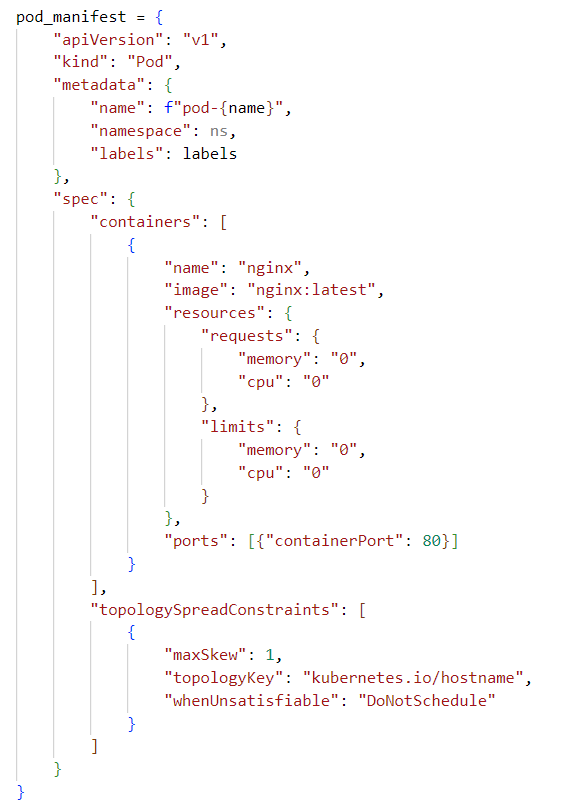
\includegraphics[width=0.6\textwidth]{images/podyaml.png} 
  \caption{Template for pod creation}
  \label{fig:podyaml}
\end{figure}

Each experiment will be run once for each of the events described in \autoref{tab:events} since they can differ in space and time cost. For example, removing a container might be faster than adding a new container, since the first mainly just removes data while the latter includes a search for matching network policies according to its labels. However, we only measure four out of the six events that we can capture, since updating network policies and containers equals directly to first executing a deletion event, directly followed by a creation event. The update events can thus be calculated from the creation and deletion events saving time when executing the experiments.
\\[10pt]

We want to know how each experiment behaves when the cluster size increases in terms of pods and network policies. For this reason, we define 5 cluster setups that define variables such as number of pods and number of network policies. The combinations of 5 cluster setups and 4 events gives us a total of 20 smaller experiments for each experiment,  which we will call sub-experiments.  Each of these 20 sub-experiments is run a hundred times giving us a total of 2000 runs and their respective data per experiment.
\\[10pt]


% =========================================
\section{Experiment 1}\label{sec:experiment1}
Kano is a research solution that verifies network policies based on the reachabilitymatrix it generates when provided with a list of pods and a list of policies. For some background about Kano, we refer to \autoref{sec:kano}. Kano only has a generative algorithm to create this reachabilitymatrix, while our solution provides an incremental approach that updates the reachabilitymatrix instead of regenerating it. Naturally, a comparison between each approach is required and will be described in this section. This comparison will be used to answer the following two research questions:

\begin{itemize}
    \item \textit{Q1:} What is the difference in time cost between an incremental update of the Kano matrix compared to newly generating the Kano matrix for every event and how does this difference scale with pod/policy numbers
    \item \textit{Q2:} What is the difference in space cost between an incremental update of the Kano matrix compared to newly generating the Kano matrix for every event and how does this difference scale with pod/policy numbers
\end{itemize}

Before we delve into the experiment approach, setup and results we declare our hypotheses for these questions:

\begin{itemize}
    \item \textit{Hypothesis Q1:} We predict that the time cost of our incremental approach will be higher in small clusters due to the writing times of variables, but will prove better than the time cost of the generative approach as the cluster increases since the incremental approach does not have to verify all network policies and containers.
    \item \textit{Hypothesis Q2:} We predict that the space cost of the incremental approach will be higher than that of the generative approach due to the memory required for storing the current cluster state. We predict this difference will only increase as the cluster increases in size.
\end{itemize}

% =========================================
\subsection{Approach} \label{exp1:approach}
Since our algorithm does much more than just updating the reachabilitymatrix we first have to remove the irrelevant parts from our codebase. The \acrlong{sgic} is removed from the algorithm altogether, while the Analyzer gets modified so that it only calls upon the \acrlong{kic} to update the reachabilitymatrix. As a result, the analyzer does not use the updated matrix to compare it with the previous cluster state nor does it print out any information anymore. This adapted algorithm for the incremental approach now allows for a direct comparison with Kano's generative approach.  For both approaches, we want to collect the time (ms), memory at the start of the method (MB), the highest memory peak during execution of the method (MB) and  the difference between the peak and start memory (MB)
\\[10pt]

Each event type will be tested in 5 different setups which will be identical for each event and are described in \autoref{tab:exp1pars}. These parameter values are based on the parameters used in the evaluation of Kano \cite{kano}. However, our maximum number of pods and policies is lower than Kano's evaluation due to the limits of our experiment cluster. We will now summarize the meaning of each parameter:
\begin{itemize}
    \item \textit{Pod num}: This variable describes the number of pods that will be generated and deployed on the cluster. Each pod has a single container thus this variable directly annotates the amount of containers as well.
    \item \textit{Pol num}: This variable describes the number of network policies that will be generated and deployed on the cluster.
    \item \textit{key limit}: This variable describes the number of distinct keys out of which one will randomly be selected each time a key-value label is generated. The lower this number, the higher the chance of matches between containers and network policy label selectors.
    \item \textit{Value limit}: This constant describes the number of distinct values out of which one will randomly be selected each time a key-value label is generated.
    \item \textit{Pol select limit}: This constant describes the amount of selector fields in a network policy.
    \item \textit{Pol select label limit}: This constant describes the maximum amount of label selectors in a selector field of a network policy. each selector field will thus have between 1 and this value's amount of randomised label selectors.
    \item \textit{Pol allow limit}: This constant describes the maximum amount of allowed fields in a network policy. each network policy will thus have between 1 and this value's amount of allowed fields.
    \item \textit{Pol allow label limit}: This constant describes the maximum amount of allow selectors in an allow field of a network policy. each allow field will thus have between 1 and this value's amount of randomised label selectors.
     \item \textit{Pod label limit}: This constant describes the maximum amount of labels in a container. Each container will thus have between 1 and this value's amount of randomised key-value labels.
\end{itemize}

\begin{table}[H]
    \centering
    \begin{tabular}{|l|c|c|c|c|c|}
        \hline
        \textbf{Name} & \textbf{setup 1} & \textbf{setup 2} & \textbf{setup 3} & \textbf{setup 4} & \textbf{setup 5}\\
        \hline
        Pod num & 50 & 100 & 250 & 500 & 750 \\
        Pol num & 20 & 50 & 100 & 200 & 300 \\
        Key limit & 2 & 5 & 8 & 10 & 20 \\
        Value limit & 10 & 10 & 10 & 10 & 10 \\
        Pol select limit & 1 & 1 & 1 & 1 & 1 \\
        Pol select label limit & 3 & 3 & 3 & 3 & 3 \\
        Pol allow limit & 3 & 3 & 3 & 3 & 3 \\
        Pol allow label limit & 3 & 3 & 3 & 3 & 3 \\
        Pod label limit & 5 & 5 & 5 & 5 & 5 \\
        \hline
    \end{tabular}
    \caption{Experiment 1 parameter values}
    \label{tab:exp1pars}
\end{table}

% =========================================
\subsection{Execution} \label{exp1:execution}
 We will now describe the execution of a single sub-experiment step by step.
\\[10pt]

\textbf{STEP 0:} Call the python file experiment1.py with the following arguments: $number\_of\_runs$, $number\_of\_pods$, $number\_of\_policies$, $namespace$, $key\_limit$ and $event\_type$ according to the sub-experiment settings. The algorithm will then execute STEP 1 to STEP 7 as many times as defined in argument $number\_of\_runs$.
\\[10pt]

\textbf{STEP 1:} We fully reset the namespace defined in the $namespace$ argument with the help of the Python Kubernetes API. This is coded in a separate delete.py file and extended with some extra tests and timeouts to guarantee that all objects are successfully removed before continuing.
\\[10pt]

\textbf{STEP 2:} We deploy as many pods and network policies as defined in arguments \newline $number\_of\_pods$ and $number\_of\_policies$. For this functionality a separate deploy.py python file has been created that will generate and deploy the network policies and pods, when called upon with the variables $namespace$ and $key\_limit$ as parameters. The other relevant constants in \autoref{tab:exp1pars} are hard coded since they don't change between sub-experiments. The deploy file is equipped with a list of distinct keys and values to leverage when creating the randomised pods and \acrshort{np}s. However, the key list is first shortened until it has a length equal to the $key\_limit$ parameter before being utilised. The randomised pods and network policies get deployed in the namespace defined in the $namespace$ argument with the help of the Python Kubernetes API. We use extra tests and timeouts to guarantee all objects are successfully deployed and ready before continuing.
\\[10pt]

\textbf{STEP 3:} We start the watcher with the flags for debug mode, verbose mode and start the checkup all set to False. With the use of threading events, we guarantee that the threads that watch the APIs for pods and \acrshort{np}s are successfully running, to prevent the next step from executing too early, therefore missing the event and being unable to handle it.
\\[10pt]

\textbf{STEP 4:} We execute one event, depending on the $event\_type$ argument. If it is a delete event we call the delete.py file again and let it randomly remove one of the existing objects that correspond to the event type. If it is a deploy event we call the deploy.py file to generate one more randomly generated object according to the correct parameters.
\\[10pt]

\textbf{STEP 5:} We once again leverage threading events to get notified when the consumer thread has received and handled its first event. Since the watcher was initialized after all pods and network policies were fully ready it will always be the event from step 4 that will be caught. When the consumer catches the event it will start the timer right before calling the analyzer for event handling. Once the analyzer returns the function call the timer immediately gets stopped to get a final execution time. Similarly, we measure the memory usage at the start of the algorithm, and the highest peak of memory usage during the event handling. With this we can calculate the difference and thus how much memory was used (in bytes). These memory and time measurements get stored in variables in the watcher.
\\[10pt]

\textbf{STEP 6:} Once we get the message that the event is handled we retrieve the measurements from the watcher and store it locally. We can then stop the watcher.
\\[10pt]

\textbf{STEP 7:} We now call retrieve all existing pods and \acrshort{np}s in the cluster and put them in lists.  Once we have started a new timer and started tracing memory we give these lists to the original matrix generation method from Kano. Upon return of the reachabilitymatrix, the timer and memory measurement are stopped and stored in variables. We also include a comparison between the incremental and generative reachabilitymatrices to ensure the results are correct and no bugs or edge cases were discovered. If the latter is the case the sub-experiment is cancelled and debug information is printed out.
\\[10pt]

\textbf{STEP 8:} Once the hundred runs of the sub-experiment have finished we store all the data in a CSV file and store it on the control plane node that ran the experiment. We can then retrieve this file and combine it with other sub-experiment files for evaluation. 
\\[10pt]


% =========================================
\subsection{Experiment results} \label{exp1:results}

The results of the experiment will be divided into eight different graphs: for each event type, we created a graph displaying average and median time as well as a graph that shows average and median memory consumption. All the graphs use the same values and increments on their axis to allow a direct comparison. We will start by looking at the time graphs after which continue with the memory results.
\\[10pt]

\textbf{Time consumption}
\newline When looking at the graphs in \autoref{fig:exp1-addNP-time}, \autoref{fig:exp1-addPod-time}, \autoref{fig:exp1-delNP-time}  and \autoref{fig:exp1-delPod-time} we can quickly deduce that our incremental approach starts more time expensive but becomes faster as the scale of the cluster increases. This trend seems to continue as the cluster grows and is in line with our hypothesis for Q1 described in \autoref{sec:experiment1}. We will now take a deeper look into the data and describe some additional observations:

\begin{itemize}
    \item If we look at the intersection point of the generative and incremental averages we see a difference between \acrshort{np} and pod events. For the network policy events, the intersection always appears between the third and fourth sub-experiment, while for the pod events, this is closer the the third sub-experiment. This can be explained due to the different approaches: when a \acrshort{np} is added or deleted all the pods with the corresponding labels must be retrieved, while a pod addition or deletion needs to find the corresponding network policies. Since our experiment settings always have more pods than network policies the search time for network policy events naturally becomes higher.
    
    \item Thanks to the included median values we see that the deletion events have fewer outlying values compared to the creation events. This can be explained once again by the approach to handle these events: when creating a pod or \acrshort{np} the time will be influenced by the number of matching label selectors between pods and network policies, which is randomised for each run. When deleting an object we do not need to search for a match between selectors, instead, we simply remove the information from the cluster state, thereby saving time.
    
    \item Although the generative approach from Kano stays consequent throughout the four events our solution is more dependent on the type of event being handled. The incremental approach stays in the similar range of values for the first sub-experiments, but as the cluster size increases the pod events generally take less time to update the reachabilitymatrix compared to the similar \acrshort{np} event. 
    
    \item Although update events for containers and \acrshort{np}s are not measured for reasons stated earlier in this chapter we can try to make some assumptions about them. Since the method for handling update events equals executing the deletion and then creation of the object in question, we can add these separate values together for an estimate. With the fifth sub-experiment setting the incremental approach already outperforms the generative for updating pods: the average time for adding a pod ($\sim$182 ms) combined with the average time for deleting a pod ($\sim$209 ms) is still lower than the time it takes for the generative approach ($\sim$466 ms). Additional testing in future work would be required to draw more conclusions about this, but it is reasonable to assume that the trend continues and that there will be a cluster size for which the incremental approach intersects with the generative approach for update events, after which the incremental approach outperforms the generative for larger cluster sizes.
\end{itemize}

\begin{figure}[H]
    \centering
    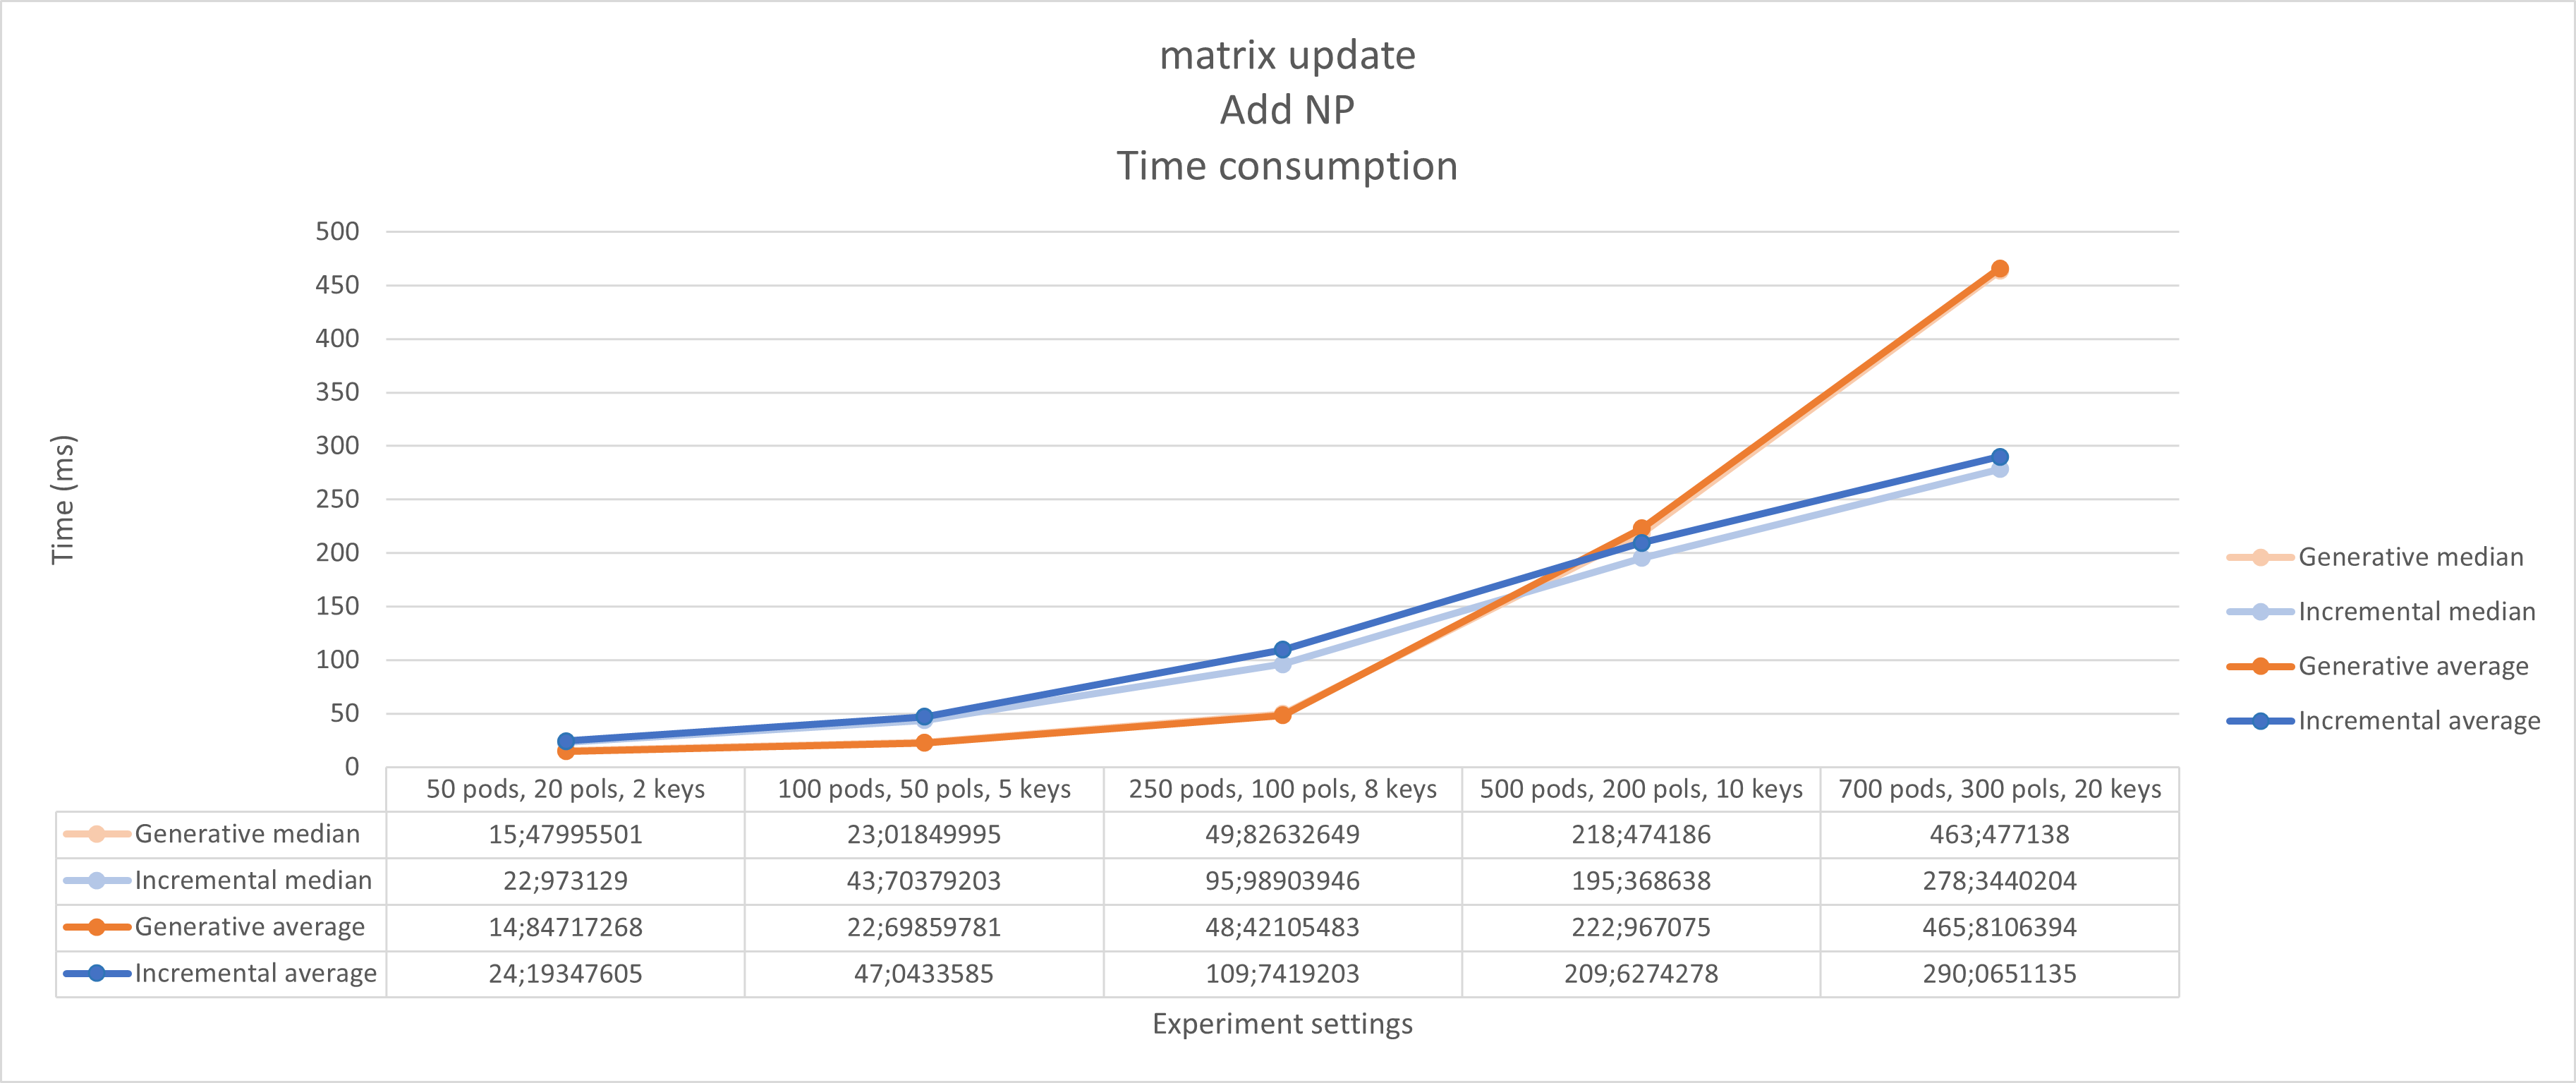
\includegraphics[width=\textwidth]{images/experiment1/addNP-time.png}
    \caption{Time consumption of adding a network policy}
    \label{fig:exp1-addNP-time}
\end{figure}
\begin{figure}[H]
    \centering
    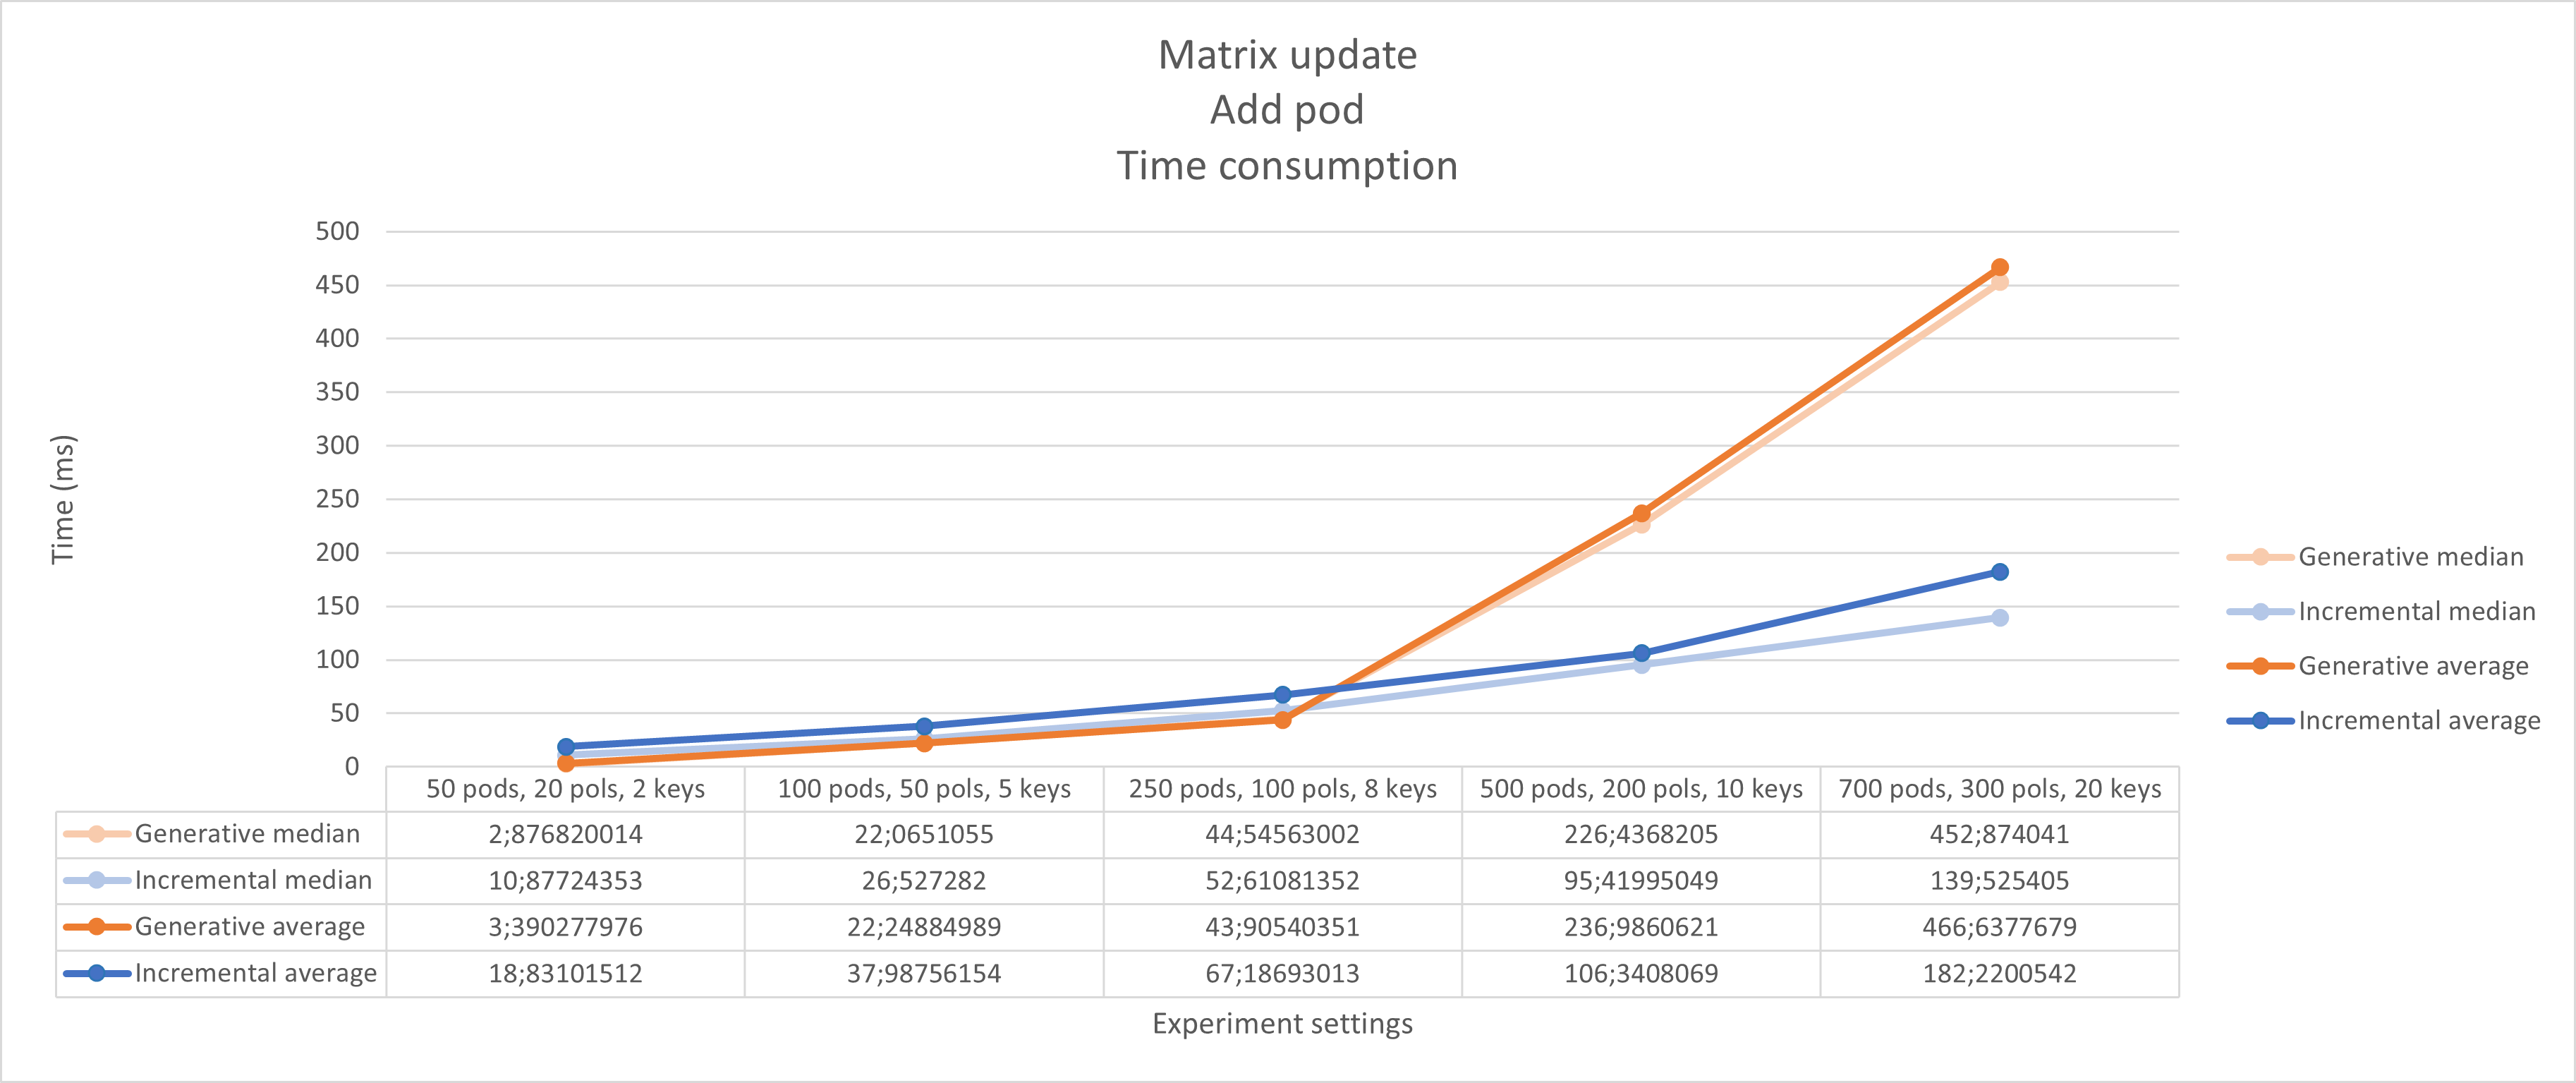
\includegraphics[width=\textwidth]{images/experiment1/addPod-time.png}
    \caption{Time consumption of adding a container}
    \label{fig:exp1-addPod-time}
\end{figure}
\begin{figure}[H]
    \centering
    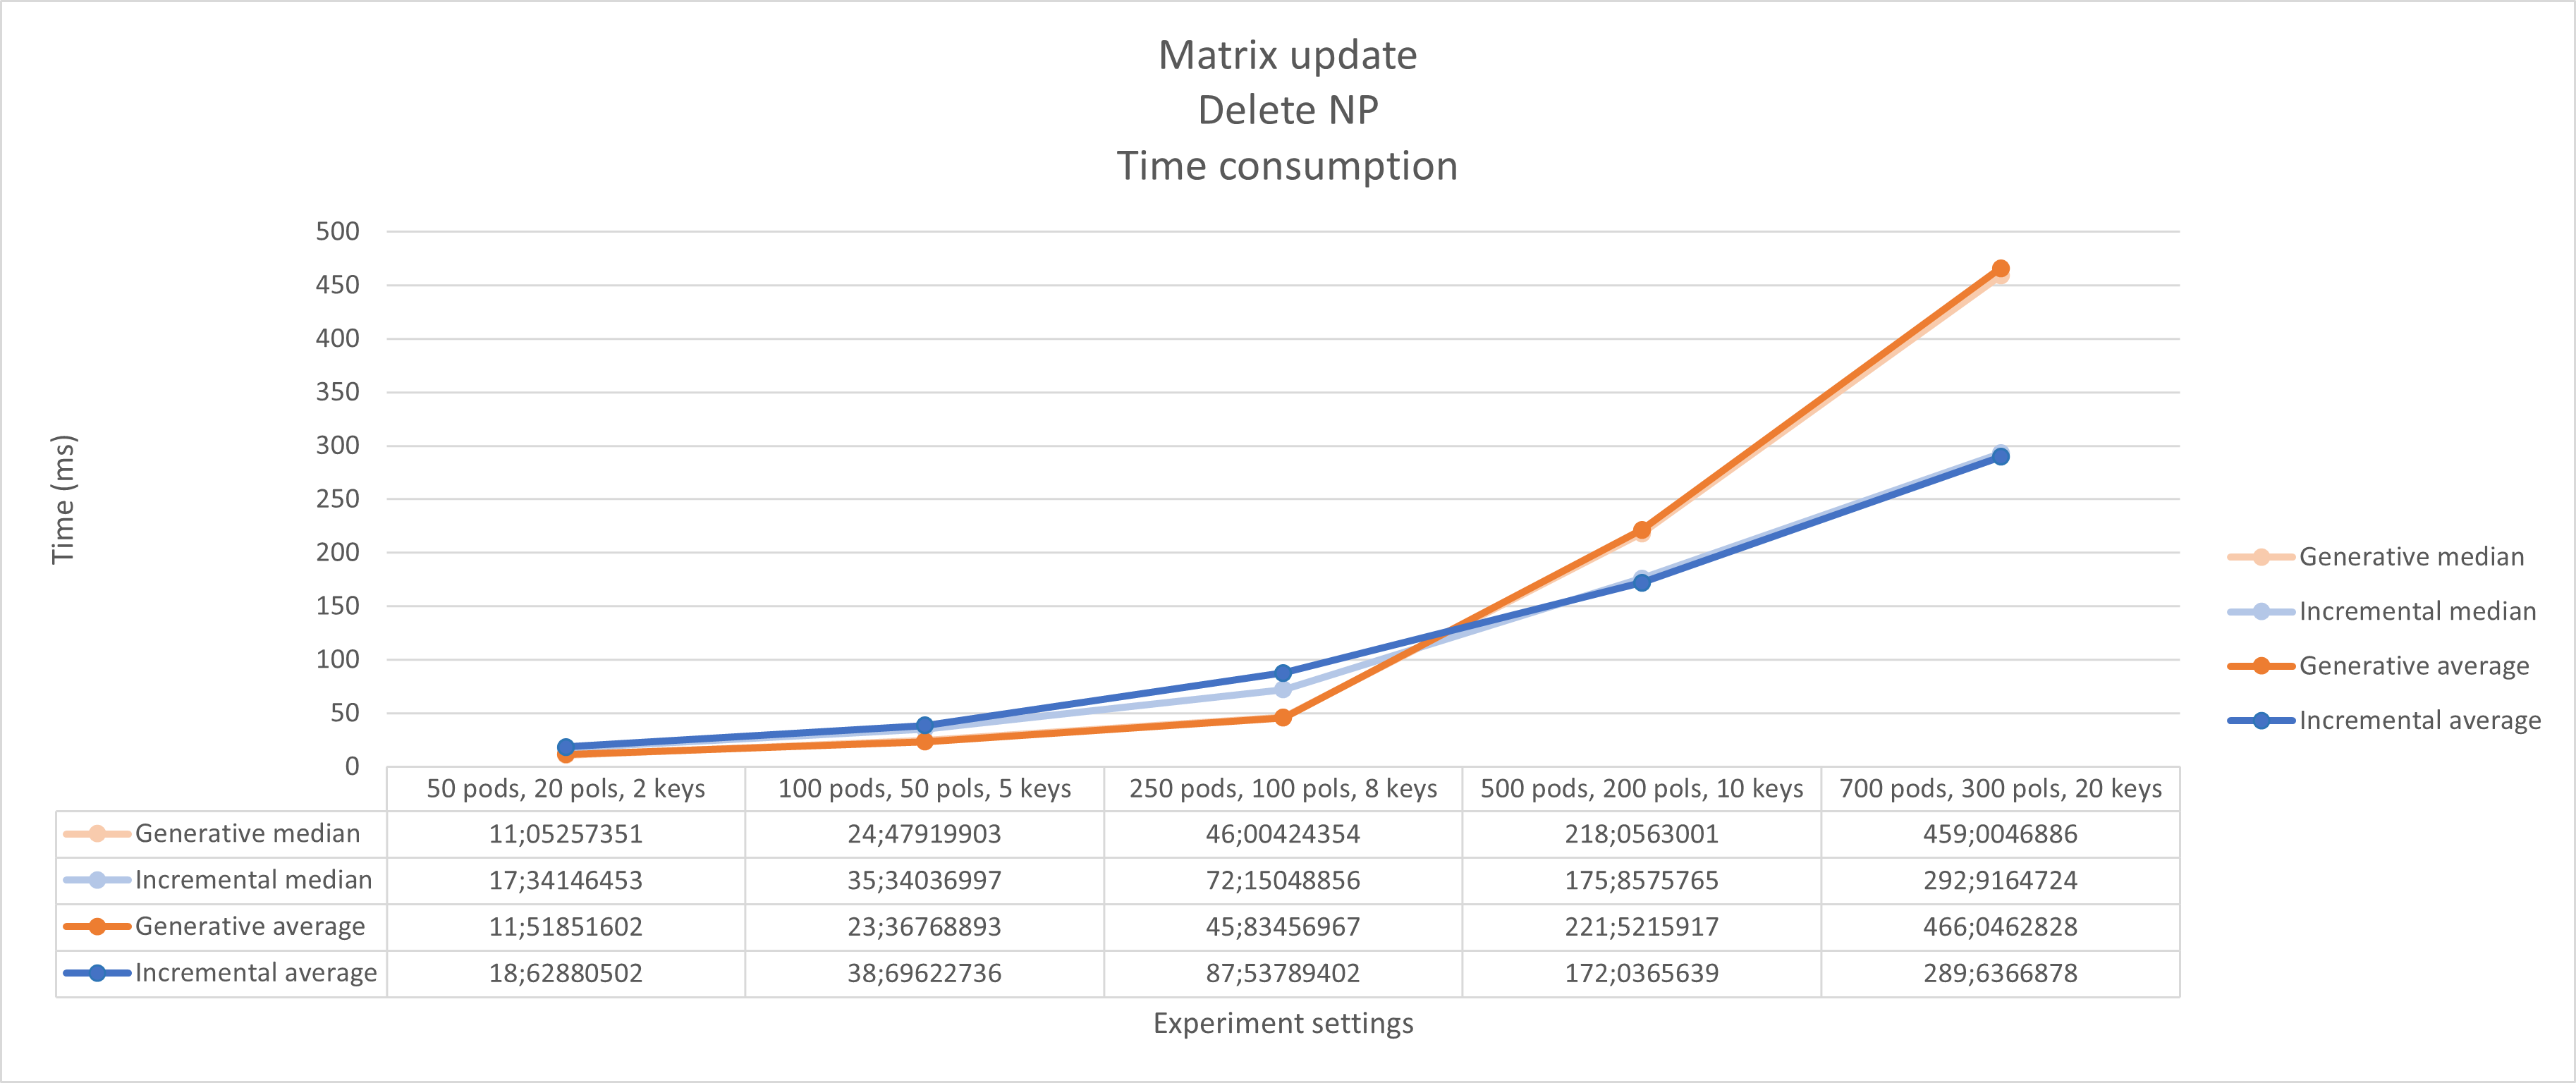
\includegraphics[width=\textwidth]{images/experiment1/delNP-time.png}
    \caption{Time consumption of deleting a network policy}
    \label{fig:exp1-delNP-time}
\end{figure}
\begin{figure}[H]
    \centering
    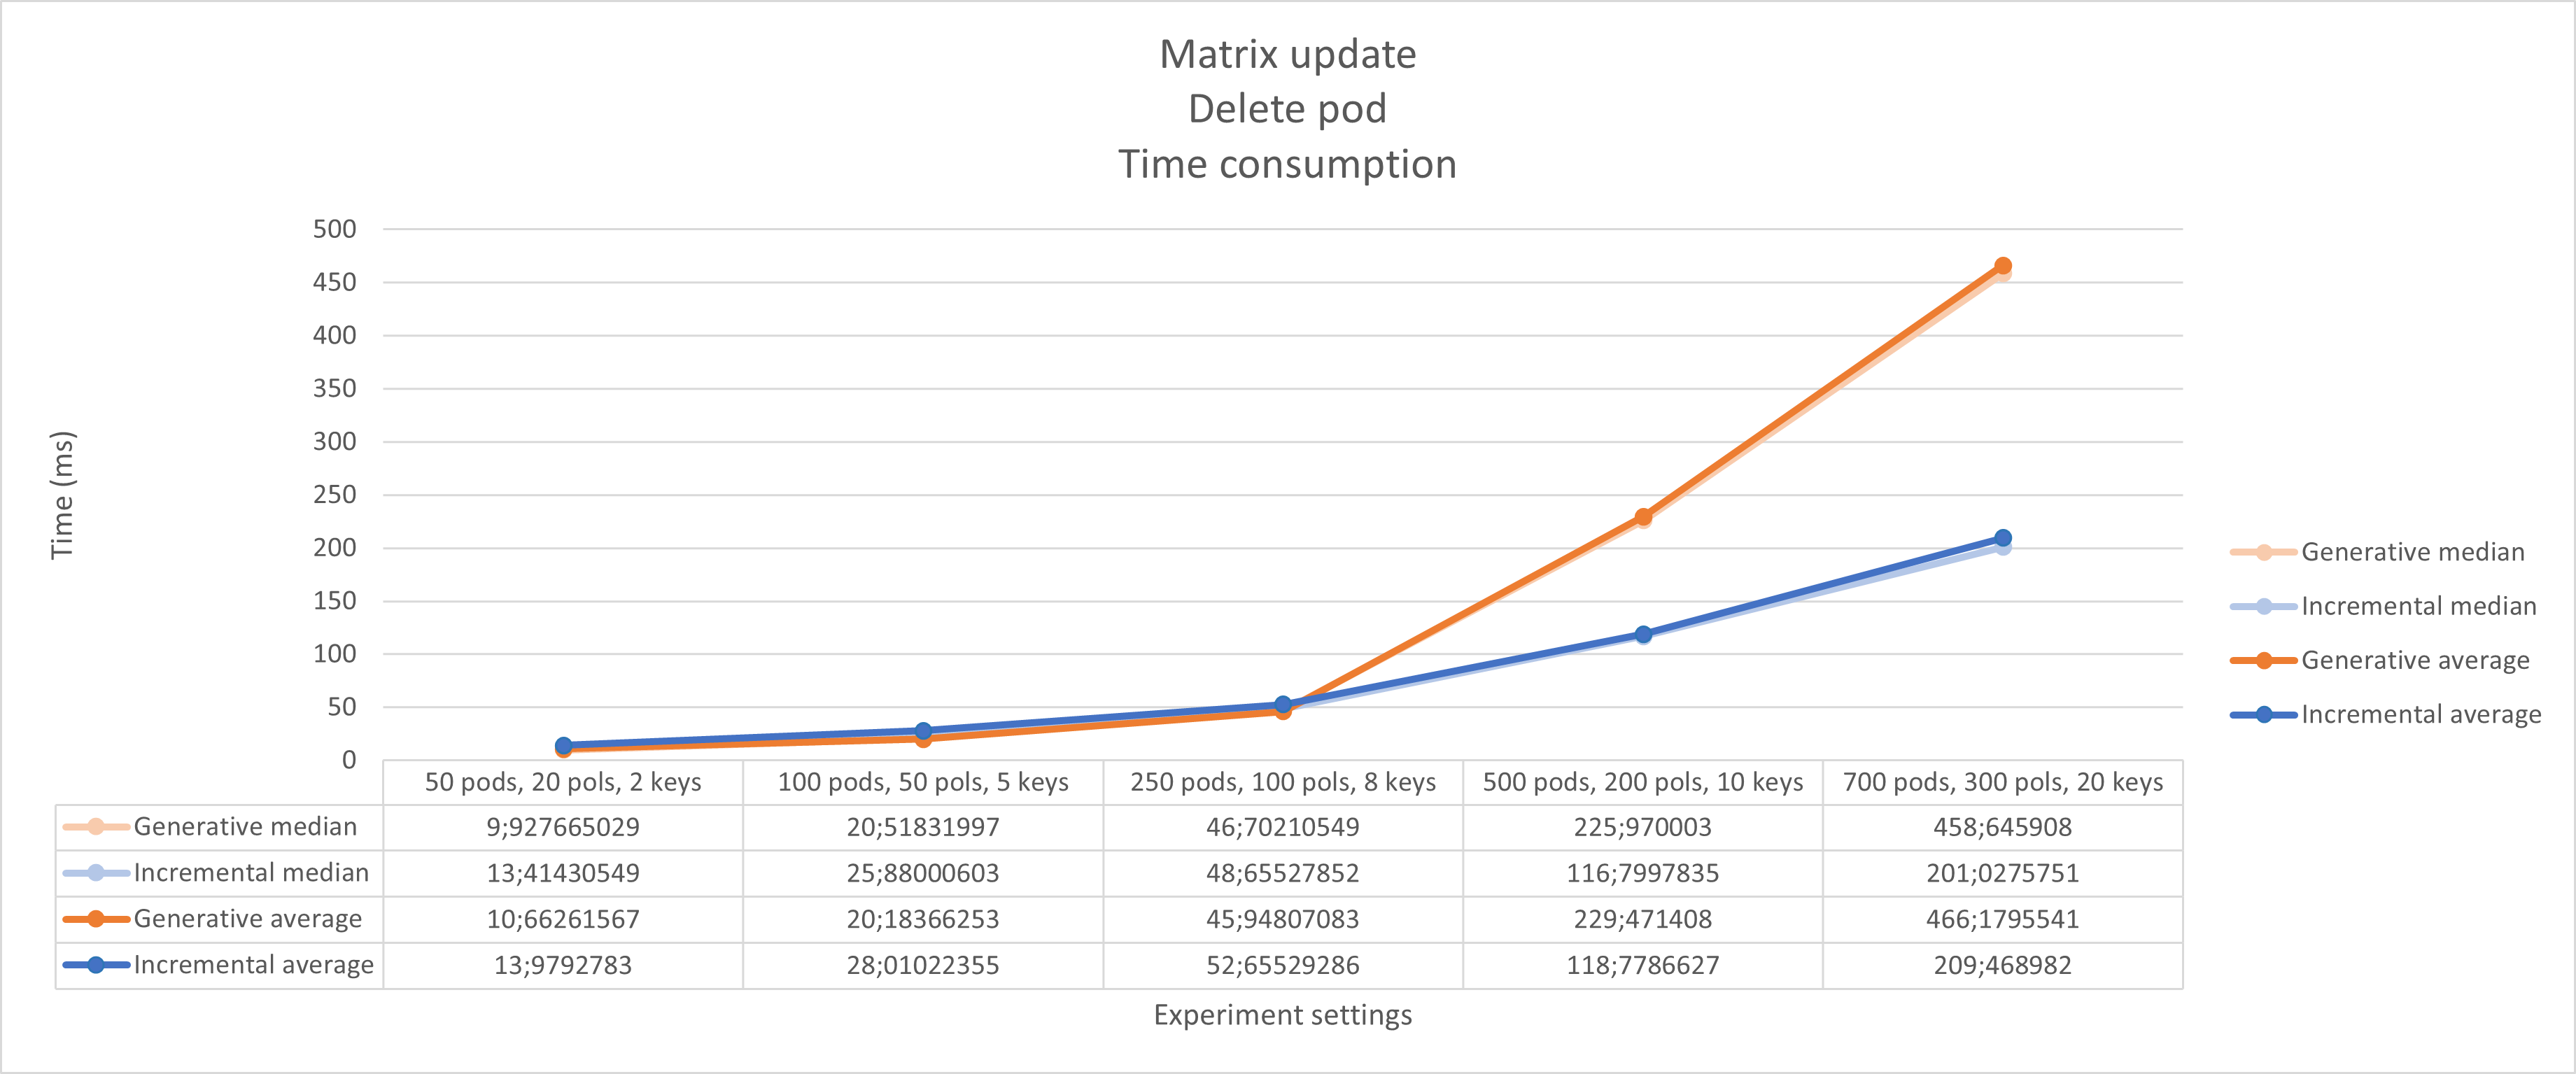
\includegraphics[width=\textwidth]{images/experiment1/delPod-time.png}
    \caption{Time consumption of deleting a container}
    \label{fig:exp1-delPod-time}
\end{figure}



\textbf{Memory consumption}
\newline When looking at the graphs in \autoref{fig:exp1-addNP-memory}, \autoref{fig:exp1-addPod-memory}, \autoref{fig:exp1-delNP-memory}  and \autoref{fig:exp1-delPod-memory} we can quickly deduce that our incremental approach is more expensive in terms of memory usage than the generative approach, with the difference only increasing as the cluster grows. This is in line with our hypothesis for Q2 described in \autoref{sec:experiment1}. Next, we present some additional observations we can deduce from these graphs:
\begin{itemize}
    \item With a small exception for the fifth sub-experiment in the creation event of a network policy, the median values are almost identical to the average values, meaning little skewing of data between the runs occurs. This makes sense since the cluster state that we store always has the same amount of cluster objects to keep track of within each run. The exception mentioned before might be due to a high occurrence of matching labels between objects which in turn increases the size of data structures such as the Store keeping track of \acrshort{np}s responsible for connections between pods. However, this remains an educated guess at best.
    \item We can see that the ratio in which the memory increases for the incremental method decreases slightly between the fourth and fifth sub-experiments. We have no direct explanation for this, and further research would be necessary to deduct more from this. 
 	\item Although the incremental approach has higher memory consumption it should be noted that the generative approach can not be used in its current form to execute conflict detection and would need adaptations to store more information. We can therefore not conclude that our incremental approach is strictly worse in terms of memory consumption than the generative approach.
\end{itemize}

\begin{figure}[H]
    \centering
    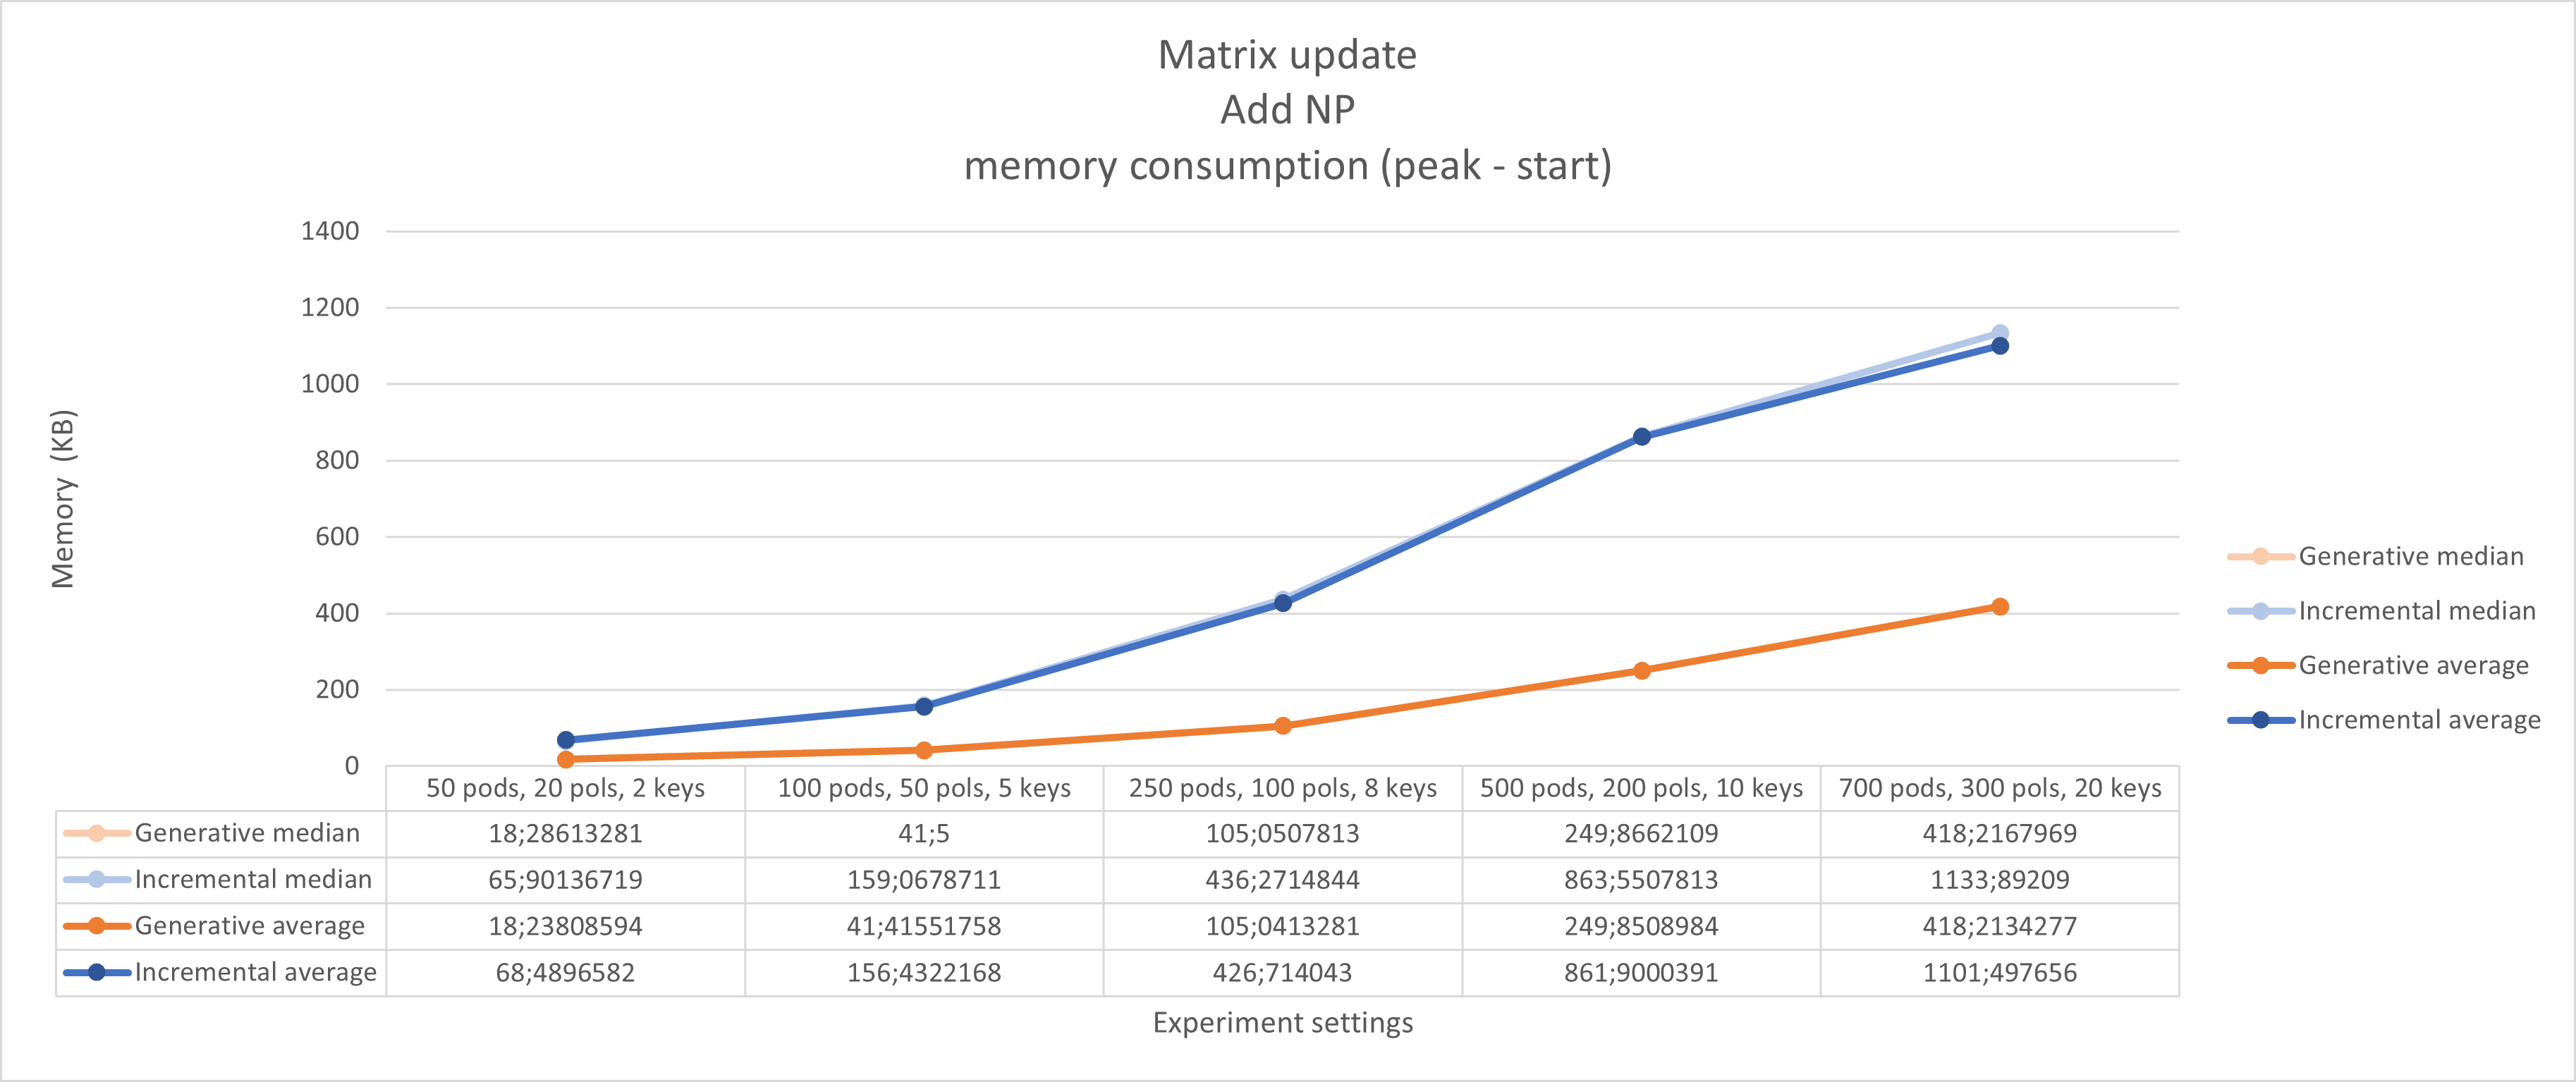
\includegraphics[width=\textwidth]{images/experiment1/addNP-memory.png}
    \caption{Memory consumption of adding a network policy}
    \label{fig:exp1-addNP-memory}
\end{figure}
\begin{figure}[H]
    \centering
    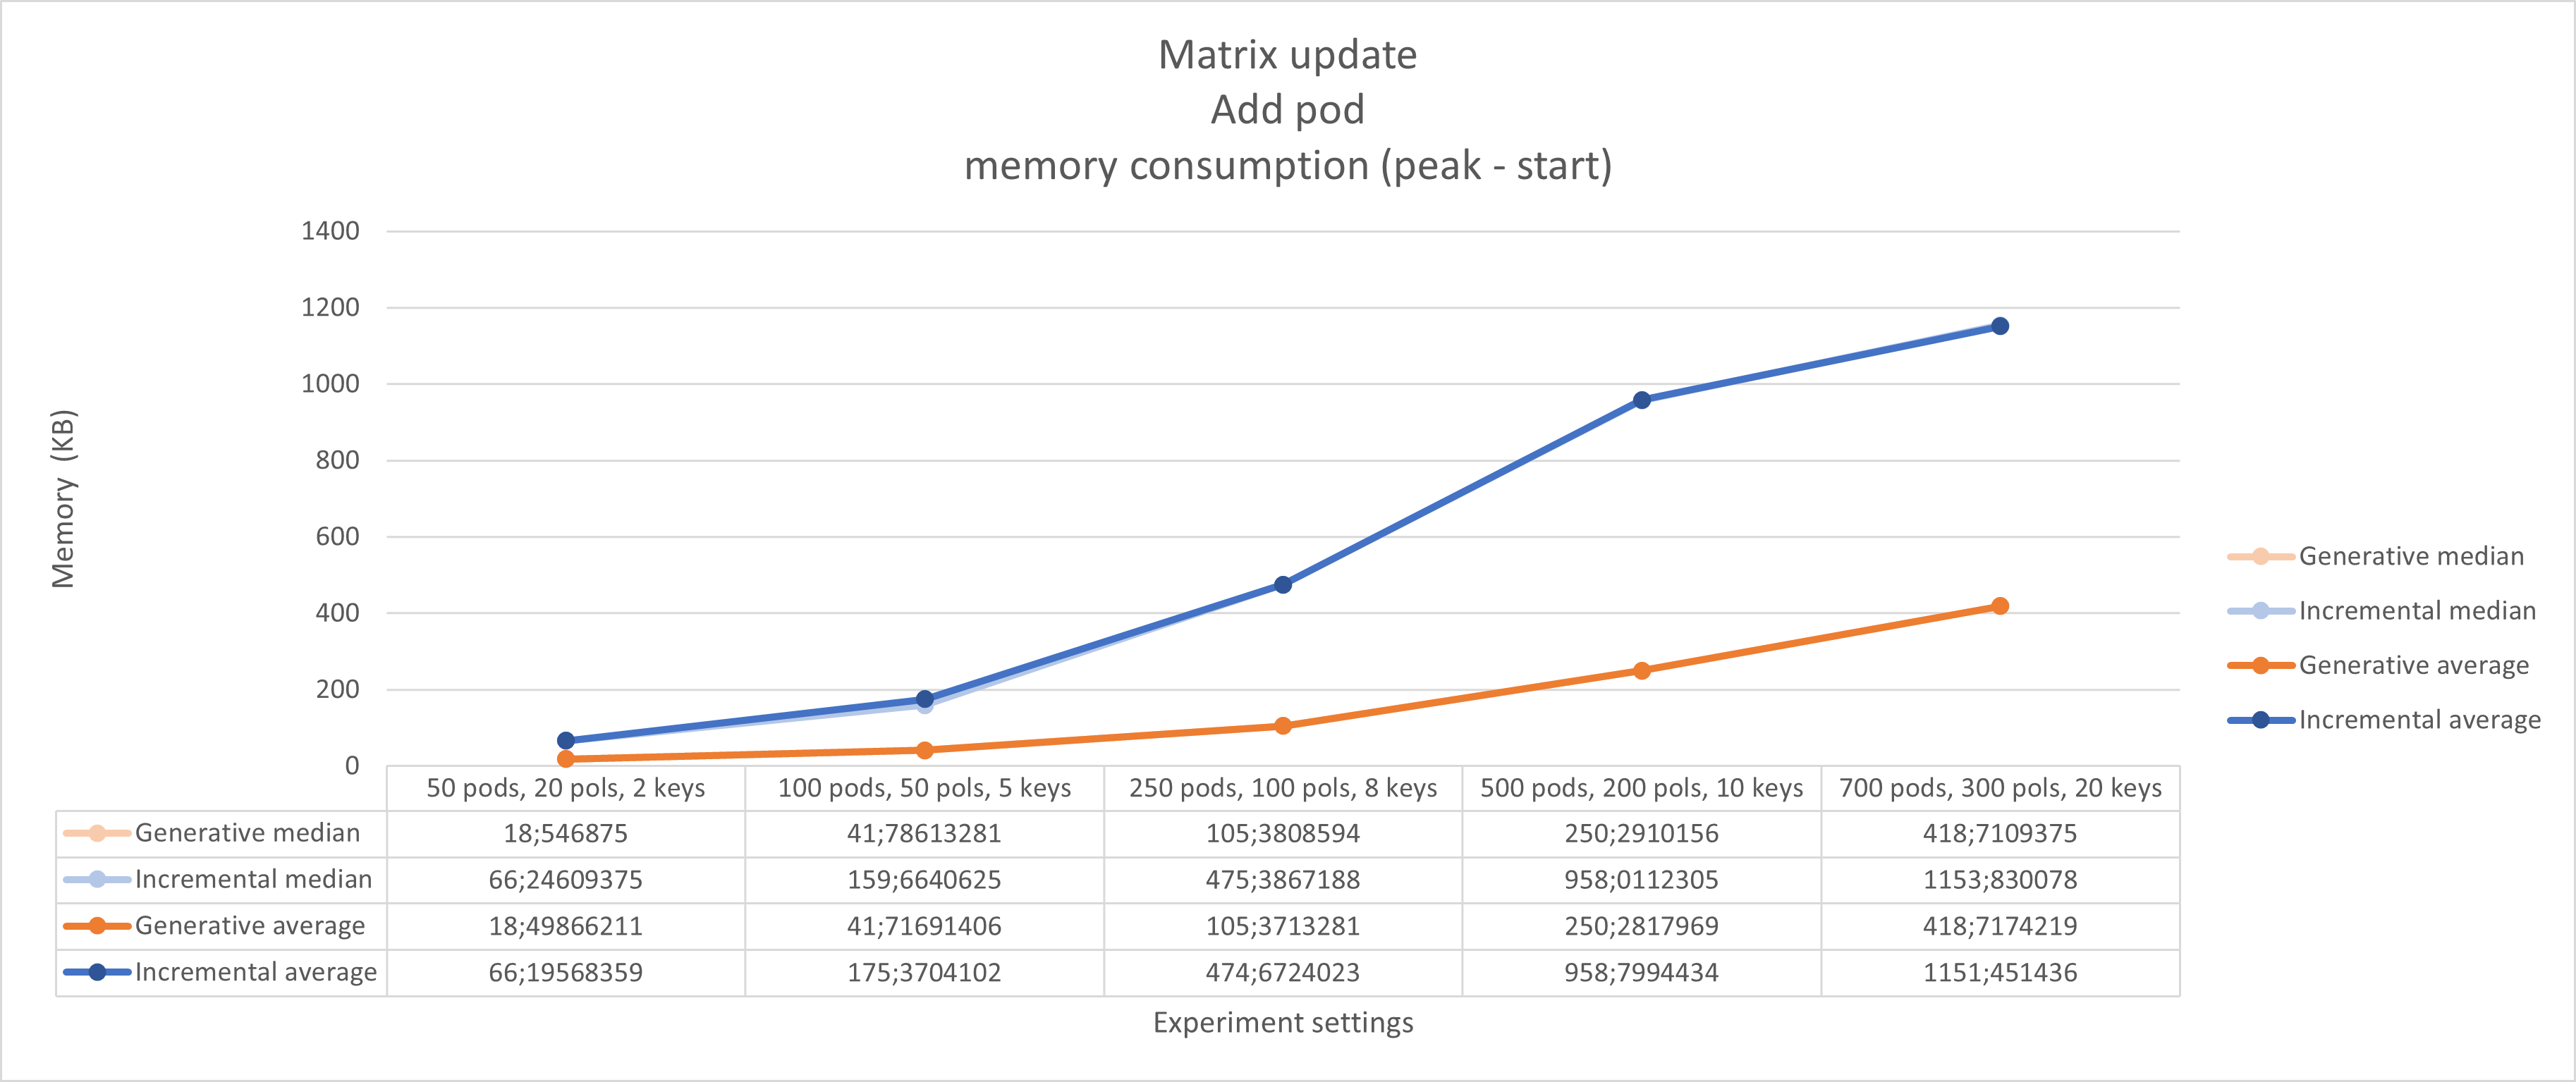
\includegraphics[width=\textwidth]{images/experiment1/addPod-memory.png}
    \caption{Memory consumption of adding a container}
    \label{fig:exp1-addPod-memory}
\end{figure}
\begin{figure}[H]
    \centering
    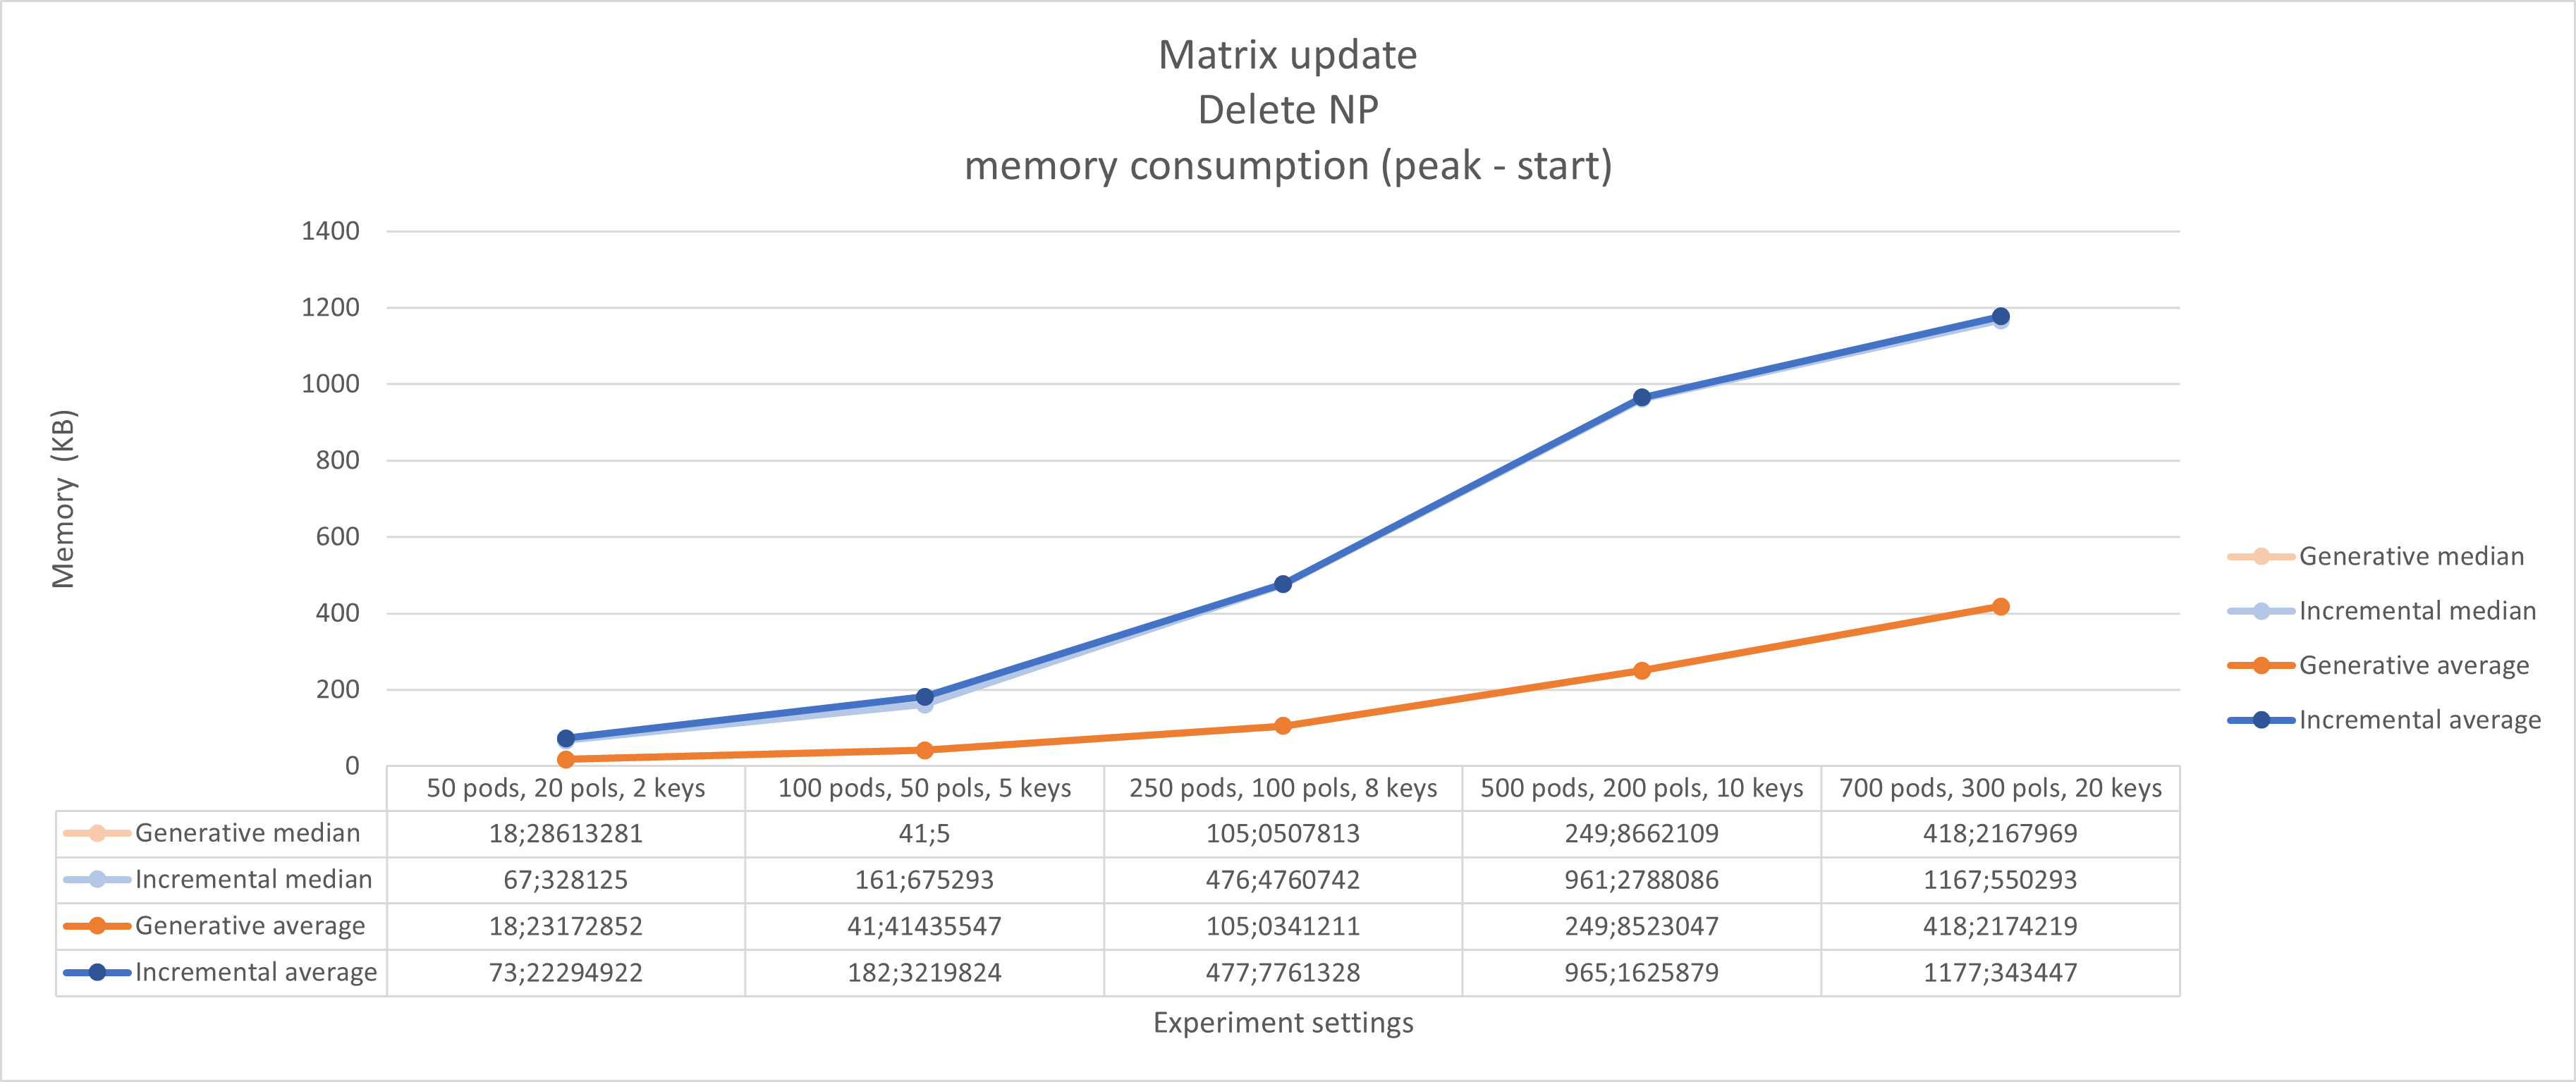
\includegraphics[width=\textwidth]{images/experiment1/delNP-memory.png}
    \caption{Memory consumption of deleting a network policy}
    \label{fig:exp1-delNP-memory}
\end{figure}
\begin{figure}[H]
    \centering
    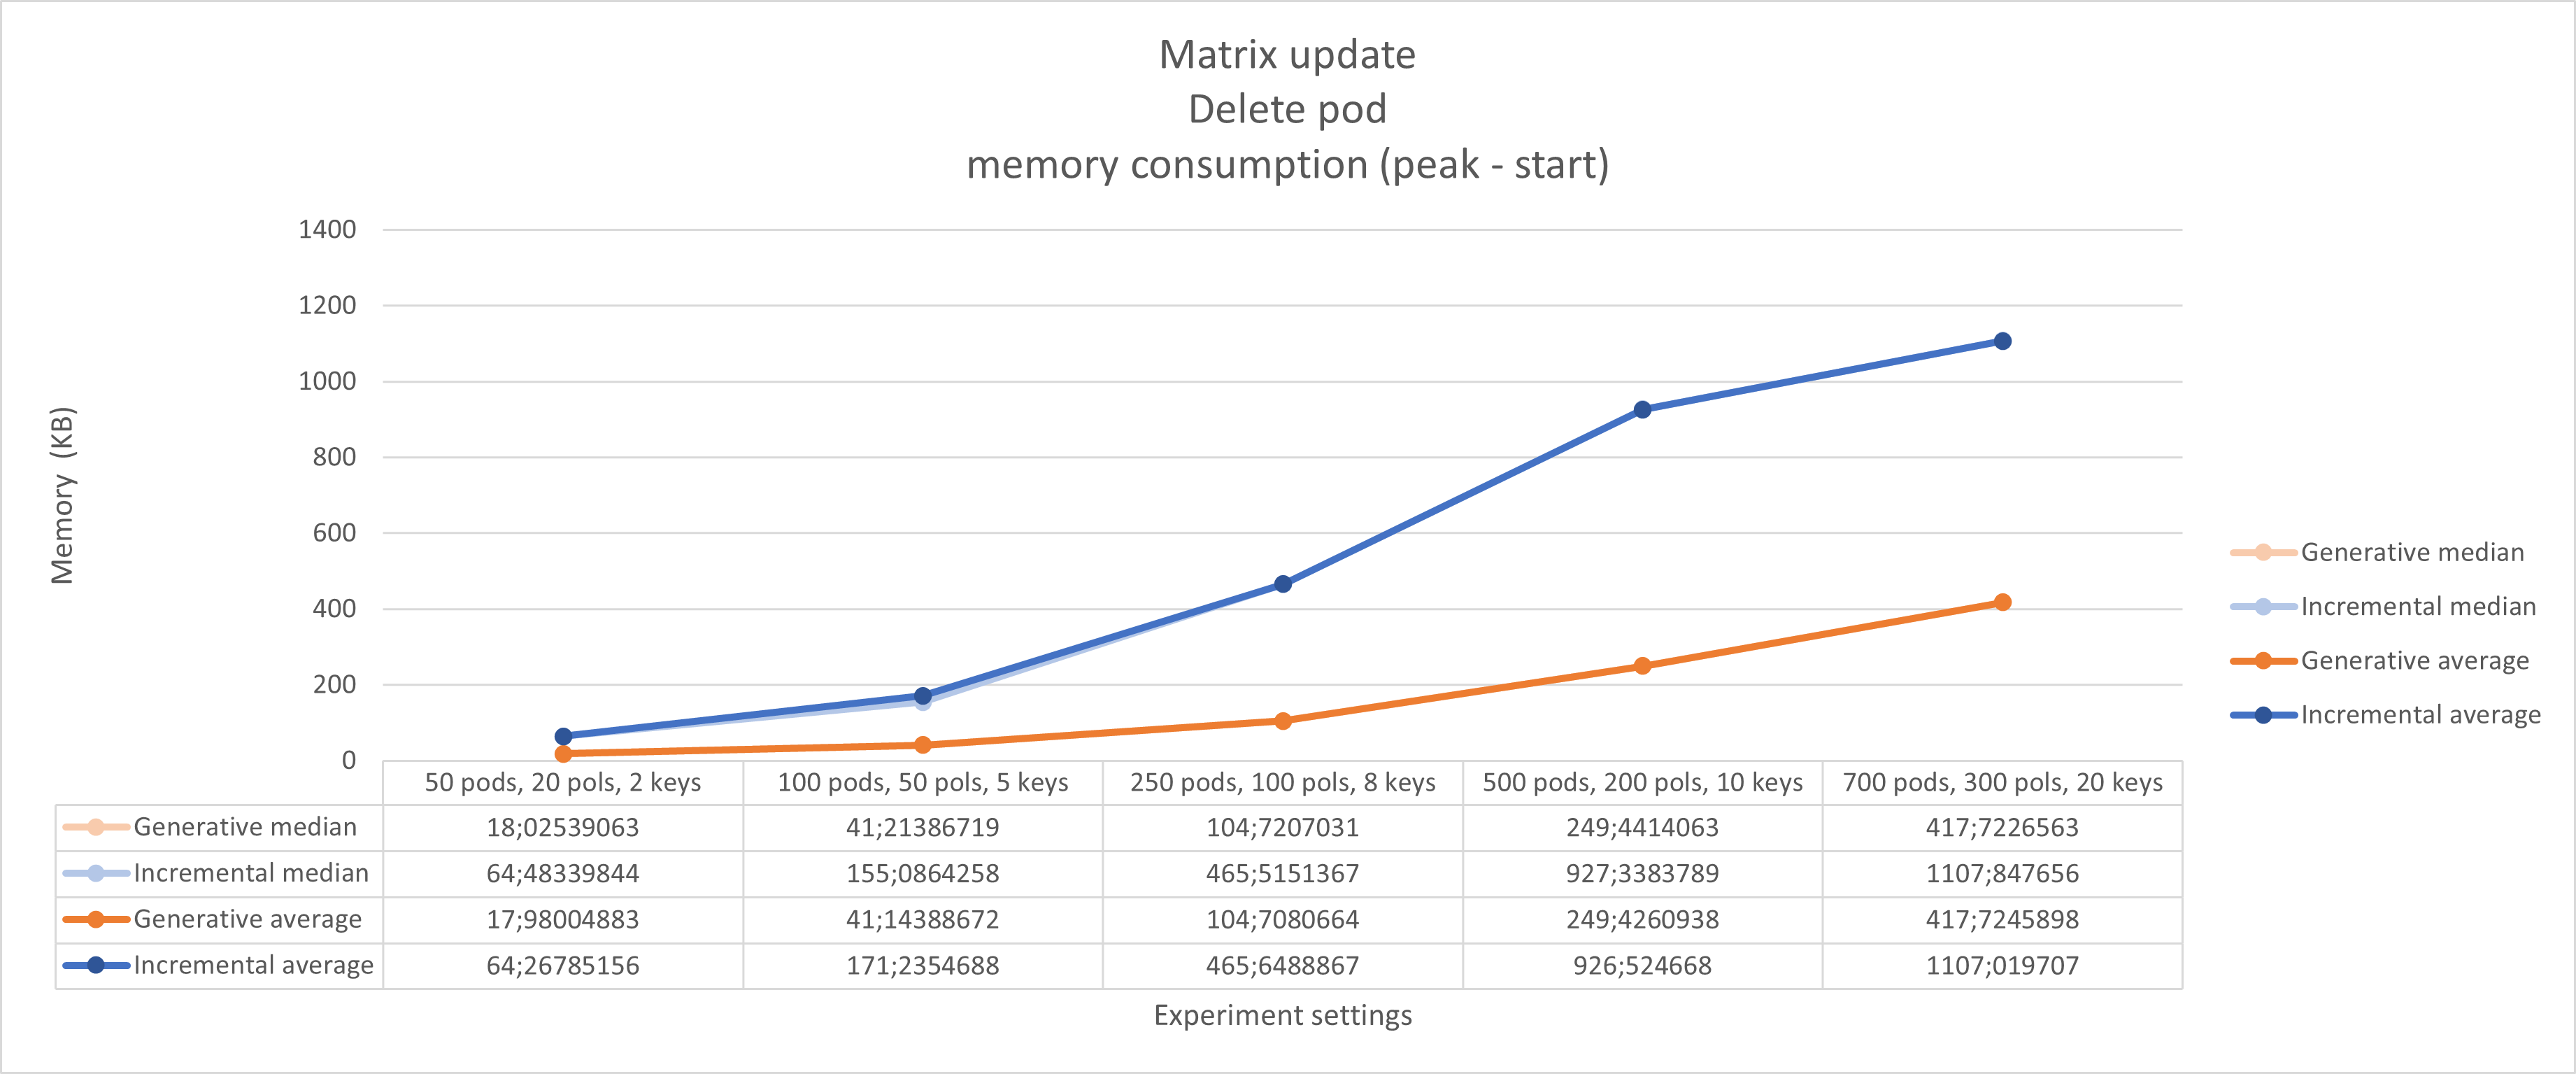
\includegraphics[width=\textwidth]{images/experiment1/delPod-memory.png}
    \caption{Memory consumption of deleting a container}
    \label{fig:exp1-delPod-memory}
\end{figure}



% ========================================================================================
\section{Experiment 2}\label{sec:experiment2}
The second experiment aims to give more insight into the overhead created by running our complete conflict detection algorithm on a cluster and will answer the following research questions:

\begin{itemize}
    \item \textit{Q3:} What is the relationship between pod/policy numbers and the time cost of conflict detection?
    \item \textit{Q4:} What is the relationship between pod/policy numbers and the space cost of conflict detection?
\end{itemize}

Before we delve into the experiment approach, setup and results we declare our hypotheses for these questions:

\begin{itemize}
    \item \textit{Hypothesis Q3:} We predict that the time that the algorithm takes will be lower than the average deployment time* of a pod, but that the time cost of our algorithm will increase as the cluster size increases.
    \item \textit{Hypothesis Q4:} We predict that the space cost of our algorithm will increase as the number of pods and network policies in the cluster increases as well.
\end{itemize}

* In the research paper of Grasshopper they found that t during their experiments the deployment time of an application can be up to 4 seconds in case of a cold start \cite{grashopper}. Since there is no default startup time for a container in a Kubernetes cluster we use this as a baseline.

% =========================================
\subsection{Approach} \label{exp2:approach}
For this experiment, we must use the entire algorithm instead of using a smaller part as we did in experiment 1. We can not compare our conflict detection, however, since there is no other research solution that provides the same functionality to the best of our knowledge. Instead, we measure general information about time and memory consumption when handling events. We once again use the same experiment setups as used in experiment 1 but must define additional parameters for the generation of the security groups and security group rules in the \acrshort{sgic} component. We will now describe the meaning of these additional parameters, while their values for this experiment can be seen in \autoref{tab:exp2pars}.

\begin{itemize}
    \item \textit{Nr of SG}: This constant describes the minimum and maximum amount of security groups that will be generated when initializing the \acrshort{sgic}. The exact amount of security groups are thus randomly selected between these values.
    \item \textit{Nr of SG rules }: This constant describes the minimum and maximum amount of security group rules that will be generated for each security group when initializing the \acrshort{sgic}. The exact amount of security group rules per \acrshort{sg} is thus randomly selected between these values.
    \item \textit{Nr of SG linked to node}: This constant describes the minimum and maximum amount of security groups that will be linked to a node. The exact amount of linked security groups is thus randomly selected between these values and is different for each node.
\end{itemize}

Lastly, we would like to mention that the variables within the security groups and security group rules are randomised as well. There is a 3\slash 5 chance that a \acrshort{sg} rule applies to a security group and a 2\slash 5 chance that it will specify an IP address. These IP addresses are randomised between 10 different values out of which 7 are the IPS of the nodes on the cluster to increase the chance of matching rules. 


\begin{table}[H]
    \centering
    \begin{tabular}{|l|c|c|c|c|c|}
        \hline
        \textbf{Name} & \textbf{setup 1} & \textbf{setup 2} & \textbf{setup 3} & \textbf{setup 4} & \textbf{setup 5}\\
        \hline
        Pod num & 50 & 100 & 250 & 500 & 750 \\
        Pol num & 20 & 50 & 100 & 200 & 300 \\
        Key limit & 2 & 5 & 8 & 10 & 20 \\
        Value limit & 10 & 10 & 10 & 10 & 10 \\
        Pol select limit & 1 & 1 & 1 & 1 & 1 \\
        Pol select label limit & 3 & 3 & 3 & 3 & 3 \\
        Pol allow limit & 3 & 3 & 3 & 3 & 3 \\
        Pol allow label limit & 3 & 3 & 3 & 3 & 3 \\
        Pod label limit & 5 & 5 & 5 & 5 & 5 \\
        Nr of SG & 6-16 & 6-16 & 6-16 & 6-16 & 6-16\\
        Nr of SG rules & 3-5 &3-5 & 3-5 & 3-5 & 3-5\\
        Nr of SG linked to node & 3-5 &3-5 & 3-5 & 3-5 & 3-5\\
	
        \hline
    \end{tabular}
    \caption{Experiment 2 parameter values}
    \label{tab:exp2pars}
\end{table}

The measurements retrieved from this experiment can be split into two parts: we analyze how long it takes for the watcher to get fully initialised and ready for capturing events, while also measuring the time and memory cost of our entire conflict detection algorithm in specific scenarios. For the first part of the experiment, we only retrieve the time between calling the watcher and it returning the ready status (ms). The second part is more extensive as we collect the time between applying an event and detection by the watcher (ms), the time it takes for conflict detection (ms) and lastly, the total time which is the combination of these last two (ms). 

% =========================================
\subsection{Execution} \label{exp2:execution}
The approach for this experiment is very similar to experiment 1 but with small yet very important changes.  We will now describe the execution of a single sub-experiment step by step where we will highlight the changes made in comparison with experiment 1.
\\[10pt]

\textbf{STEP 0:} Call the python file experiment2.py with the following arguments: $number\_of\_runs$, $number\_of\_pods$, $number\_of\_policies$, $namespace$, $key\_limit$ and $event\_type$ according to the sub-experiment settings. The algorithm will then execute STEP 1 to STEP 7 as many times as defined in argument $number\_of\_runs$.
\\[10pt]

\textbf{STEP 1:} We fully reset the namespace defined in the $namespace$ argument with the help of the Python Kubernetes API. This is coded in a separate delete.py file and extended with some extra tests and timeouts to guarantee that all objects are successfully removed before continuing.
\\[10pt]

\textbf{STEP 2:} We deploy as many pods and network policies as defined in arguments \newline $number\_of\_pods$ and $number\_of\_policies$. For this functionality a separate deploy.py python file has been created that will generate and deploy the network policies and pods, when called upon with the variables $namespace$ and $key\_limit$ as parameters. The other relevant constants in \autoref{tab:exp2pars} are hard coded since they don't change between sub-experiments. The deploy file is equipped with a list of distinct keys and values to leverage when creating the randomised pods and \acrshort{np}s. However, the key list is first shortened until it has a length equal to the $key\_limit$ parameter before being utilised. The randomised pods and network policies get deployed in the namespace defined in the $namespace$ argument with the help of the Python Kubernetes API. We use extra tests and timeouts to guarantee all objects are successfully deployed and ready before continuing. 
\textbf{We retrieve and store the current time and start the memory tracer}.
\\[10pt]

\textbf{STEP 3:} We start the watcher with the flags for debug mode,  verbose mode and start the checkup all set to False. With the use of threading events, we guarantee that the threads that watch the APIs for pods and \acrshort{np}s are successfully running, in order to prevent the next step from executing too early, therefore missing the event and being unable to handle it. \textbf{When the watcher returns that it is ready and monitoring the cluster we save the time and stop the memory tracer to store these for later evaluation}.
\\[10pt]

\textbf{STEP 4:} We execute one event, depending on the $event\_type$ argument. If it is a delete event we call the delete.py file again and let it randomly remove one of the existing objects that correspond to the event type. If it is a deploy event we call the deploy.py file to generate one more randomly generated object according to the correct parameters. \textbf{We save the time at which we send the API request to the Kubernetes API server}.
\\[10pt]

\textbf{STEP 5:} We once again leverage threading events to get notified when the consumer thread has received and handled its first event. Since the watcher was initialized after all pods and network policies were fully ready it will always be the event from step 4 that will be caught. When the consumer catches the event it will start the timer right before calling the analyzer for event handling. Once the analyzer returns the function call the timer immediately gets stopped to get a final execution time. Similarly, we measure the memory usage at the start of the algorithm, and the highest peak of memory usage during the event handling. With this we can calculate the difference and thus how much memory was used (in bytes). These memory and time measurements get stored in variables in the watcher.
\\[10pt]

\textbf{STEP 6:} Once we get the message that the event is handled we retrieve the measurements from the watcher and store it locally. We can then stop the watcher. 
\textbf{This includes the time at which the event was detected by the watcher.} \textbf{With all the time measurements that we collected we calculate some usable values such as the time between the Kubernetes API call and event detection, and the total time between the Kubernetes API call and completion of conflict detection}.
\\[10pt]

\textbf{STEP 7:} Once the hundred runs of the sub-experiment have finished we store all the data in a CSV file and store it on the control plane node that ran the experiment. We can then retrieve this file and combine it with other sub-experiment files for evaluation.  \textbf{Since there is no comparison in experiment 2 step 7 equals to step 8 of experiment 1}. 
\\[10pt]


% =========================================
\subsection{Experiment results} \label{exp2:results}
Similarly to experiment 1 we created two graphs for each of the four captured events: one for the average and median time and the other for the average and median memory consumption. When comparing the graphs with experiment 1 we can see that there are only two data lines instead of four since there is only a single update method of the reachabilitymatrix used. Additionally, the graphs show data for the entire conflict detection solution instead of solely the update of the reachabilitymatrix. Aside from these 8 event graphs we also have two graphs regarding the time and memory consumption of the startup process of the watcher which is defined as the period between execution of the script up until the point at which the algorithm is readily monitoring the cluster. This startup data thus includes initialization of variables, reachabilitymatrix generation, cloud layer generation and setting up multithreaded API monitors. In these startup graphs, we do not separate the data per event since the event has not occurred yet when the algorithm is initialized and thus has no influence. Please note that the conflict detection graphs all use the same values and increments on their axis to allow a direct comparison, but the startup graph does not follow this promise: it shows the time in seconds instead of milliseconds. We will start by looking at the startup graphs after which we continue with the time and memory graphs for conflict detection.
\\[10pt]

\textbf{Watcher Startup}
\newline The time and memory consumption for initialising the watcher can be seen in \autoref{fig:exp2-startup-time} and \autoref{fig:exp2-startup-memory} respectively. The goal of these graphs is to give a general sense of resource consumption for the algorithm's startup phase, but we have no hard time limit imposed since the algorithm should in theory only be started once, and usually in a non-time-sensitive environment. We can deduct two interesting conclusions from the graphs:

\begin{itemize}
    	\item The median time deviates from the average time, which we attribute once again to the idea that the amount of connections in the cluster setup directly influences the speed of our solution. This difference increases with cluster size since more network policies and containers directly translate to a higher chance of container connection.
	\item The memory consumption shows no surprises nor does it show any significant difference between the average and mean values, indicating that our algorithm remains very stable. Interestingly enough this indicates that variables whose size depends on the number of allowed connections, such as resp\_policies  in the reachability structure (see \autoref{impl:model}) do not have much influence on the total memory consumption.

\end{itemize}

\begin{figure}[H]
    \centering
    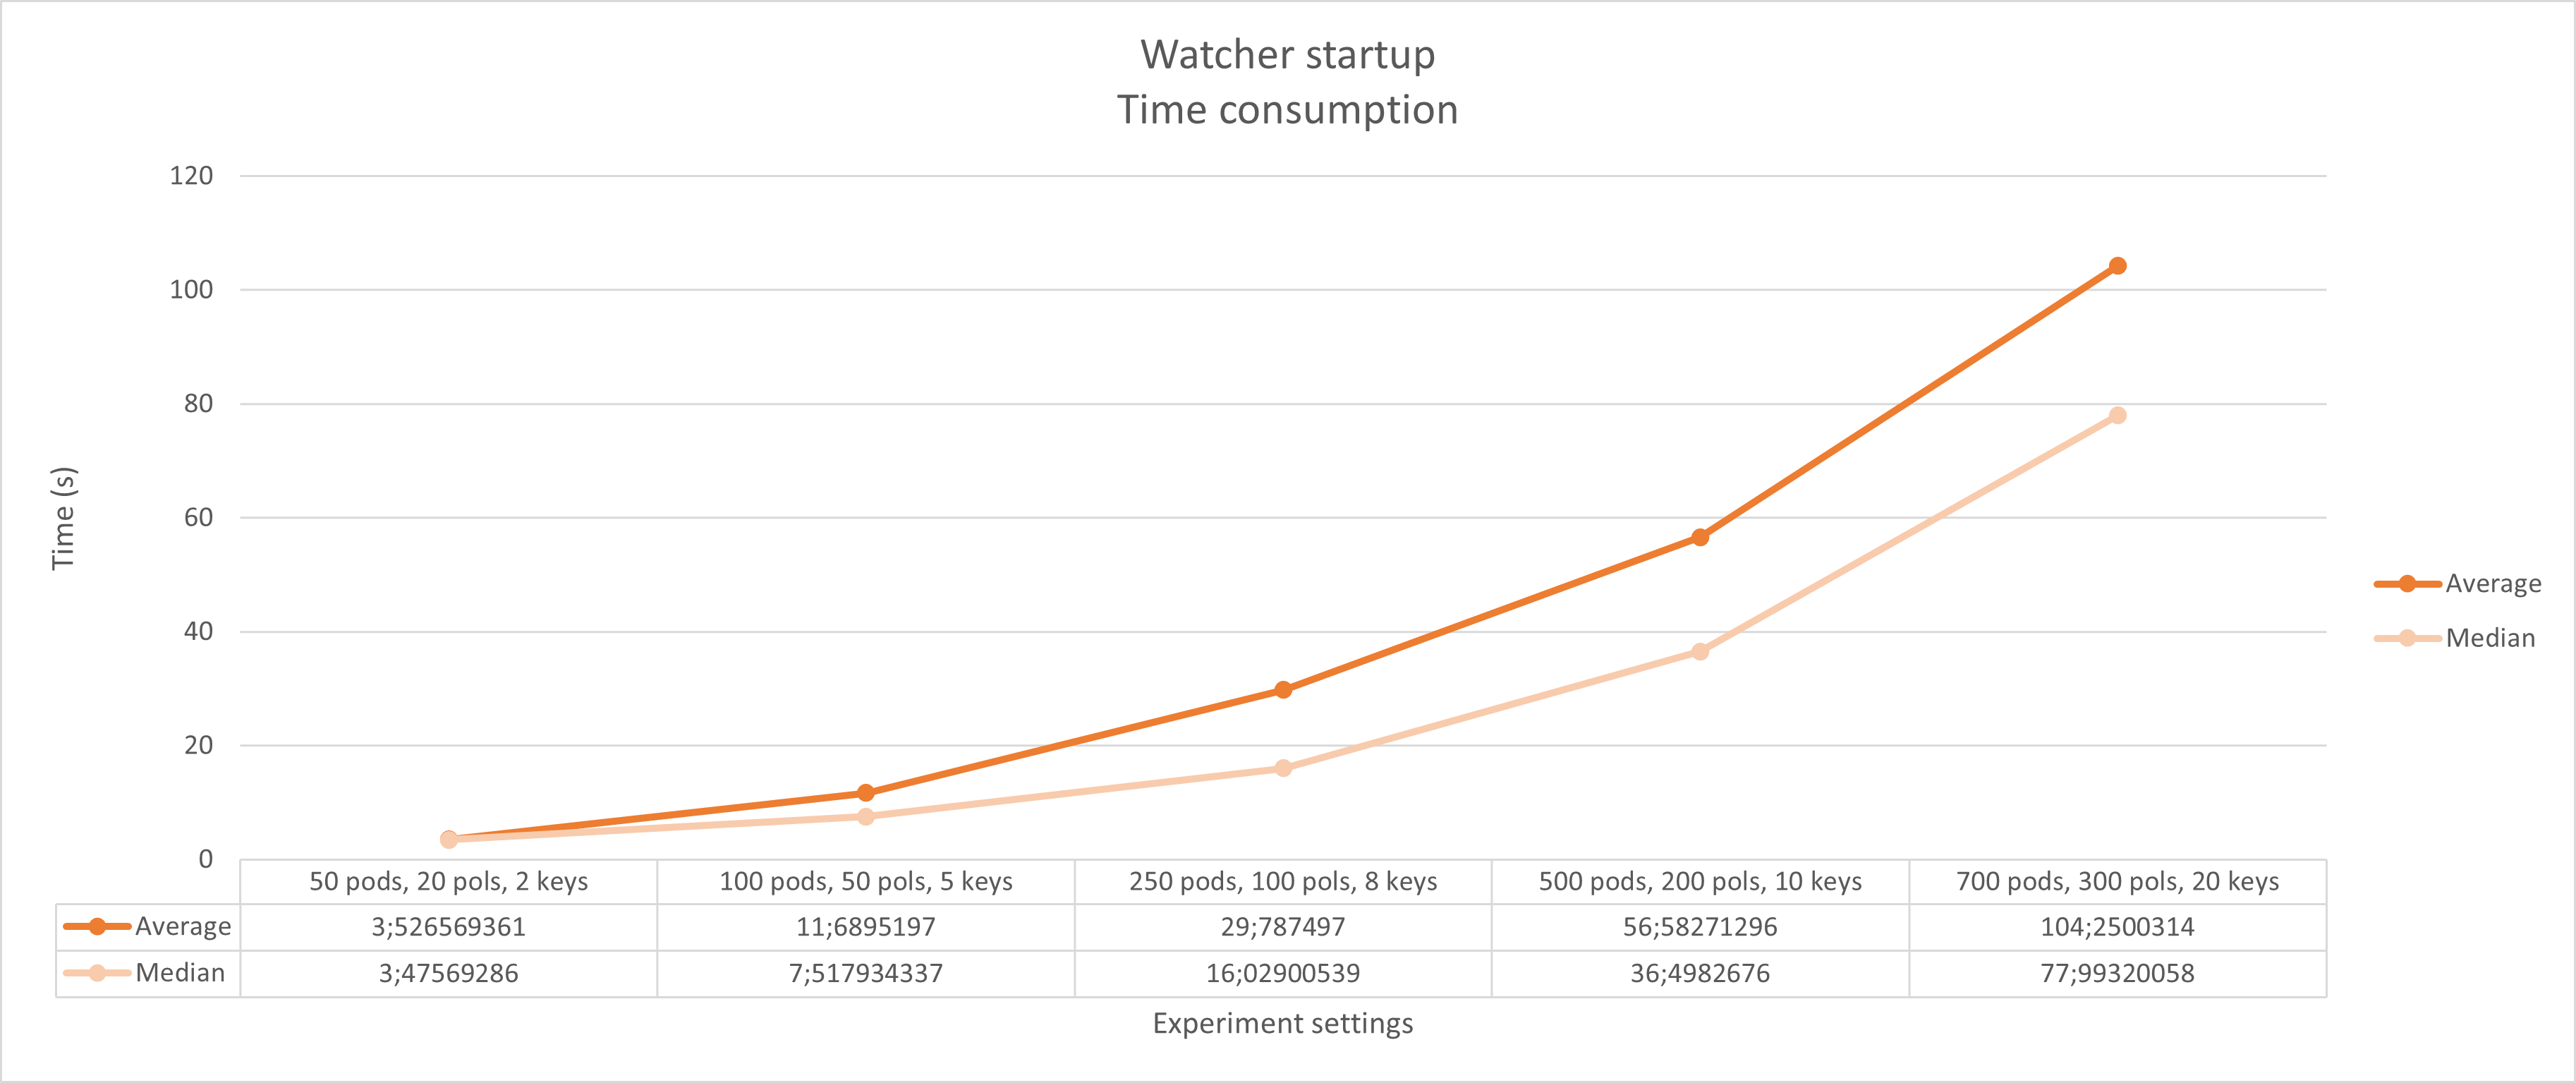
\includegraphics[width=\textwidth]{images/experiment2/watcher-startup-time.png}
    \caption{Time consumption of starting up the algorithm}
    \label{fig:exp2-startup-time}
\end{figure}
\begin{figure}[H]
    \centering
    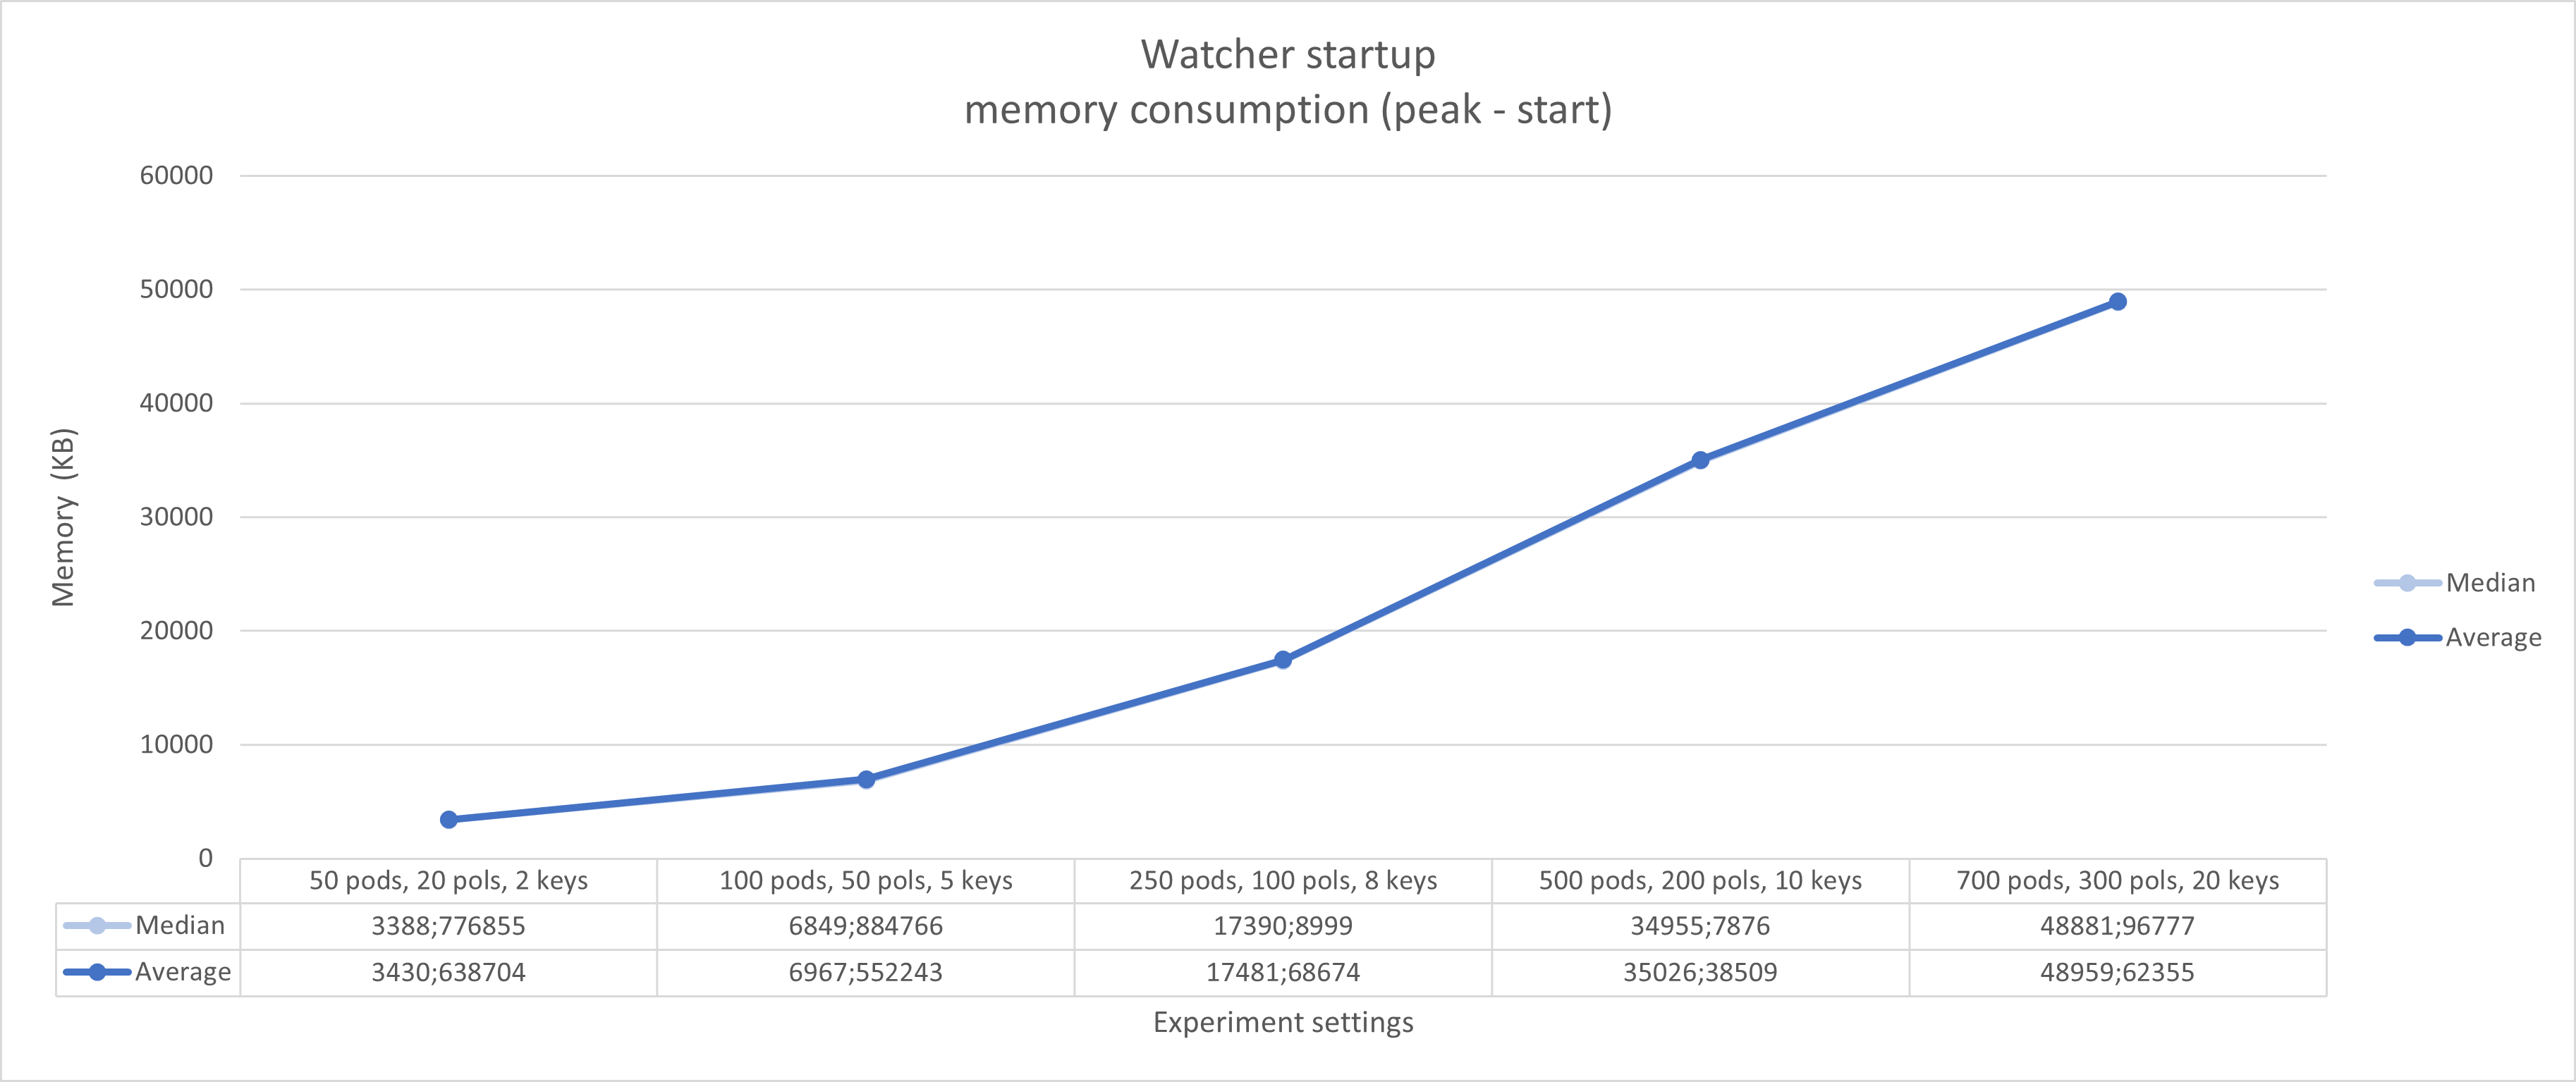
\includegraphics[width=\textwidth]{images/experiment2/watcher-startup-memory.png}
    \caption{Memory consumption of starting up the algorithm}
    \label{fig:exp2-startup-memory}
\end{figure}



\textbf{Time consumption}
\newline The time consumption for the full conflict detection solution for each of the four events are shown in \autoref{fig:exp2-addNP-time-conflict}, \autoref{fig:exp2-addPod-time-conflict}, \autoref{fig:exp2-delNP-time-conflict} and \autoref{fig:exp2-delPod-time-conflict}.  We can see that the conflict detection time remains safely below the 4-second pod deployment threshold stated in the hypothesis for Q3 with the highest average being 474ms for the deletion of a network policy. Furthermore, we can deduct some interesting information from the graphs:
\begin{itemize}
    \item For each of the events and cluster setup combinations the median value lies lower than the average value, indicating the presence of high values that pull the average up. We once again assume this is related to the amount of container connections.
    \item When we compare the graphs for experiment 2 to the incremental approach of the corresponding event graphs in experiment 1 we see that the incremental approach for updating the reachabilitymatrix is the main contributor to time consumption, while the conflict detection only adds a slight overhead.
\end{itemize}

\begin{figure}[H]
    \centering
    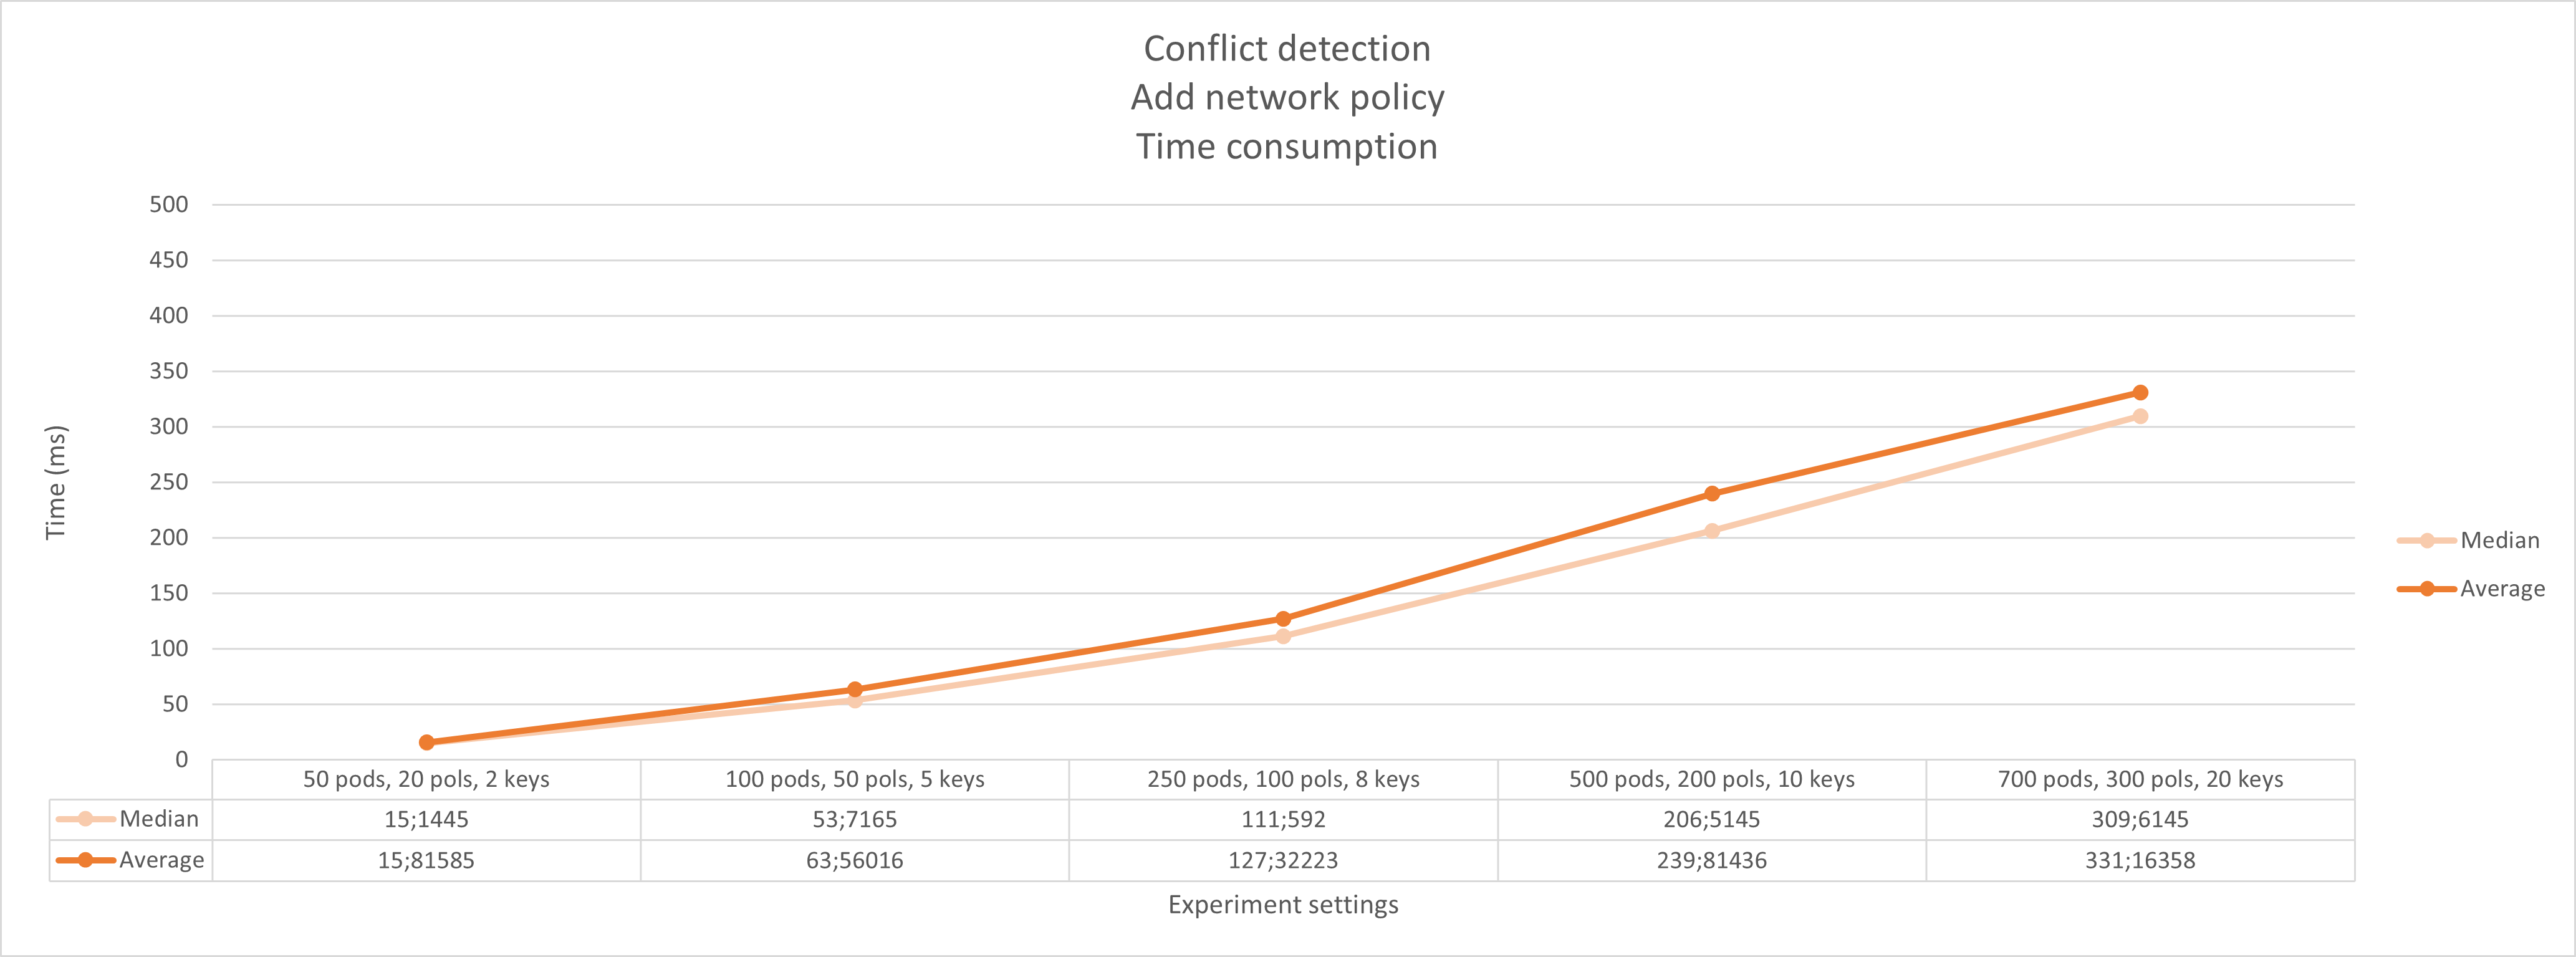
\includegraphics[width=\textwidth]{images/experiment2/addNP-time-conflict.png}
    \caption{conflict detection time consumption - add network policy}
    \label{fig:exp2-addNP-time-conflict}
\end{figure}
\begin{figure}[H]
    \centering
    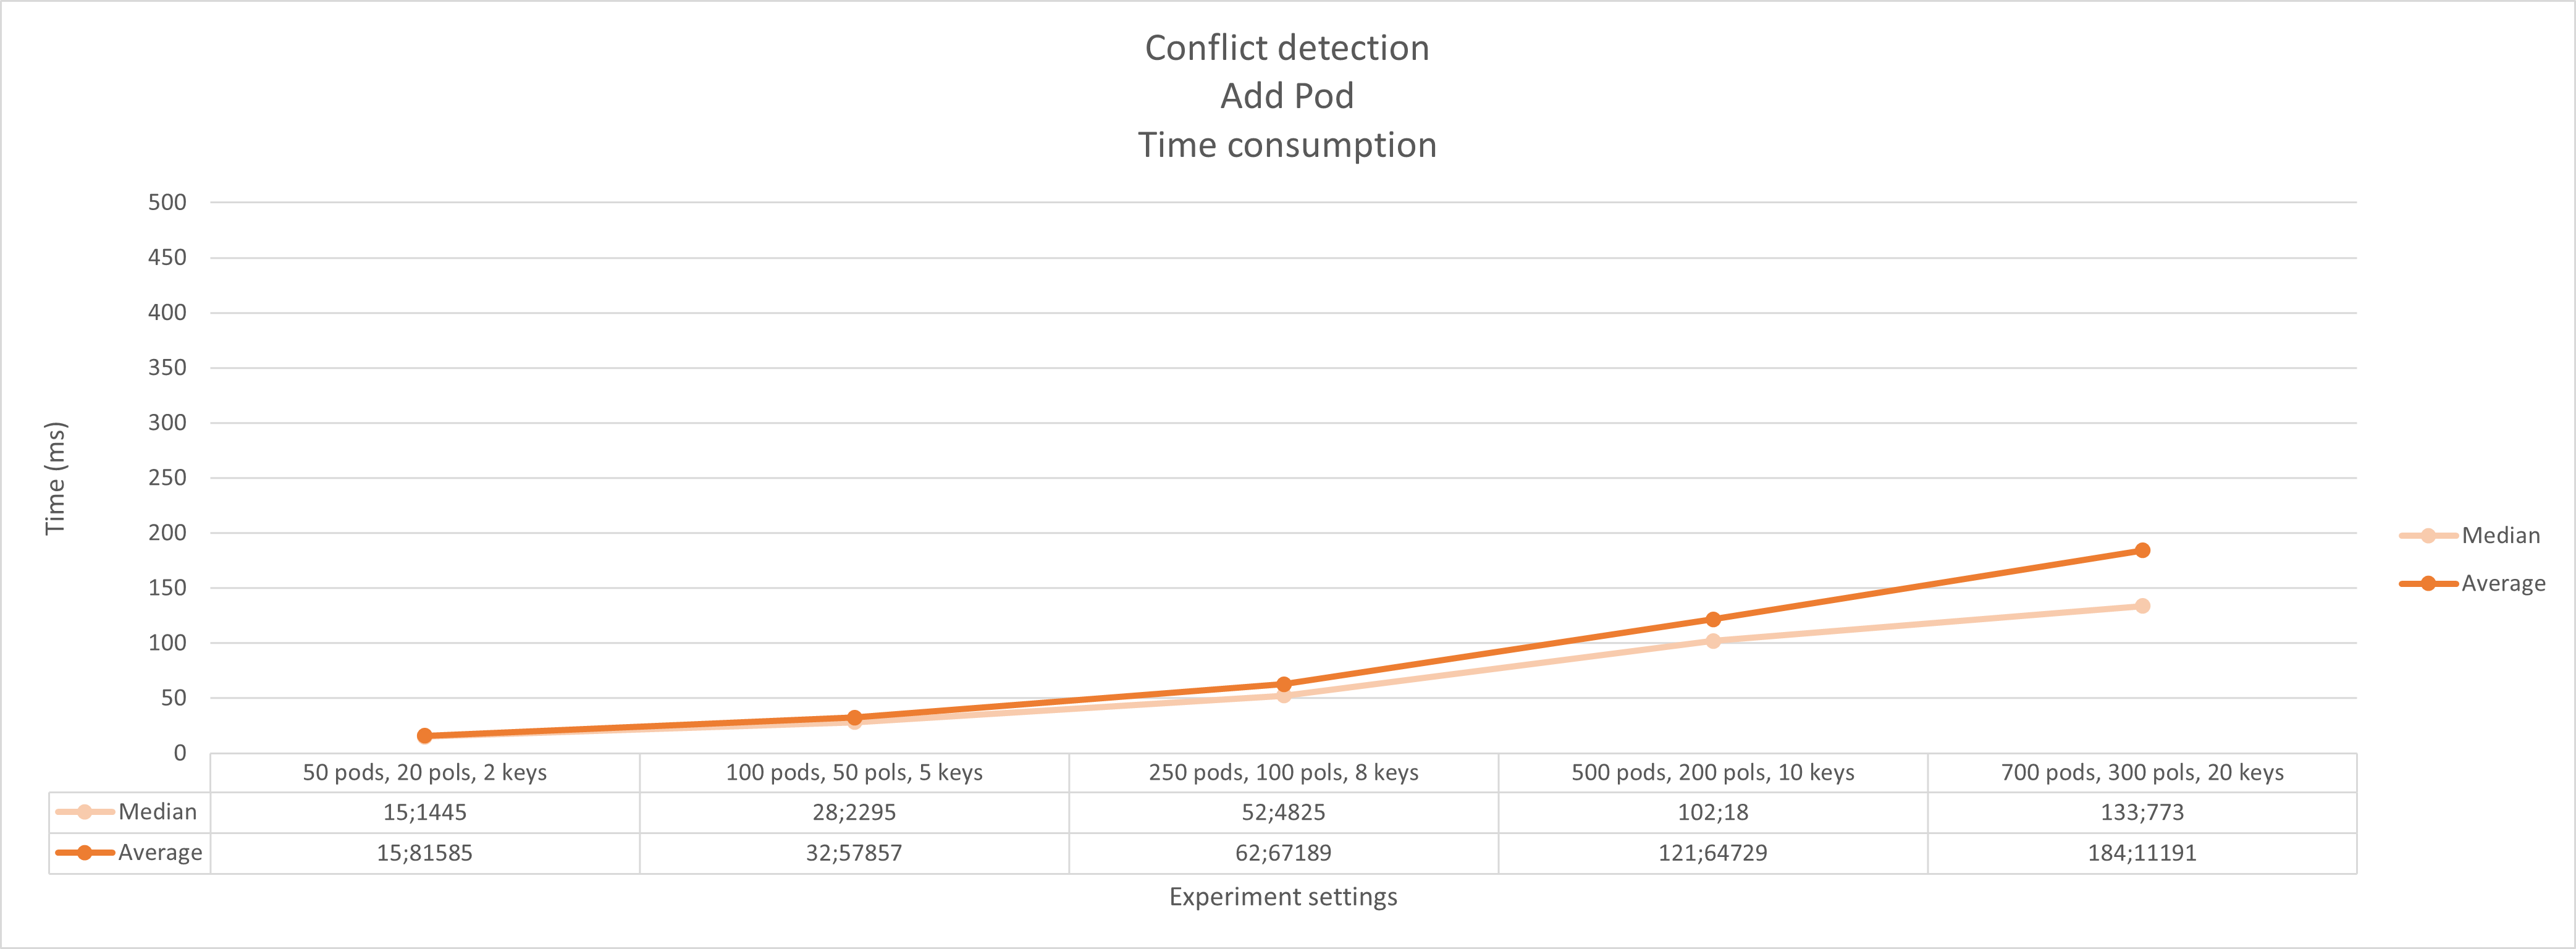
\includegraphics[width=\textwidth]{images/experiment2/addPod-time-conflict.png}
    \caption{conflict detection time consumption - add container}
    \label{fig:exp2-addPod-time-conflict}
\end{figure}
\begin{figure}[H]
    \centering
    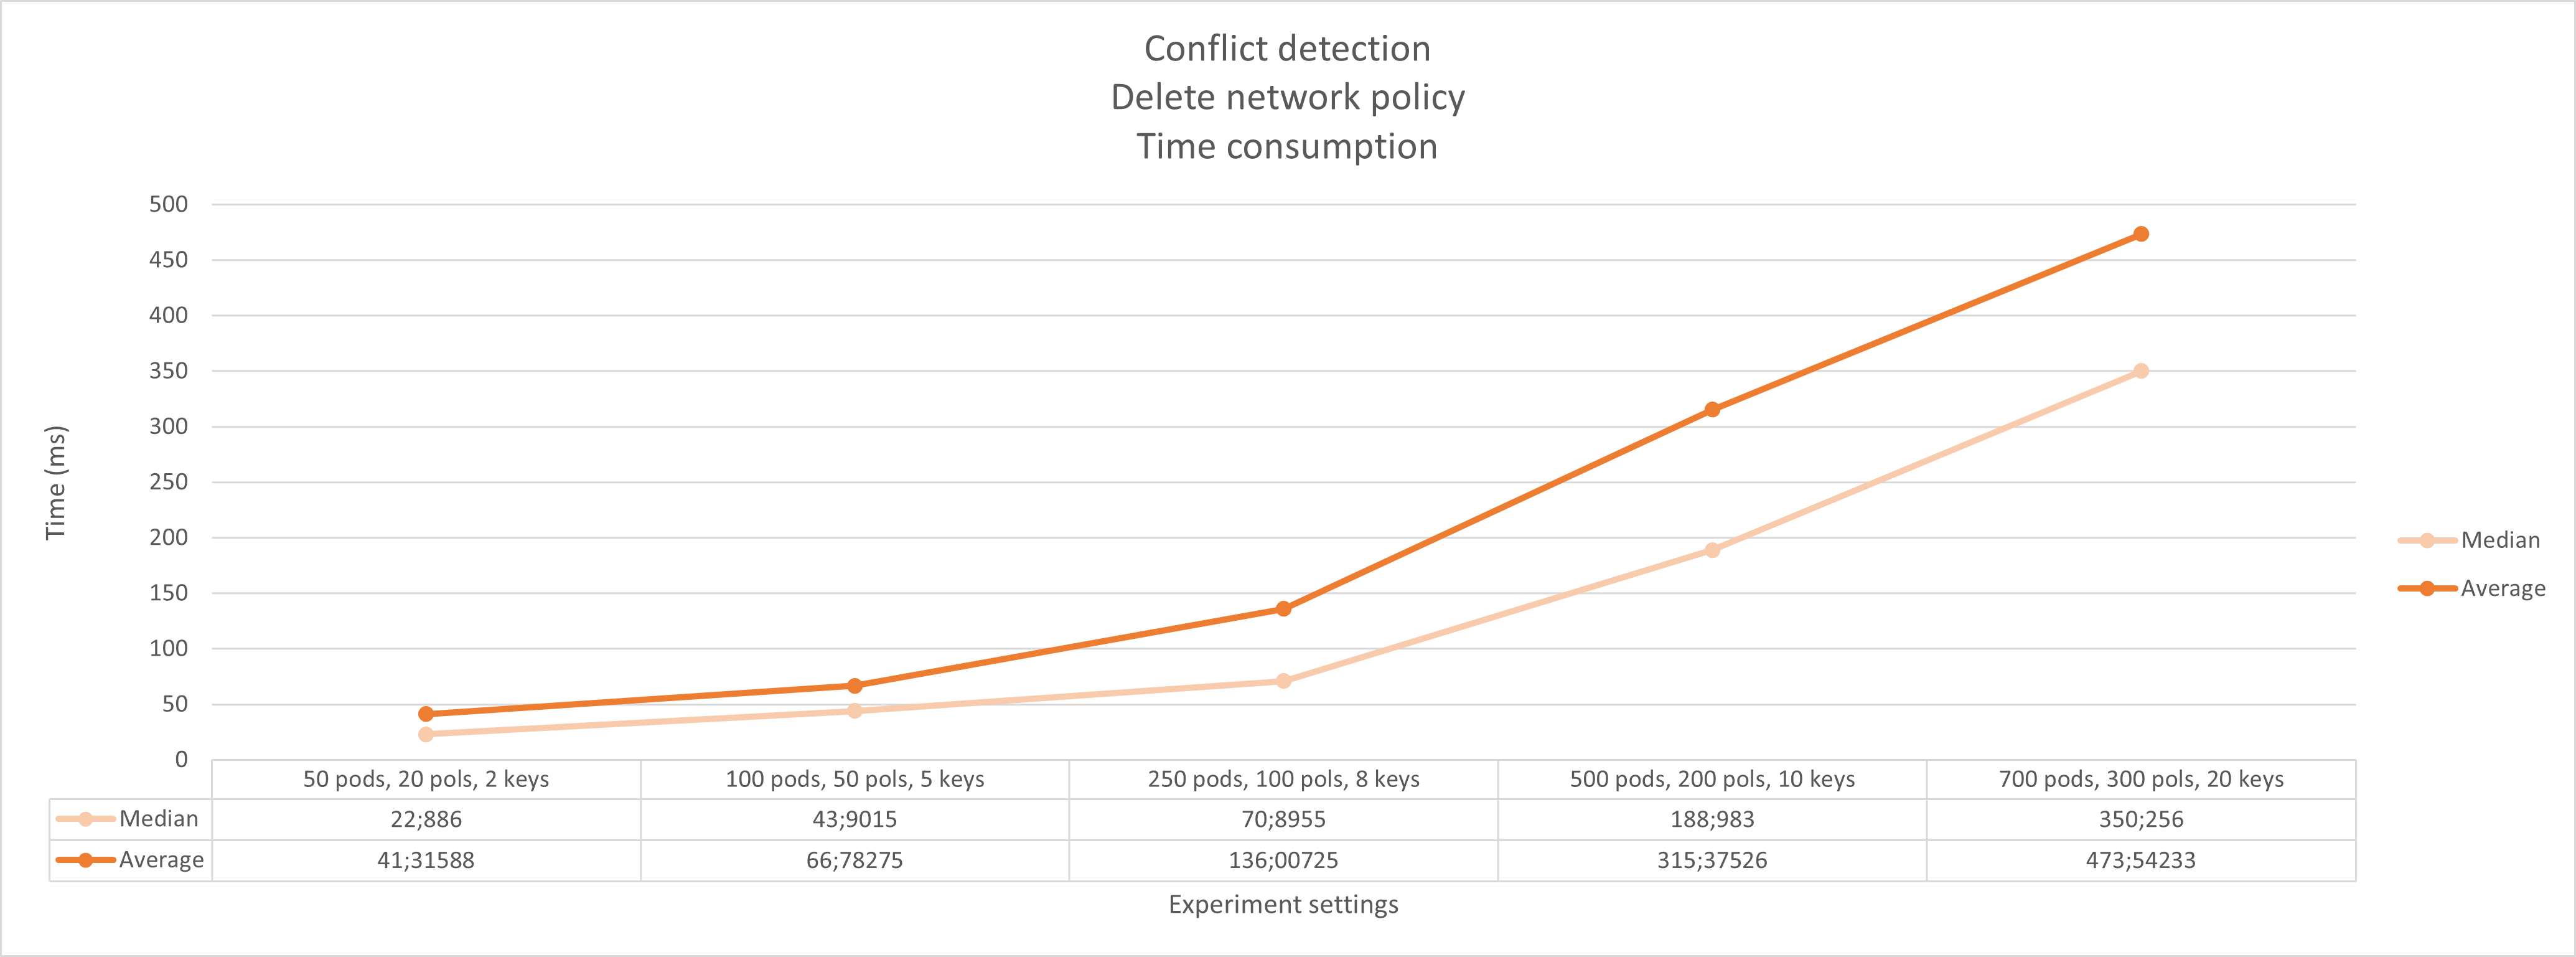
\includegraphics[width=\textwidth]{images/experiment2/delNP-time-conflict.png}
    \caption{conflict detection time consumption - delete network policy}
    \label{fig:exp2-delNP-time-conflict}
\end{figure}
\begin{figure}[H]
    \centering
    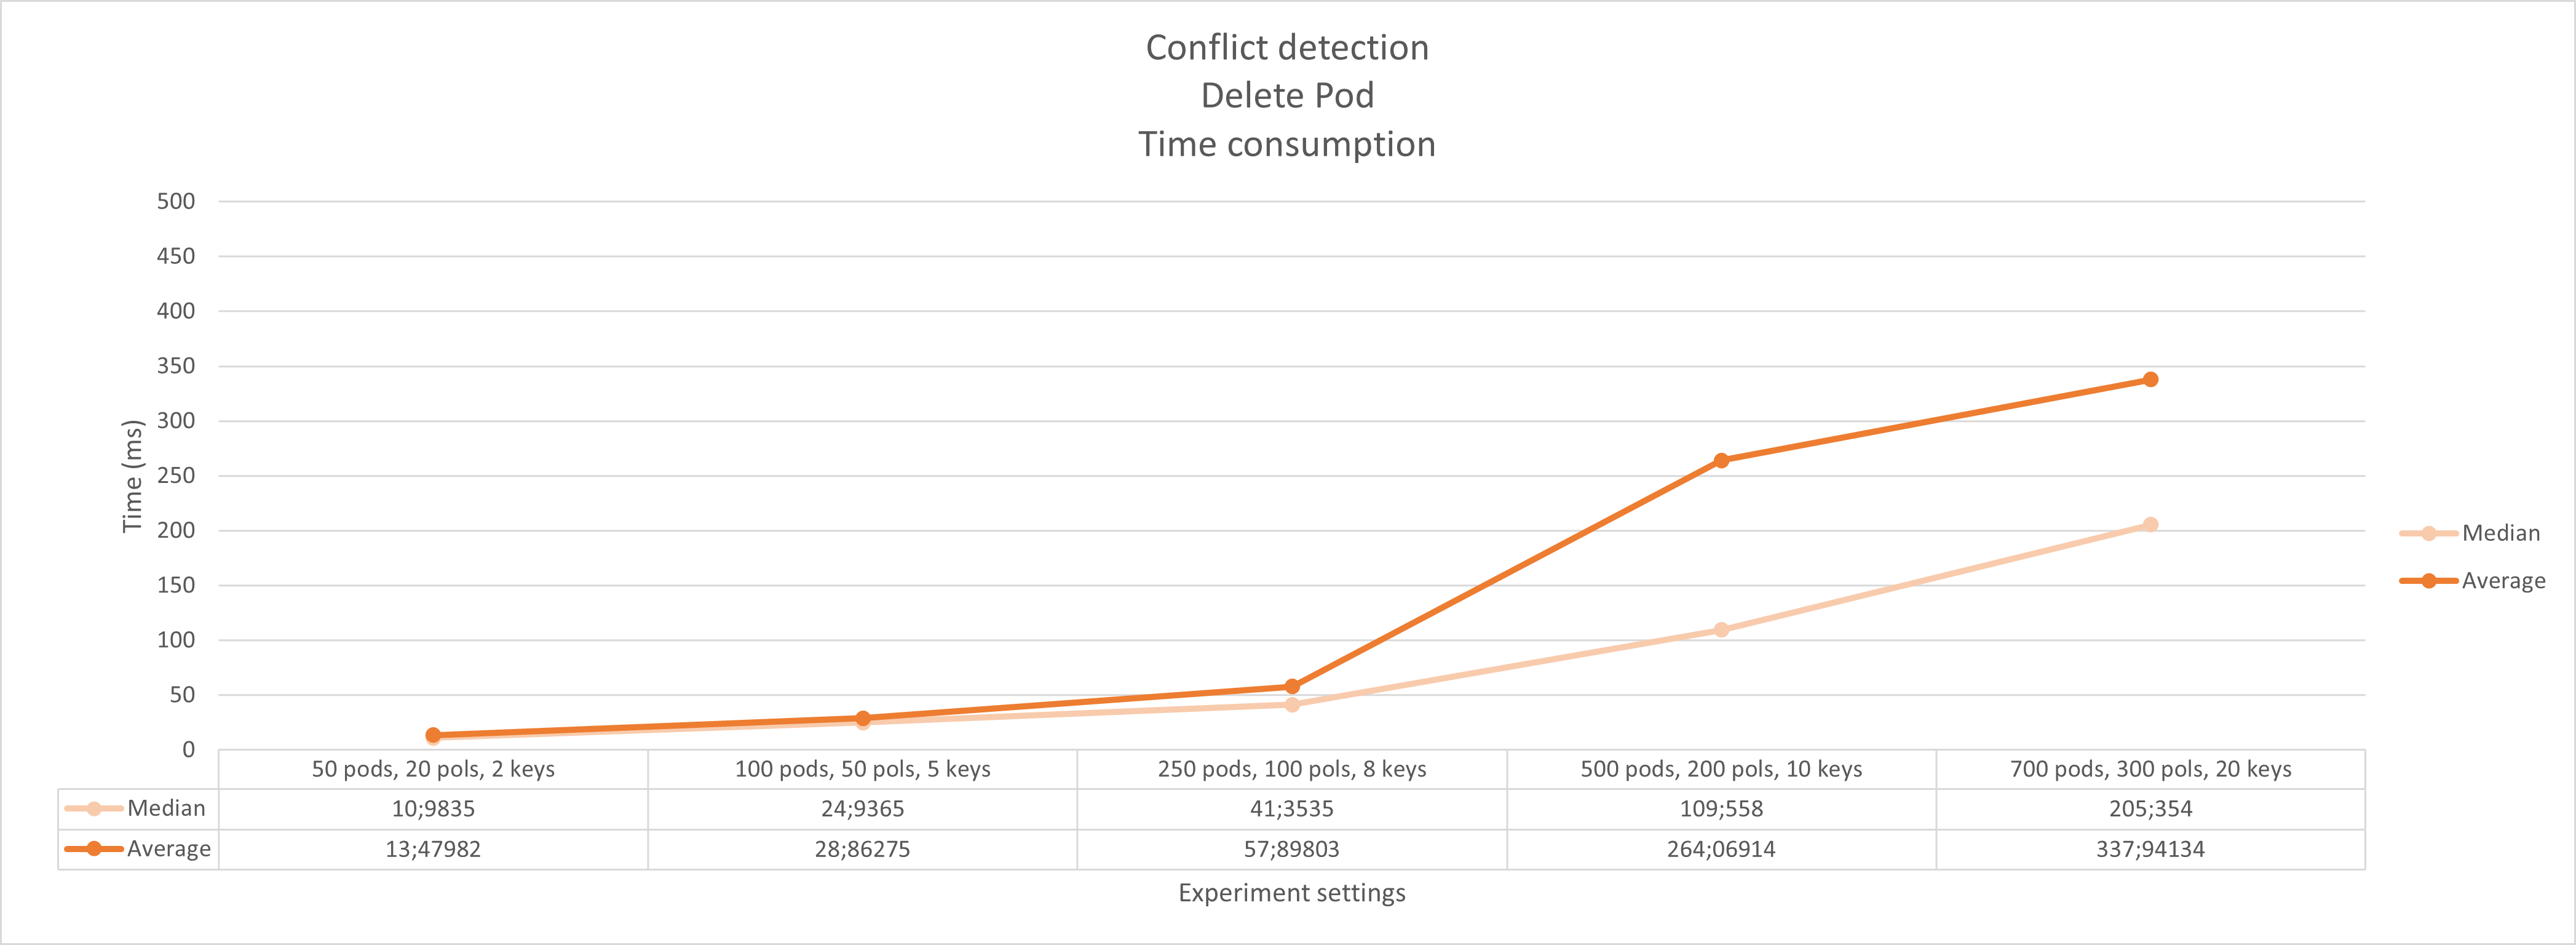
\includegraphics[width=\textwidth]{images/experiment2/delPod-time-conflict.png}
    \caption{conflict detection time consumption - delete container}
    \label{fig:exp2-delPod-time-conflict}
\end{figure}



\textbf{Memory consumption}
\newline The memory consumption for the full conflict detection solution for each of the four events are shown in \autoref{fig:exp2-addNP-memory-conflict}, \autoref{fig:exp2-addPod-memory-conflict}, \autoref{fig:exp2-delNP-memory-conflict} and \autoref{fig:exp2-delPod-memory-conflict}. The average values are usually in line with the median values meaning little to no skewing of data occurs due to outliers. One exception is the addition of a network policy where the median lies higher than the average, which was also visible in the corresponding graph in experiment 1. We, therefore, assume that this is due to the incremental update of the cluster state and not because of the conflict detection itself, although an exact reason could not be found and would require extra experimentation. We conclude that some small differences between events can be found but there are no specific outliers that catch the attention and that the memory increases as the cluster grows in size which is in line with our hypothesis for Q4.

\begin{figure}[H]
    \centering
    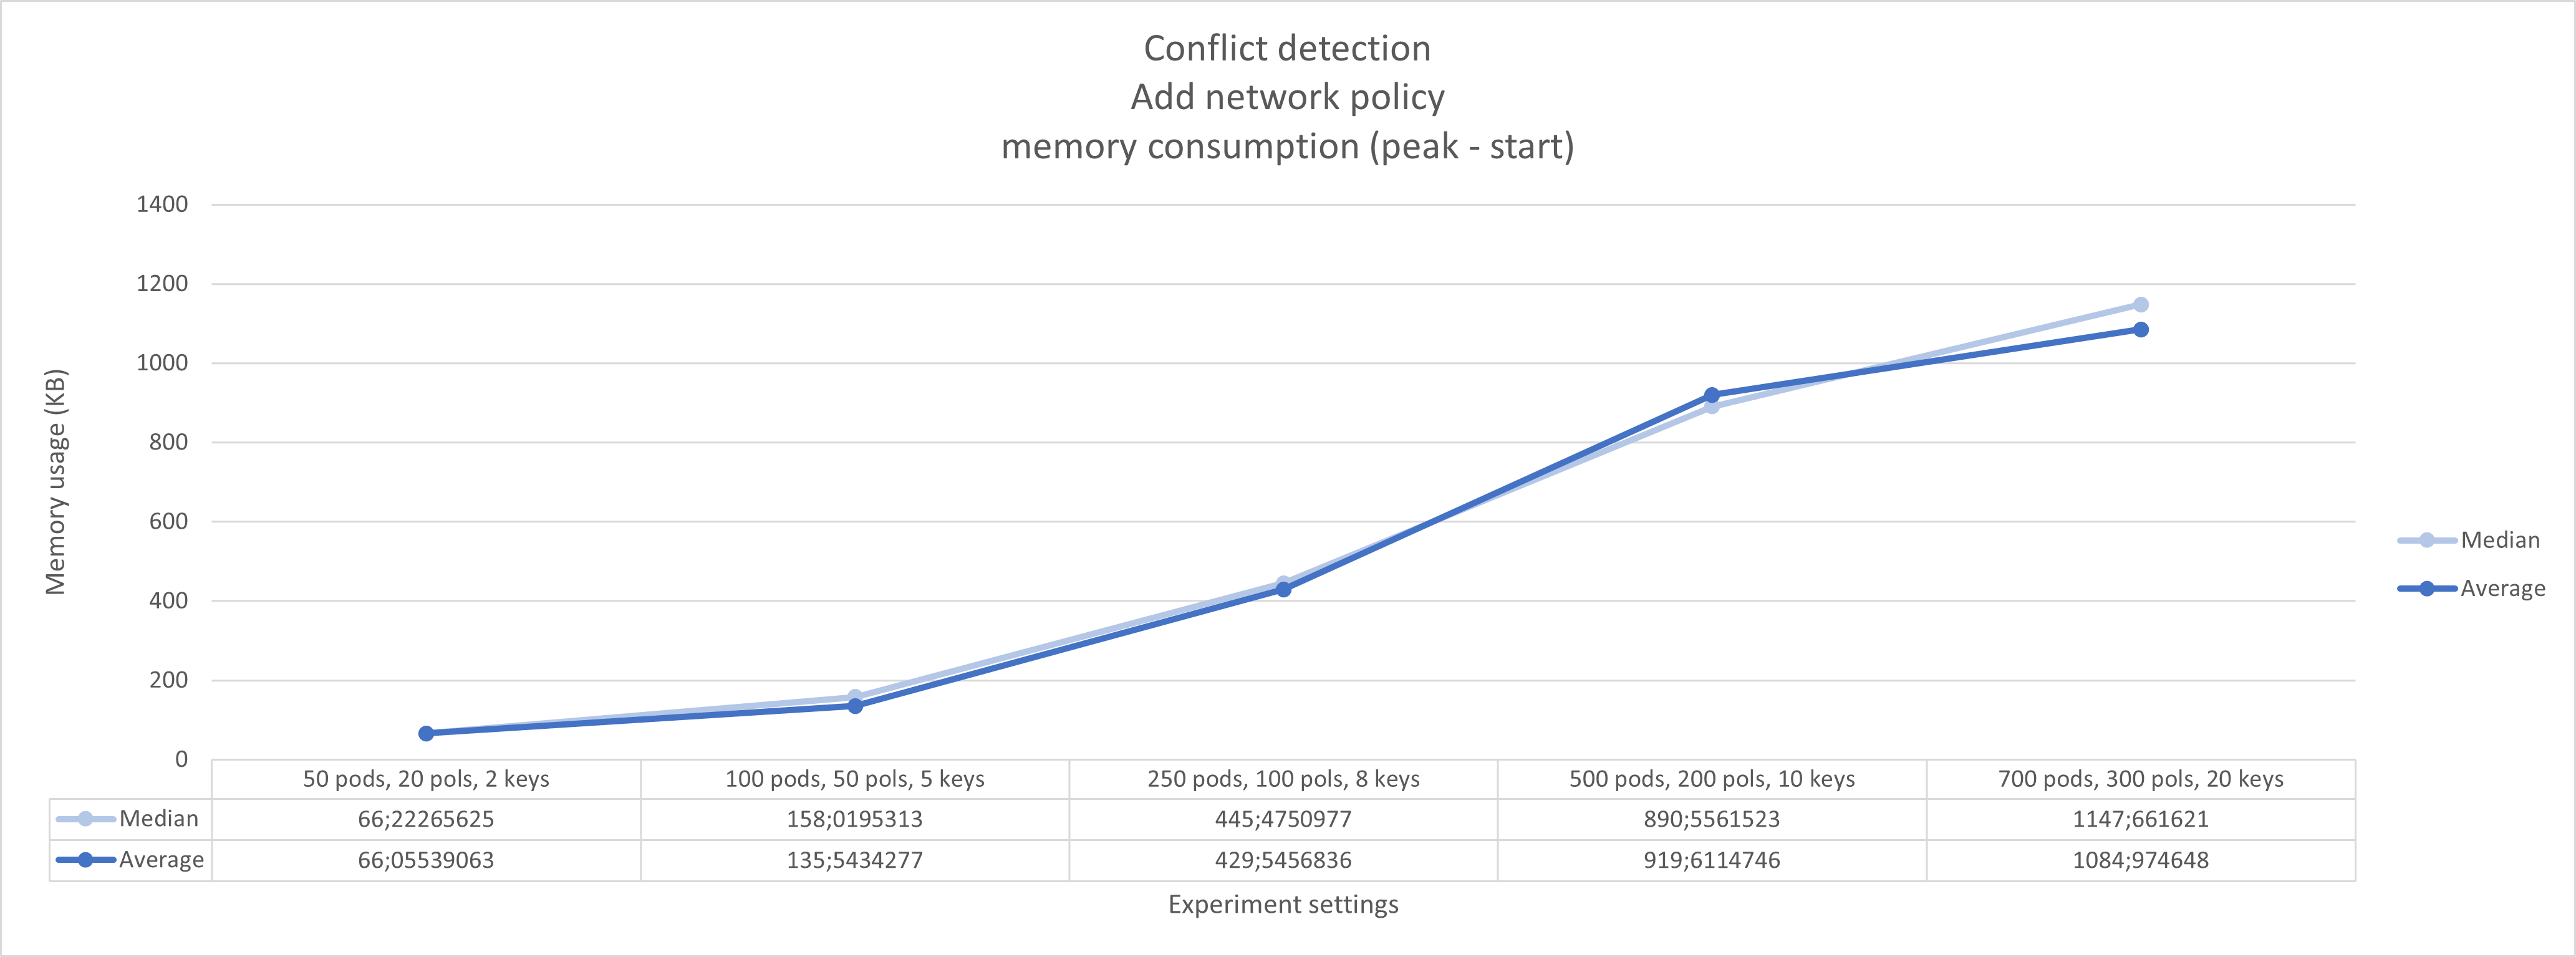
\includegraphics[width=\textwidth]{images/experiment2/addNP-memory-conflict.png}
    \caption{conflict detection memory consumption - add network policy}
    \label{fig:exp2-addNP-memory-conflict}
\end{figure}
\begin{figure}[H]
    \centering
    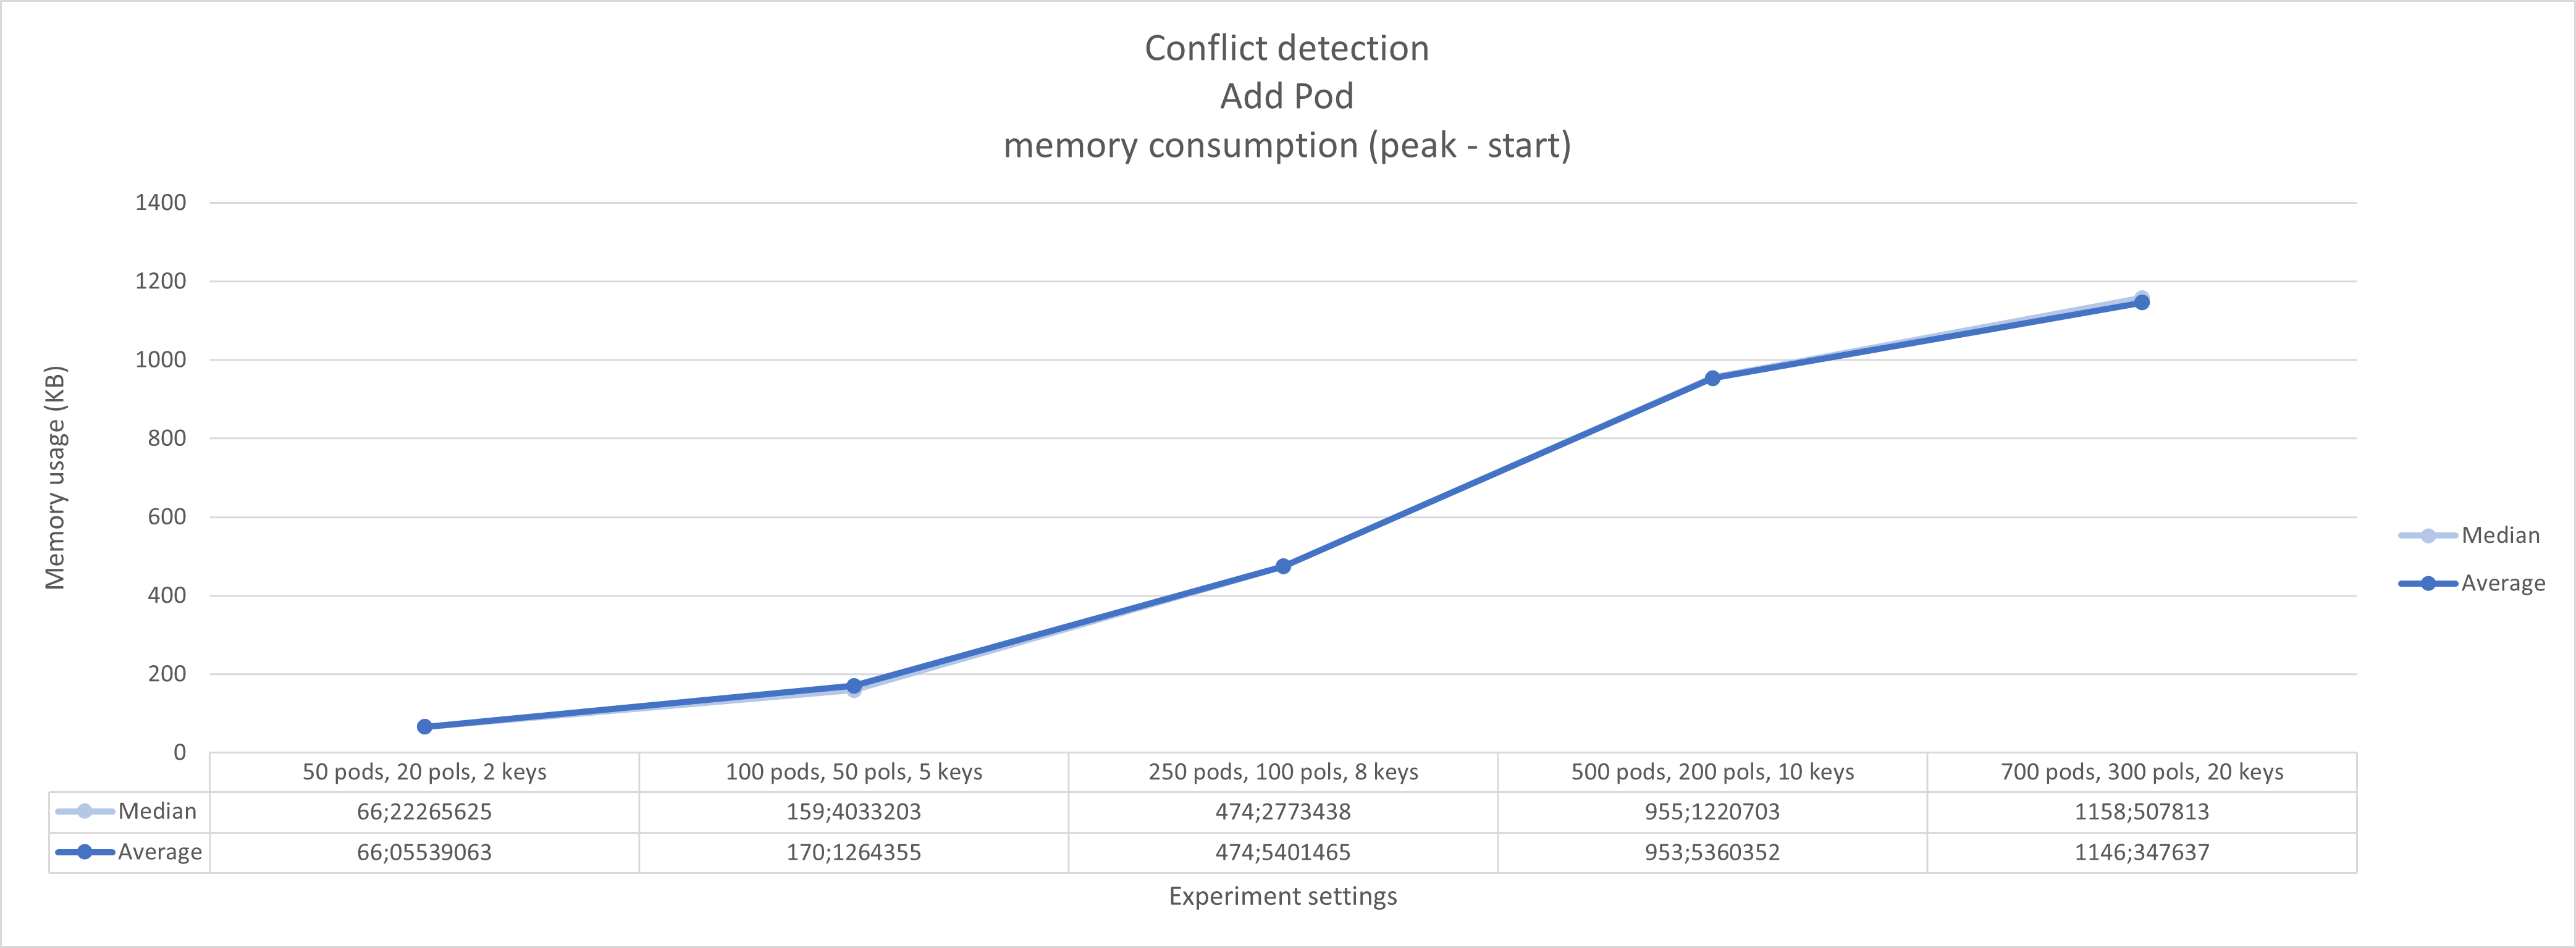
\includegraphics[width=\textwidth]{images/experiment2/addPod-memory-conflict.png}
    \caption{conflict detection memory consumption - add container}
    \label{fig:exp2-addPod-memory-conflict}
\end{figure}
\begin{figure}[H]
    \centering
    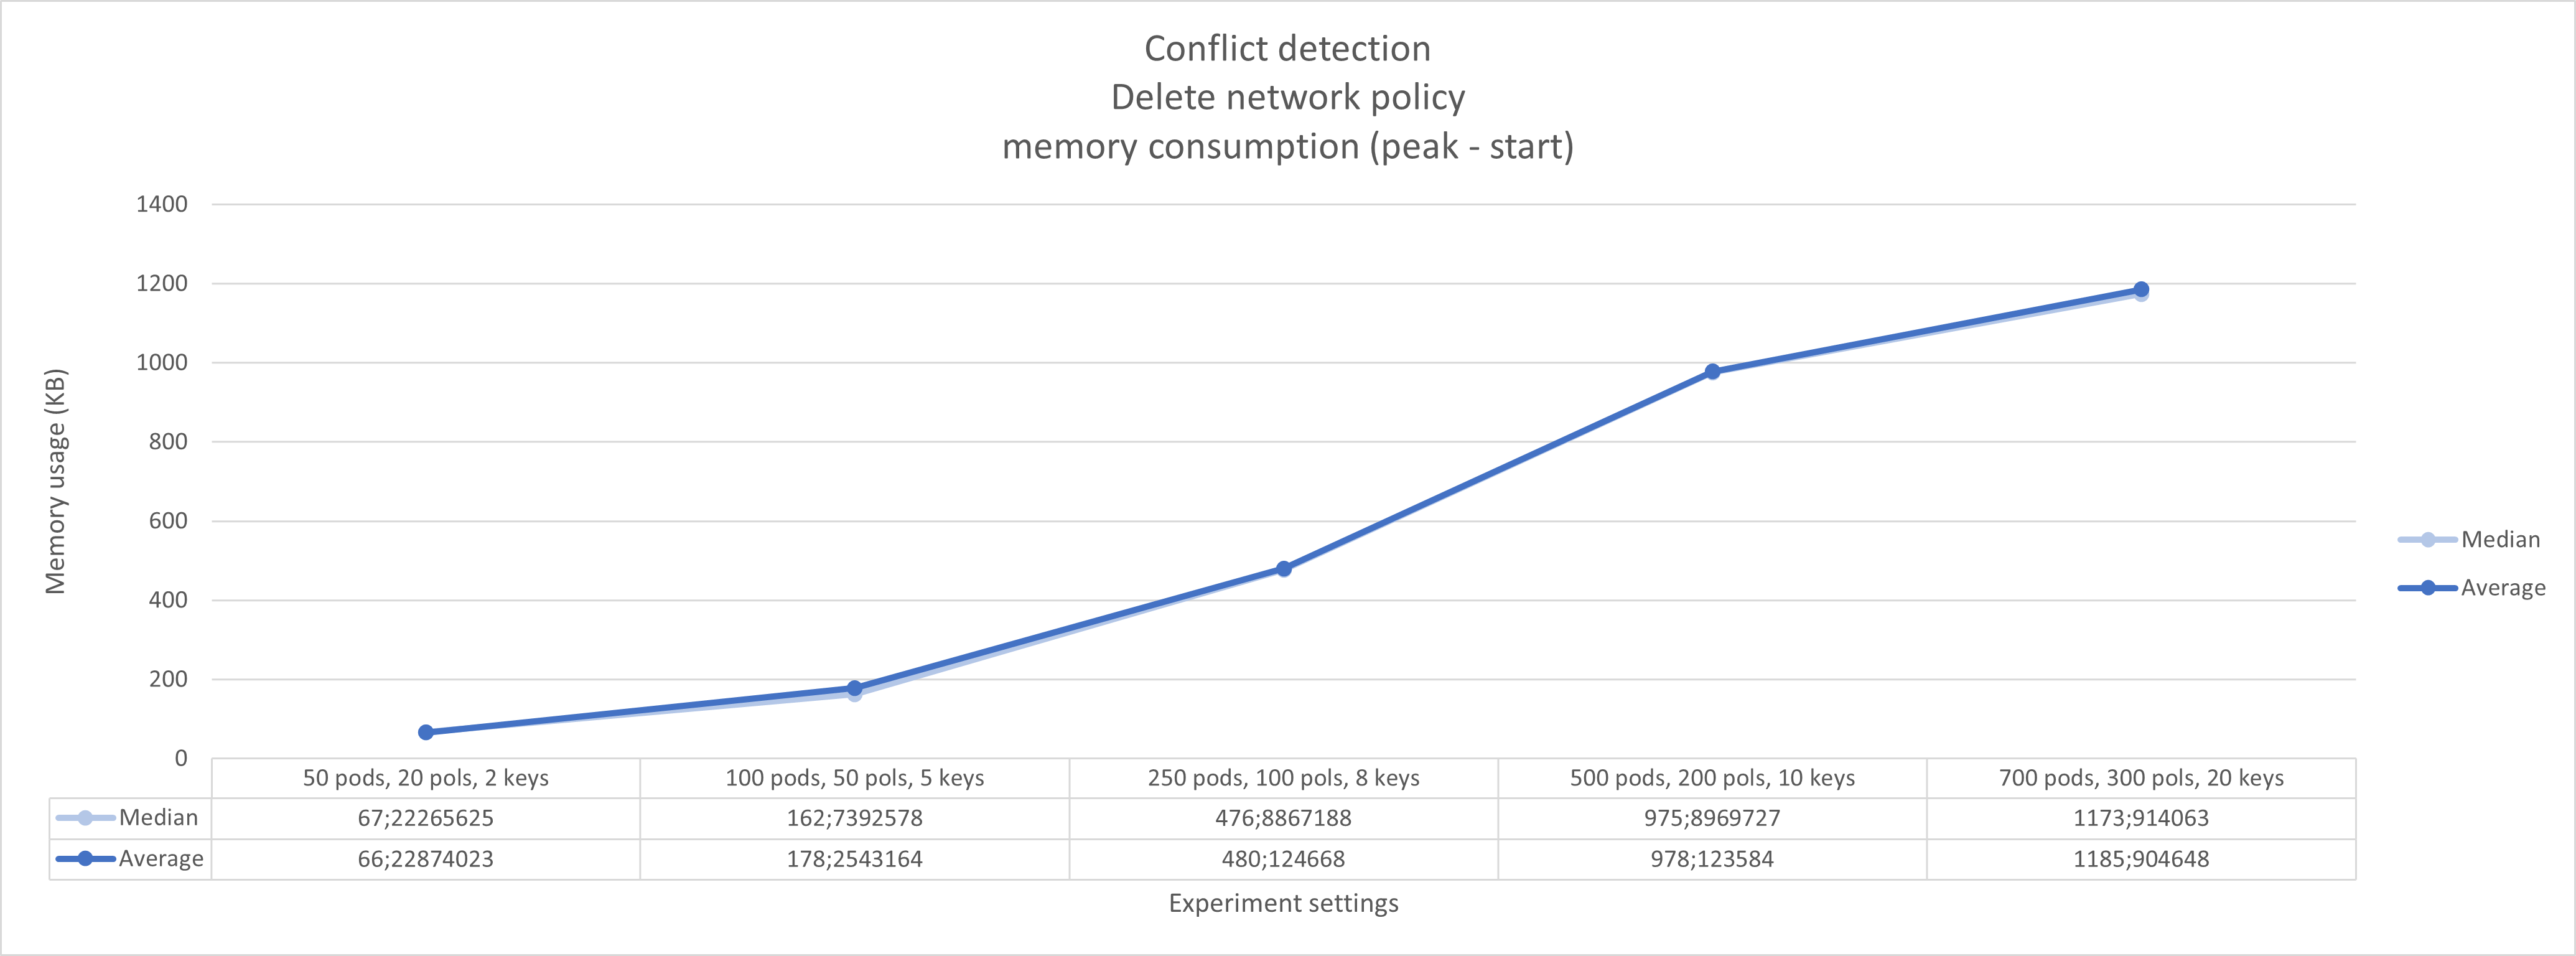
\includegraphics[width=\textwidth]{images/experiment2/delNP-memory-conflict.png}
    \caption{conflict detection memory consumption - delete network policy}
    \label{fig:exp2-delNP-memory-conflict}
\end{figure}
\begin{figure}[H]
    \centering
    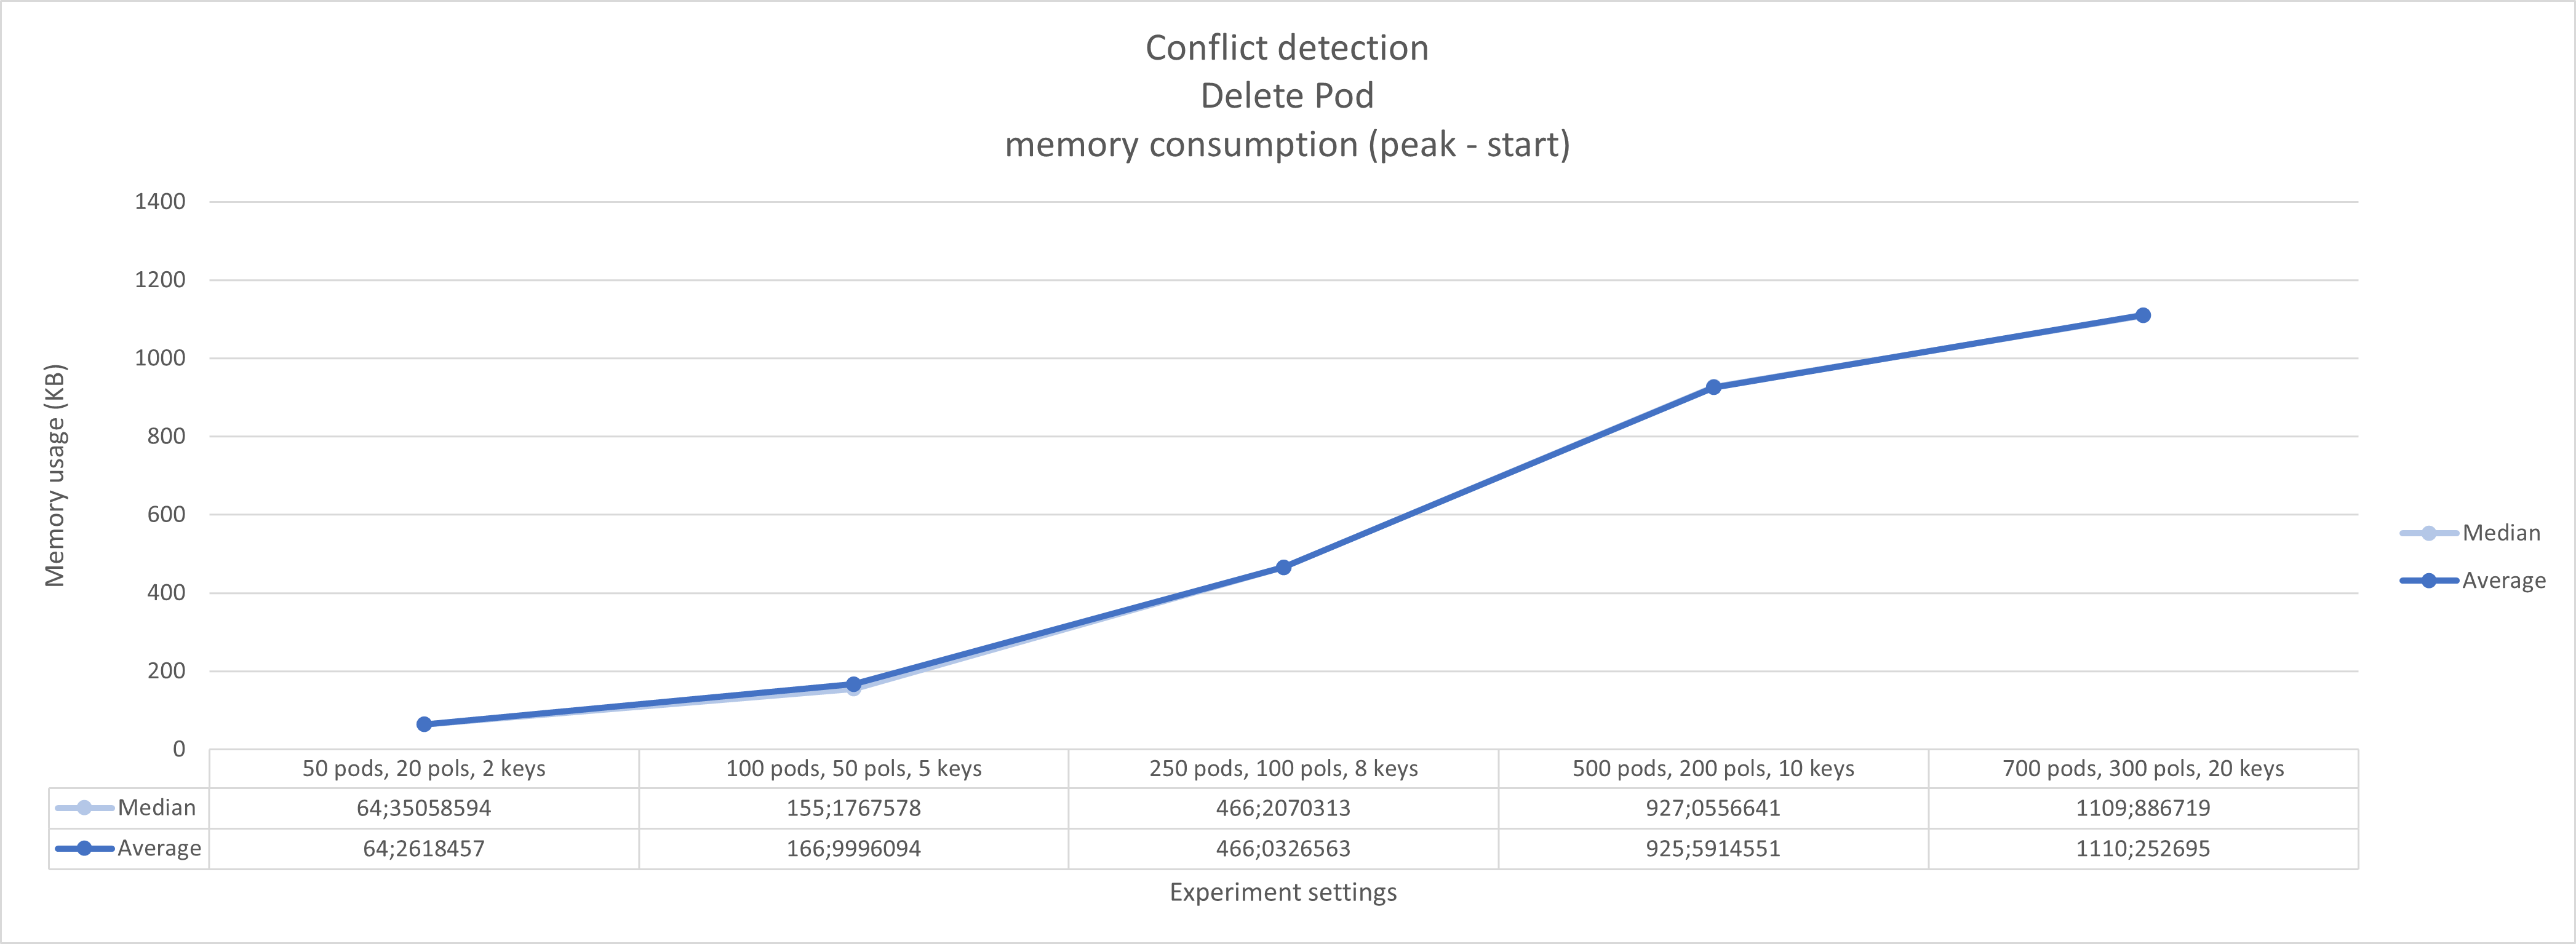
\includegraphics[width=\textwidth]{images/experiment2/delPod-memory-conflict.png}
    \caption{conflict detection memory consumption - delete container}
    \label{fig:exp2-delPod-memory-conflict}
\end{figure}


% =========================================
\section{Evaluation conclusion} \label{sec:conclusion}
We now combine the most important conclusions from these evaluation experiments into an overview:
\begin{itemize}
	\item Our incremental approach for updating the cluster state becomes faster than Kano's generative approach when we pass a certain cluster size threshold. This threshold changes depending on the cluster setup and the number of matches between label selectors in network policies and labels in pods. 
	\item The biggest drawback of the incremental update approach is the higher memory consumption due to the storage of the last cluster state compared to the generative approach. We must note however that the generative approach should be adapted to be usable for conflict detection in the algorithm and would require some extra variables which could lead to more memory usage as well.
	\item Updating the reachability matrix is the biggest contributor to time consumption whereas the conflict detection itself only adds slight overhead.
	\item Both memory and time consumption grow as the number of containers and network policies in the cluster increases. The biggest contributor to time consumption is the number of connections between containers that are defined by network policies.
\end{itemize}

\cleardoublepage


\newpage
%!TeX root=../../main.tex
\chapter{Conclusion}                                 \label{ch:conclusion}

%======================================
\section{Overview} \label{sec:overview}
In this thesis we reseached the Kubernetes technology stack regarding network security and defined the possibility af conflicts rising within due to misconfigurations between different layers of the stack. After we defined our problem statement we researched existing state-of-the art solutions regarding these conflicts and identified a knowledge gap within the current solutions as well as a possibility for improvement for Kano, an existing research solution. We continued by leveraging Kano's ideas to implement our algorithm that detects and reports on these conflicts. The implementation uses a incremental approach of updating the last locally saved cluster state, triggered by the monitoring and capturing of events that influence the connections between containers. 
\\[10pt]

In our evaluation we compared the incremental update functionality of our implementation against Kano's generative approach and concluded that the generative approach is faster than our incrementel solution for smaller clusters, whereas our incremental approach outperforms Kano's when the cluster becomes sufficiently large. A drawback of our incremental approach is the increased memory usage due to the storage of cluster state information as well as extra data required for the conflict detection \todo{Also say this in evaluation chapter}. In our second experiment we evaluated the general time and memory consumption for our entire conflict detection algorithm \todo{finish this}
\\[10pt]

%======================================
\section{footnote} \label{sec:footnote}
\todo{Different section name}
%Kano paper 2
%gitlab reference?

%======================================
\section{Future work} \label{sec:futurework}
We briefly mentioned a startup-verification method to detect already existing conflicts within the cluster, which is implemented but remains untested due to time constraints for this thesis. When the memory consumption of the implemented algorithm proves to be too excessive the generative approach combined with the conflict detection could possibly be executed periodically to confirm the conflict-free state of the cluster.
\\[10pt]

The solution algorithm does not monitor cloud level changes to the cluster but instead mimicks it by generating randomised Openstack security groups and their rules. Future work could include the continuous monitoring for events that influence inter-VM connections similarly to the implemented cluster-layer watcher, upon the capturing of which conflict detection gets triggered as well.
\\[10pt]



\cleardoublepage




\newpage
\bibliographystyle{IEEEtran}
\bibliography{sources/sources}


\newpage
% ----------------------- Achterblad ------------------------------
% Vergeet niet de tekst aan te passen:
% - Afdeling
% - Adres van de afdeling
% - Telefoon en faxnummer
% -----------------------------------------------------------------
\thispagestyle{empty}
\sffamily
%
\begin{textblock}{191}(113,-11)
{\color{blueline}\rule{160pt}{5.5pt}}
\end{textblock}
%
\begin{textblock}{191}(168,-11)
{\color{blueline}\rule{5.5pt}{59pt}}
\end{textblock}
%
\begin{textblock}{183}(-24,-11)
\textblockcolour{}
\flushright
\fontsize{7}{7.5}\selectfont
\textbf{DEPARTMENT OF COMPUTER SCIENCE}\\
Celestijnenlaan 200 A box 2402\\
3000 LEUVEN, BELGI\"{E}\\
tel. + 32 16 32 77 00\\
fax + 32 16 32 79 96\\
wms.cs.kuleuven.be/cs/\\
\end{textblock}
%
\begin{textblock}{191}(154,-7)
\textblockcolour{}
\includegraphics*[height=16.5truemm]{backpage/sedes}
\end{textblock}
%
\begin{textblock}{191}(-20,235)
{\color{bluetitle}\rule{544pt}{55pt}}
\end{textblock}
\end{document}
